
%% Based on a TeXnicCenter-Template, which was
%% created by Christoph Börensen
%% and slightly modified by Tino Weinkauf.
%%%%%%%%%%%%%%%%%%%%%%%%%%%%%%%%%%%%%%%%%%%%%%%%%%%%%%%%%%%%%

\documentclass[a4paper,12pt]{article} %scrartcl This is a special class provided by the KOMA script, which does a lot of adjustments to adapt the standard LaTeX classes to european habits, change to [a4paper,12pt,twoside] for doublesided layout


%########################### Preferences #################################


% ******** vmargin settings *********
\usepackage{vmargin} %This give you full control over the used page arae, it maybe not the idea od Latex to do so, but I wanted to reduce to amount of white space on the page
\setpapersize{A4}
\setmargins{3.5cm}%			%linker Rand, left edge
		   {1.5cm}%     %oberer Rand, top edge
           {14.7cm}%		%Textbreite, text width
           {23.42cm}%   %Texthoehe, text hight
           {30pt}%			%Kopfzeilenhöhe, header hight
           {1cm}%   	  %Kopfzeilenabstand, header distance
           {0pt}%				%Fußzeilenhoehe footer hight
           {2cm}%    	  %Fusszeilenabstand, footer distance   
\setlength{\parindent}{0pt}  % keine Einrückung nach Absatz

% ********* Font definiton ************
\usepackage{t1enc} % as usual
\usepackage[latin1]{inputenc} % as usual
\usepackage{times}		
\usepackage{fancyhdr} %%%% define chead, cfoot
\usepackage[table]{xcolor}
\usepackage{longtable}
\usepackage{booktabs}
\usepackage{tabularx}
\usepackage{wallpaper}

% ********* for code listing ************
\usepackage{listings}  
\usepackage{color}
\definecolor{gray}{rgb}{0.4,0.4,0.4}
\definecolor{darkblue}{rgb}{0.0,0.0,0.6}
\definecolor{cyan}{rgb}{0.0,0.6,0.6}

\lstloadlanguages{XML}

%\lstdefinelanguage{XML}
%{
  %morestring=[b]",
  %morestring=[s]{>}{<},
%%  morecomment=[s]{<?}{?>},
  %morecomment=[s][\color{orange}]{<!--}{-->},
  %stringstyle=\color{black},
  %identifierstyle=\color{darkblue},
  %keywordstyle=\color{red},
  %morekeywords={xmlns,version,type,num},
	%showstringspaces=false,
%}


%\usepackage{mathptmx}  	%mathematical fonts for use with times, I encountered some problems using this package togather with pdftex, which I was not able to resolve

% ********* Graphics definition *******
%\usepackage[pdftex]{graphicx} % required to import graphic files
\usepackage{eso-pic} % these two are required to add the little picture on top of every page
\usepackage{everyshi} % these two are required to add the little picture on top of every page
\renewcommand{\floatpagefraction}{0.7} %default:0.5 allows two big pictures on one page
\usepackage{wrapfig}

%********** Enybeling Hyperlinks *******
\usepackage[pdfborder=000,pdftex=true]{hyperref}% this enables jumping from a reference and table of content in the pdf file to its target

% ********* Table layout **************
\usepackage{booktabs}	  	%design of table, has an excellent documentation
\usepackage{multirow}     % multirows in tables

% ********* Caption Layout ************
\usepackage{ccaption} % allows special formating of the captions
\captionnamefont{\bf\footnotesize\sffamily} % defines the font of the caption name (e.g. Figure: or Table:)
\captiontitlefont{\footnotesize\sffamily} % defines the font of the caption text (same as above, but not bold)
\setlength{\abovecaptionskip}{0mm} %lowers the distace of captions to the figure

%\usepackage{scrpage2} %header and footer using the options for the KOMA script % defines cfoot chead; cannot be used at the same time as fancyhdr
\newcommand{\headfont}{\footnotesize\sffamily} % font for the header
\newcommand{\pnumfont}{\footnotesize\sffamily} % font for the pagenumbers

\usepackage{helvet}
\renewcommand{\familydefault}{\sfdefault}

% set colors for links and URLs
\usepackage{hyperref}
\hypersetup{
	colorlinks=true,
	linkcolor=black,
	urlcolor=blue}


%this defines the page style for the first pages: all empty
%\renewpagestyle{plain}%
%	{(\textwidth,0pt)%
%		{\hfill}{\hfill}{\hfill}%
%	(\textwidth,0pt)}%
%	{(\textwidth,0pt)%	
%		{\hfill}{\hfill}{\hfill}%
%	(\textwidth,0pt)}

% CUSTOM LISTING FORMAT

\lstdefinestyle{lststyle}{
%	belowcaptionskip=1\baselineskip,
	breaklines=true,
%	frame=L,
	xleftmargin=\parindent,
%	language=C,
	showstringspaces=false,
	basicstyle=\footnotesize\ttfamily,
%	keywordstyle=\bfseries\color{green!40!black},
%	commentstyle=\itshape\color{purple!40!black},
%	identifierstyle=\color{blue},
	stringstyle=\color{orange},
}
\lstset{escapechar=@,style=lststyle}
% JSON format
\usepackage{listings}
\usepackage{xcolor}

\colorlet{punct}{red!60!black}
\definecolor{background}{HTML}{EEEEEE}
\definecolor{delim}{RGB}{20,105,176}
\colorlet{numb}{magenta!60!black}

\lstdefinelanguage{json}{
	basicstyle=\small\ttfamily,
	numbers=left,
	numberstyle=\scriptsize,
	stepnumber=1,
	numbersep=8pt,
	showstringspaces=false,
	breaklines=true,
	frame=lines,
	backgroundcolor=\color{background},
	literate=
	*{0}{{{\color{numb}0}}}{1}
	{1}{{{\color{numb}1}}}{1}
	{2}{{{\color{numb}2}}}{1}
	{3}{{{\color{numb}3}}}{1}
	{4}{{{\color{numb}4}}}{1}
	{5}{{{\color{numb}5}}}{1}
	{6}{{{\color{numb}6}}}{1}
	{7}{{{\color{numb}7}}}{1}
	{8}{{{\color{numb}8}}}{1}
	{9}{{{\color{numb}9}}}{1}
	{:}{{{\color{punct}{:}}}}{1}
	{,}{{{\color{punct}{,}}}}{1}
	{\{}{{{\color{delim}{\{}}}}{1}
	{\}}{{{\color{delim}{\}}}}}{1}
	{[}{{{\color{delim}{[}}}}{1}
	{]}{{{\color{delim}{]}}}}{1},
}

%----------------------------------------------------------------------------------------
%	BEGIN DOCUMENT
%----------------------------------------------------------------------------------------

\pagestyle{plain} % on headers or footers on the first page


%%%%%%%%%%%%%%%%%%%%%%%%%%%%%%%%%%%%%%%%%%%%%%%%%%%%%%%%%%%%%%%%%%%
 %%%%%%%%%%%%%         CHANGE VERSION NUMBER HERE    %%%%%%%%%%%
\newcommand{\version}{2.10.5}
 %%%%%%%%%%%%%%%%%%%%%%%%%%%%%%%%%%%%%%%%%%%%%%%%%%%%%%%%%%%%%%%
 %%%%%%%%%%%%%%%%%%%%%%%%%%%%%%%%%%%%%%%%%%%%%%%%%%%%%%%%%%%%%%%%%%%
 
\begin{document}

%----------------------------------------------------------------------------------------
%	TITLE PAGE
%----------------------------------------------------------------------------------------
\begin{titlepage}
	\centering
	{\scshape\Huge \textbf{ PRo3D \version} \par}
	{\scshape\Large User Manual\par}
	\vspace{1.cm}
	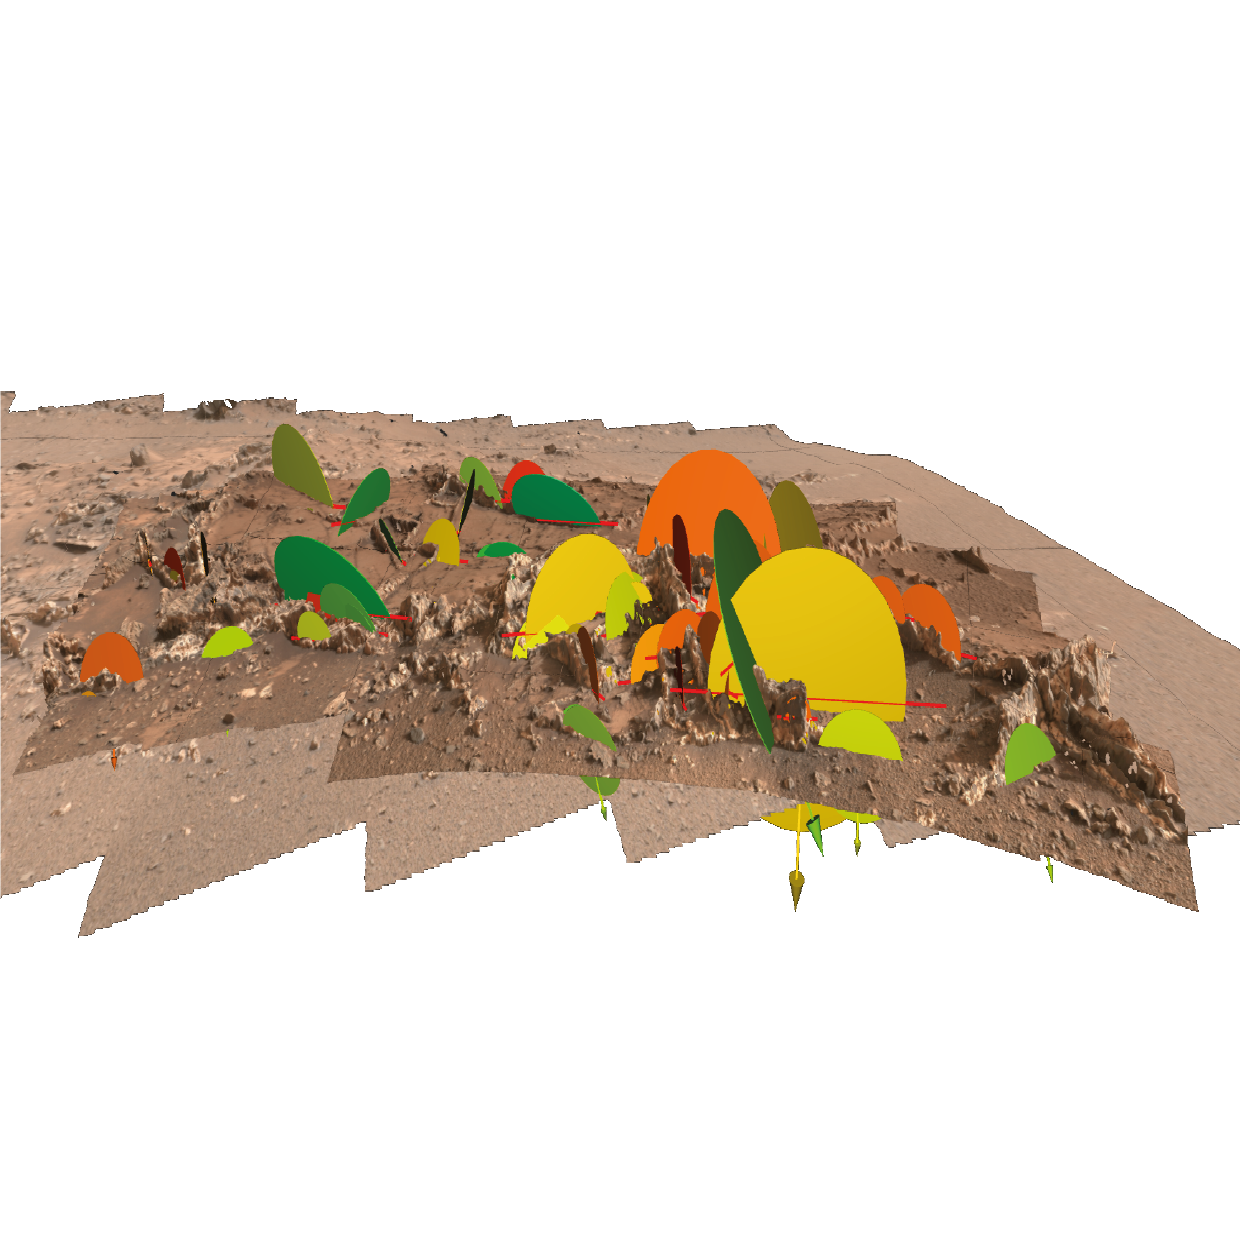
\includegraphics[width=1.0\textwidth]{pics/CoverPic.png}\par\vspace{1cm}		
	{\large Authors: \par
	Thomas Ortner, Laura Fritz, Rebecca Nowak}
	\vfill
	% Bottom of the page
	{Last Updated: \today\par}
\end{titlepage}

\newpage

\pagestyle{fancy} % now we want to have headers and footers

%----------------------------------------------------------------------------------------
%	Header and Footer
%----------------------------------------------------------------------------------------
\fancyhf{} %alle Kopf- und Fußzeilenfelder bereinigen
\fancyhead[R]{} %Kopfzeile rechts
\fancyhead[C]{} %zentrierte Kopfzeile
\fancyhead[L]{
\includegraphics[height=30pt]{pics/logosSUM.png}} %Kopfzeile links
\renewcommand{\headrulewidth}{0.4pt} %obere Trennlinie

\fancyfoot[L]{{PRo3D \version}}

\fancyfoot[R]{\thepage} 
\renewcommand{\footrulewidth}{0.4pt} %untere Trennlinie

%----------------------------------------------------------------------------------------
%	Change Records 
%----------------------------------------------------------------------------------------

%\begin{table}[h]
	%\centering
	%
		%\caption{\textbf{Change Records}}
		%\label{tab:changeRecs}
		%
		%\rowcolors{1}{lightgray}{white}
%
		%\begin{tabular}{c c p{7cm} p{3cm}}
			%\textbf{ISSUE} & \textbf{DATE} & \textbf{§ CHANGE RECORDS} & \textbf{AUTHOR} \\
			%\hline
			%1.0 & 2018-01-23 & Initial Version & Ortner, Fritz
		%\end{tabular}
%
%\end{table}

\newpage

%----------------------------------------------------------------------------------------
%	Table of Contents + List of Figures
%----------------------------------------------------------------------------------------
\tableofcontents
%\listoffigures

\newpage
%----------------------------------------------------------------------------------------
%	Section: Introduction
%----------------------------------------------------------------------------------------
%----------------------------------------------------------------------------------------
%	Section: Introduction
%----------------------------------------------------------------------------------------
\section{Introduction}

\begin{figure}[h]
    	\centering
    		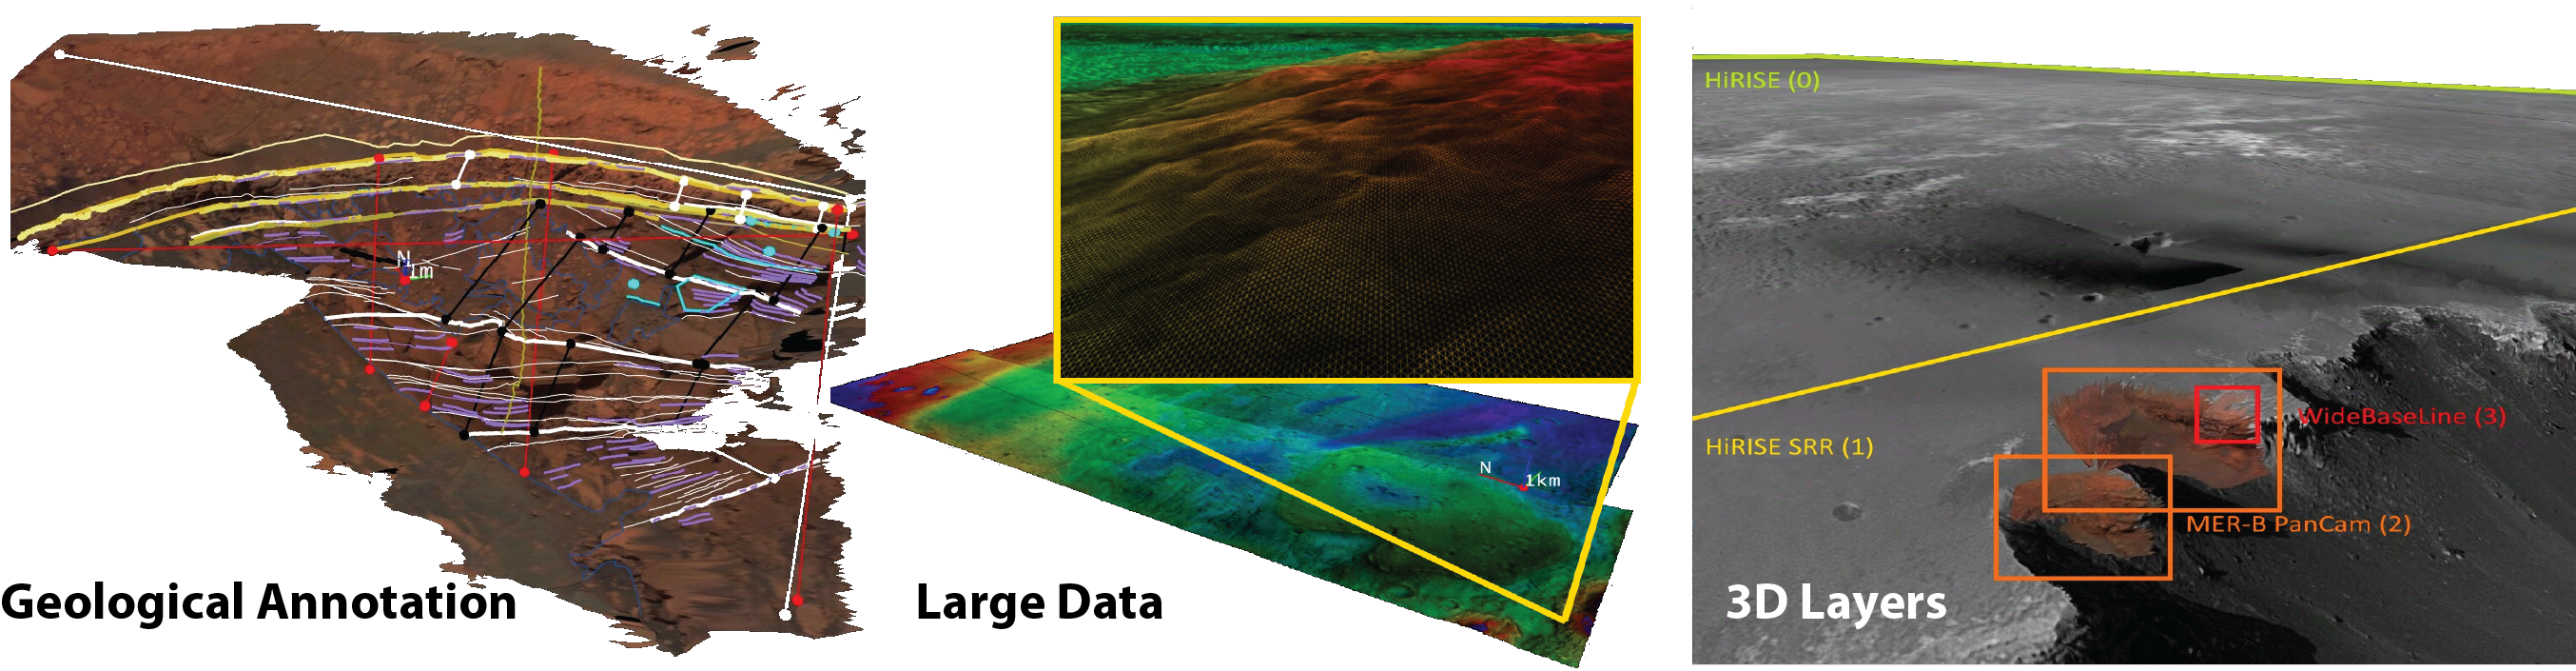
\includegraphics[width=1\textwidth]{pics/Features.png}
    	%\caption[Viewer Features]{}
    	\label{fig:Features}
   \end{figure}
	
PRo3D, short for \textbf{P}lanetary \textbf{Ro}botics \textbf{3D} Viewer, is an interactive 3D visualization tool to allow planetary scientists to work with high-resolution 3D reconstructions of the Martian surface.
%----------------------------------------------------------------------------------------
%	SubSection: Who uses PRo3D
%----------------------------------------------------------------------------------------
\subsection{Who uses PRo3D}
\label{sec:whoUsesP3D}

PRo3D aims to support planetary scientists in the course of NASA's and ESA's missions to find signs of life on the red planet by exploring high-resolution 3D surface reconstructions from orbiter and rover cameras.

For the past 5 years the development of PRo3D has been geared towards providing planetary \textbf{geologists} with interactive tools to digitize geological features on digital outcrop models (DOMs) on the Martian surface. During our fruitful cooperation with geologists from the Imperial College of London, PRo3D has emerged as their main tool to conduct remote geological analysis which lead to many publications and talks at various geological science venues.

Planetary geology is the most elaborately supported use-case of PRo3D, however we strive to expand our user groups to other use-cases, so we have also developed features for supporting science goals in \textbf{landing site selection} and \textbf{mission planning}.

%----------------------------------------------------------------------------------------
%	SubSection: Features
%----------------------------------------------------------------------------------------
\subsection{Features}
\label{sec:features}

\begin{itemize}
	\item \textbf{Geological Annotation}: PRo3D lets users pick points on the 3D surface at the full resolution of the data present. Our tools contain point, line, and polyline annotations, while line segments are projected onto the surface. Various measurements are computed at the highest possible accuracy, such as the distance along a 3D surface (waylength) or dip-and-strike orientations of sediment structures. 
	\item \textbf{Large Data}: Surface reconstructions from high-resolution satellite images can easily yield gigabytes of data in terms of geometry, imagery, and additional layers. With PRo3D users can explore huge datasets interactively and even perform measurements of topographic features. The displayed dataset on the right consists of 2GB of raw 3D position vectors, a 1GB elevation map, and 10GB of image data rendered at interactive framerates with commodity hardware, utilizing adjustable level-of-detail and out-of-core techniques. 
	\item \textbf{3D Layers}: Although, PRo3D is not a GIS system, we need to provide our users with typical GIS features to solve their geospatial problems, such as evaluating topographic or geological features. Our 3D layering technique allows a seamless integration of different reconstructions present at a single location. Unlike image or DTM layering we allow users to blend full 3D data by assigning rendering priorities, which is crucial to explore reconstructions from multiple rover camera instruments. 
	\item \textbf{Batch rendering of images:} PRo3D sports a command line interface that can be used to quickly render a large number of images without the hassle of using a graphical user interface.
\end{itemize}
%----------------------------------------------------------------------------------------
%	SubSection: Data
%----------------------------------------------------------------------------------------
\subsection{Data}
\label{sec:data}

Currently, PRo3D only supports reconstructions in the proprietary data format OPC (Ordered Point Clouds), basically consisting of hierarchically organized surface patches. These reconstructions stem from orbiter images and rover images and are produced by Joanneum Research by using the PRoViP processing pipeline. Many surface reconstructions have been generated from, for instance: HiRISE, MER-A, MER-B and MSL missions from various instruments. An ongoing project evaluates terrestrial applicability of PRo3D and the PRoViP pipeline by capturing outcrops in the UK. 


%----------------------------------------------------------------------------------------
%	Section: Start
%----------------------------------------------------------------------------------------
%----------------------------------------------------------------------------------------
%	Section: Start
%----------------------------------------------------------------------------------------
\section{Start}
\label{sec:startViewer}

Start the viewer by clicking the PRo3D.exe and open the Menu in the top left of the window, shown in Figure~\ref{fig:StartMenu}.
\begin{figure}[h]
    	\centering
    		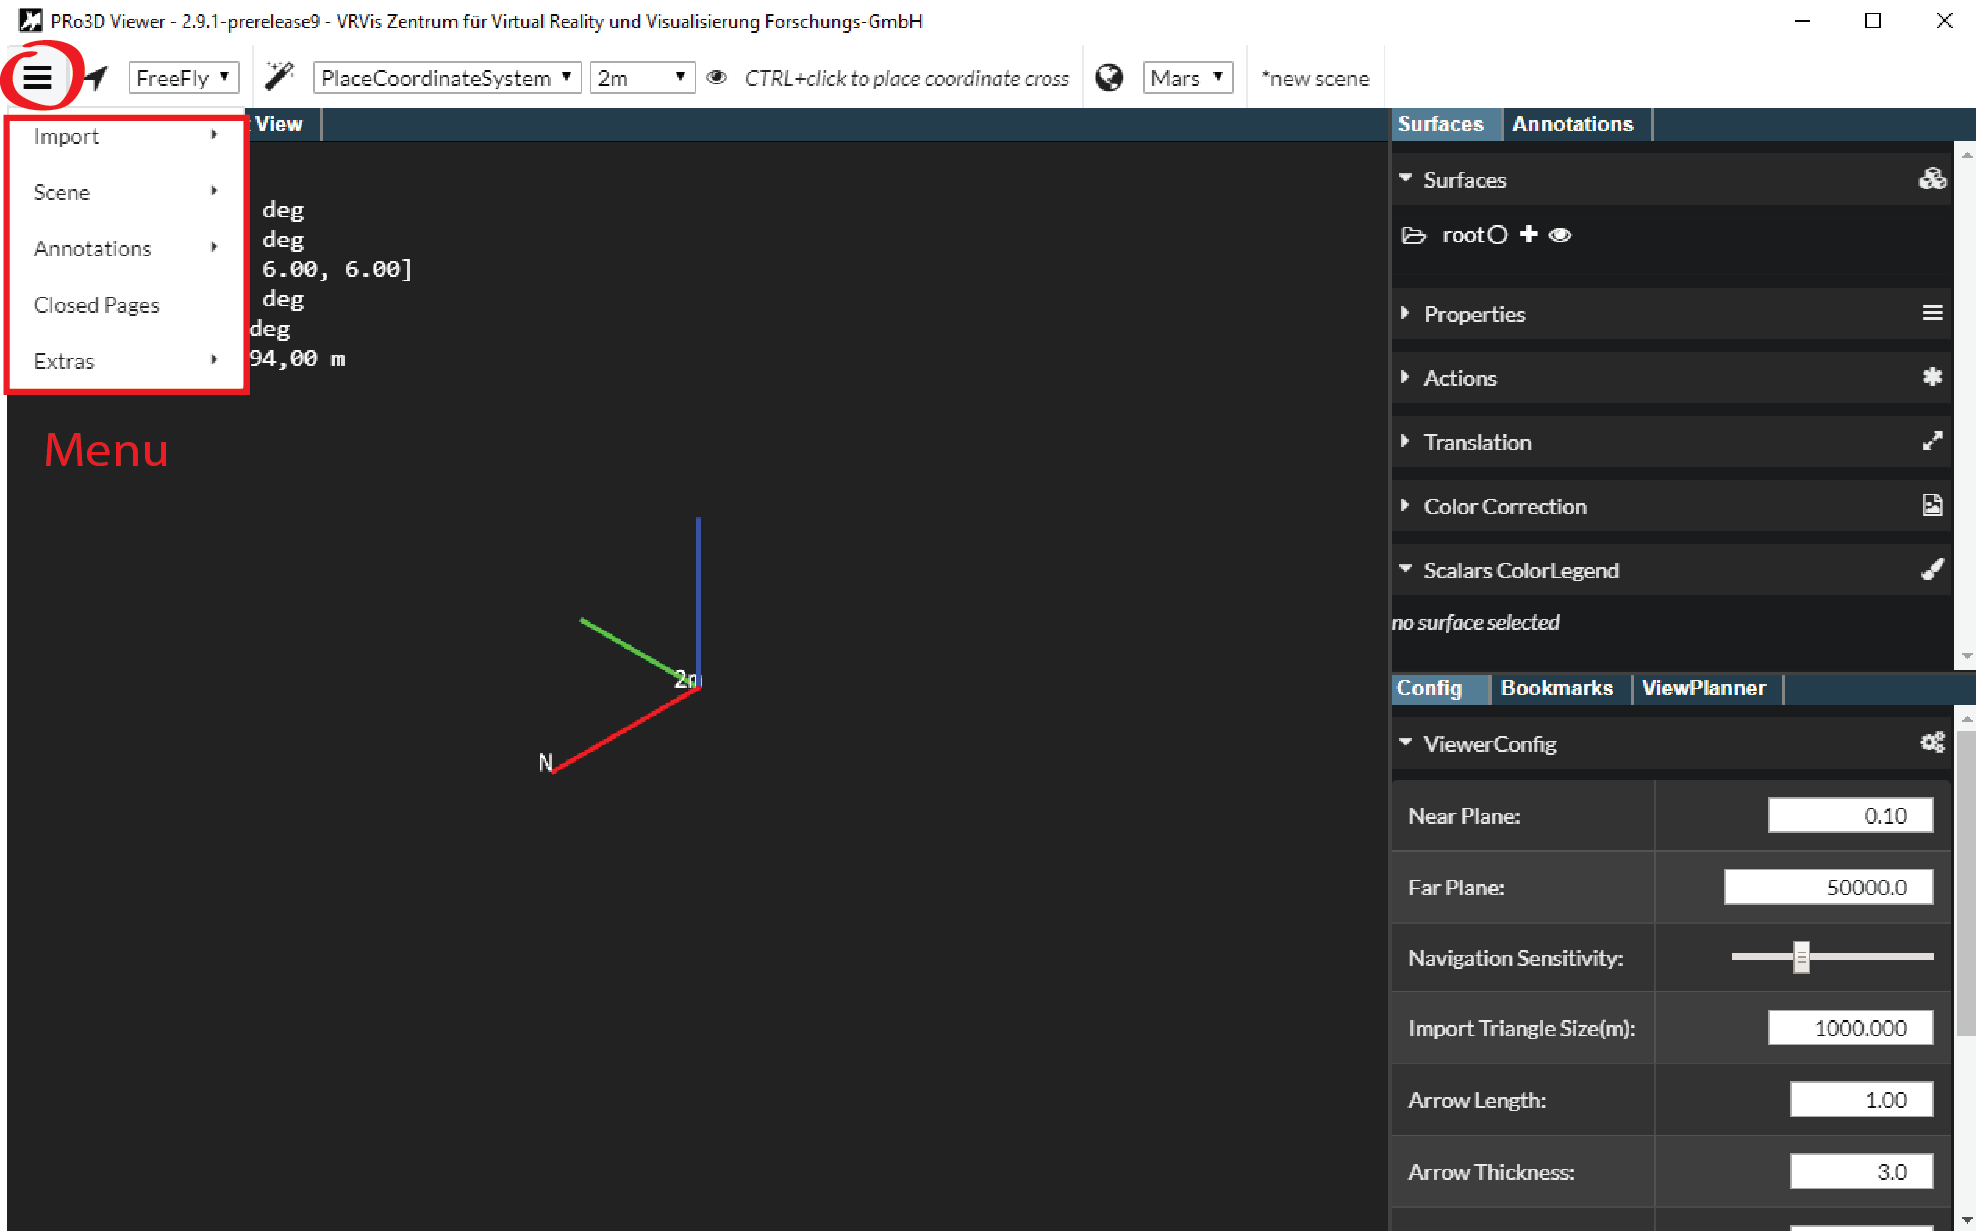
\includegraphics[width=1\textwidth]{pics/startAI.png}
    	\caption[Start Menu]{PRo3D Main Menu. }
    	\label{fig:StartMenu}
   \end{figure}

You have two options to start:
\begin{itemize}
	\item Add one or more surfaces and create a new scene, as described in the next Section~\ref{sec:addSurface}.
	\item Load an existing scene described in the Section~\ref{sec:loadScene}. 
\end{itemize}


%In the scene menu you have the following sections:
%\begin{itemize}
	%\item \textbf{Scene:}
	%\item \textbf{Recent:}
	%\item \textbf{Add Surface:}
	%\item \textbf{ImportAnnotationGroups:}
%\end{itemize}

%----------------------------------------------------------------------------------------
%	SubSection: Add Surface
%----------------------------------------------------------------------------------------
\subsection{Add Surface}
\label{sec:addSurface}

To add a new surface move the mouse to the ``Import'' tab in the menu (Figure~\ref{fig:StartMenu}). Click on the ``OPC'' tab to choose a surface (with ``OBJ'' you can import object files).
This opens the ``Select Folder'' window where you can choose one or more folders containing opc files as shown in Figure~\ref{fig:AddSurface}. Click the ``Select Folder'' button to confirm your selection. The surface is loaded into the viewer and listed in the ``Surface'' page in the right part of the window as shown in Figure~\ref{fig:NewSurface}, part A.
You can add more surfaces in the same way.
	
	\begin{figure}[h]
    	\centering
    		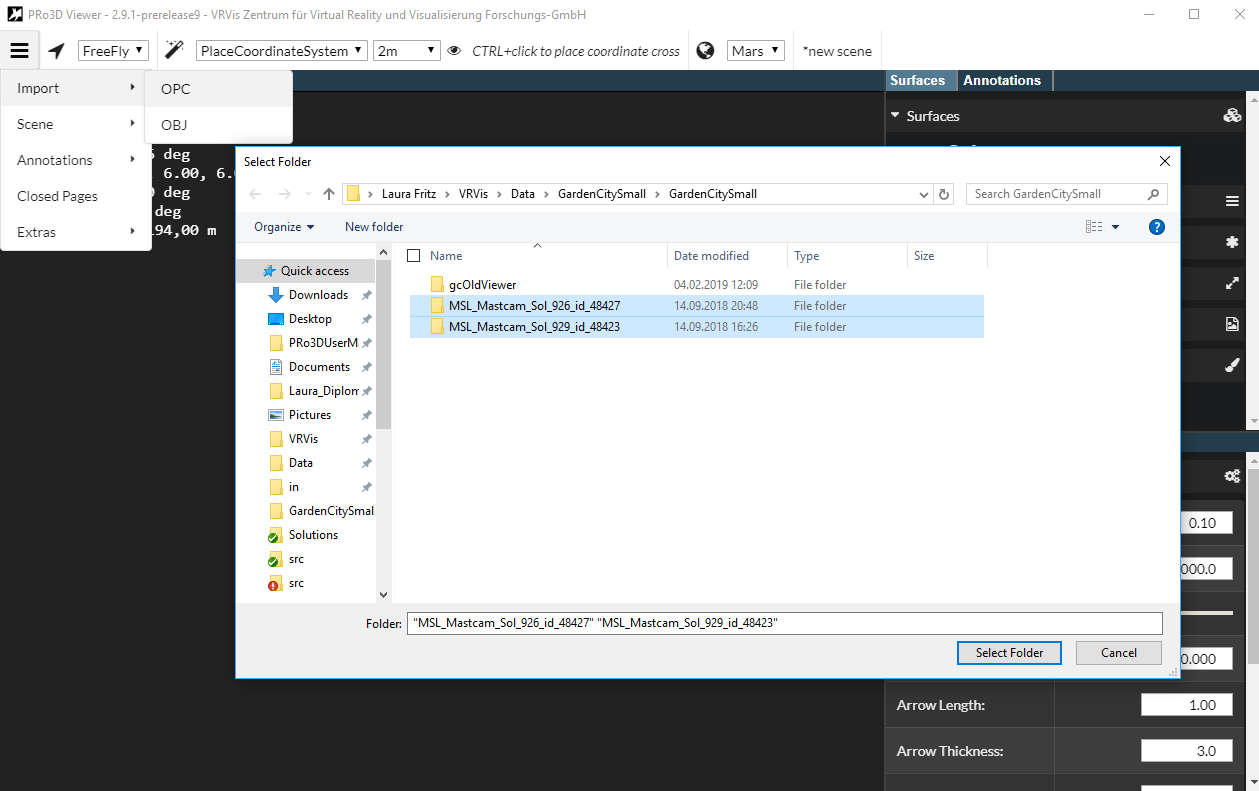
\includegraphics[width=1\textwidth]{pics/AddSurface.png}
    	\caption[Add Surface]{Add new surfaces to the scene.}
    	\label{fig:AddSurface}
   \end{figure}
	
	
Each surface has a little context menu below the surface's name in the list (Figure~\ref{fig:NewSurface}, B). Click the ``FlyTo'' button to see the surface in the main window. To see the surface's properties (Figure~\ref{fig:NewSurface}, C) click on the appropriate name in the list.
	
Finally, click ``Scene -> Save as...'' in the menu, name the scene and press the ``Save'' button (Figure~\ref{fig:saveScene}) to save the surfaces and your settings in a ``.scn'' file. The PRo3D viewer will load the scene automatically next time you start the viewer.
	
	\begin{figure}[h]
    	\centering
    		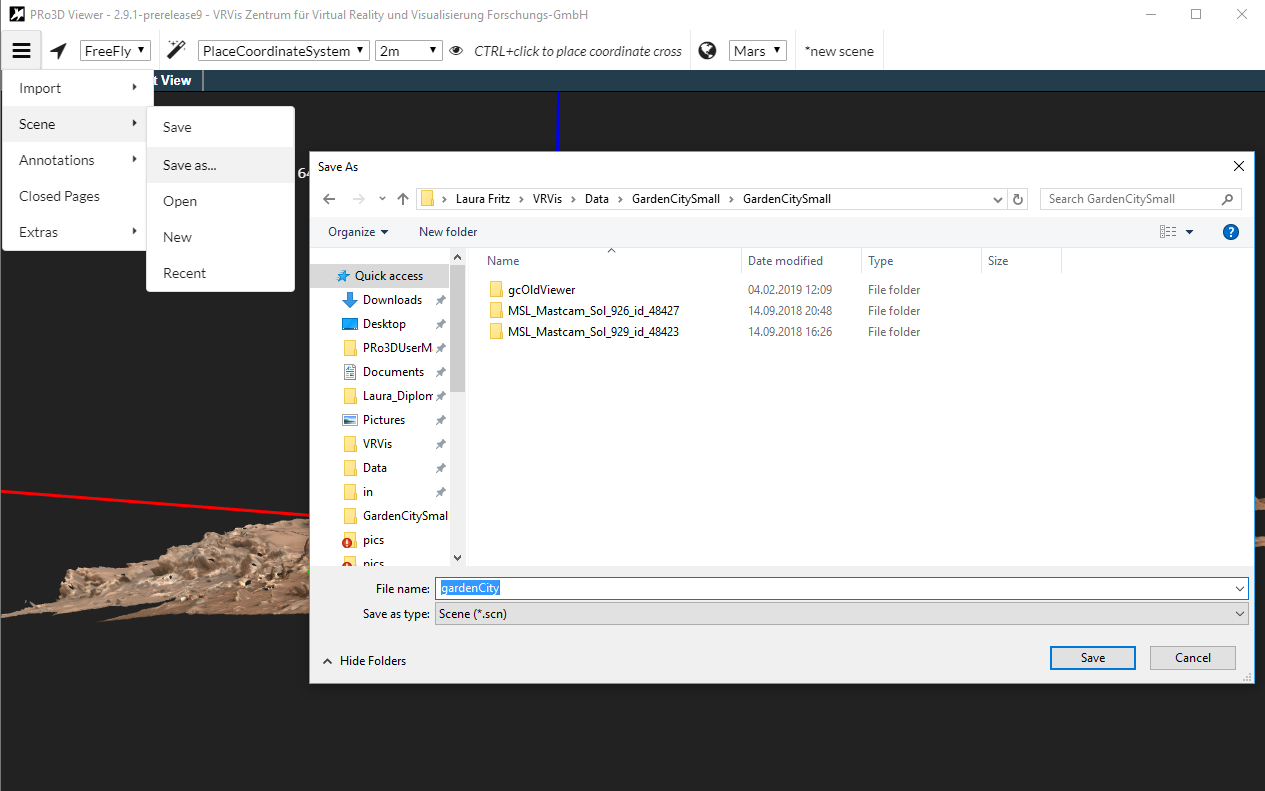
\includegraphics[width=1\textwidth]{pics/saveScene.png}
    	\caption[Save Scene]{Save the surfaces and settings as a scene. }
    	\label{fig:saveScene}
   \end{figure}
		
%----------------------------------------------------------------------------------------
%	SubSection: Load Scene
%----------------------------------------------------------------------------------------
\subsection{Load Scene}
\label{sec:loadScene}

Load an existing scene by selecting ``Scene -> Open'' in the \textbf{Scene} tab in the start menu (Figure~\ref{fig:StartMenu}).
Select the scene xml file in the directory of your choice and confirm your selection (Figure~\ref{fig:OpenScene}).
Then the scene is loaded (Figure~\ref{fig:NewSurface}). 

\begin{figure}[h]
    	\centering
    		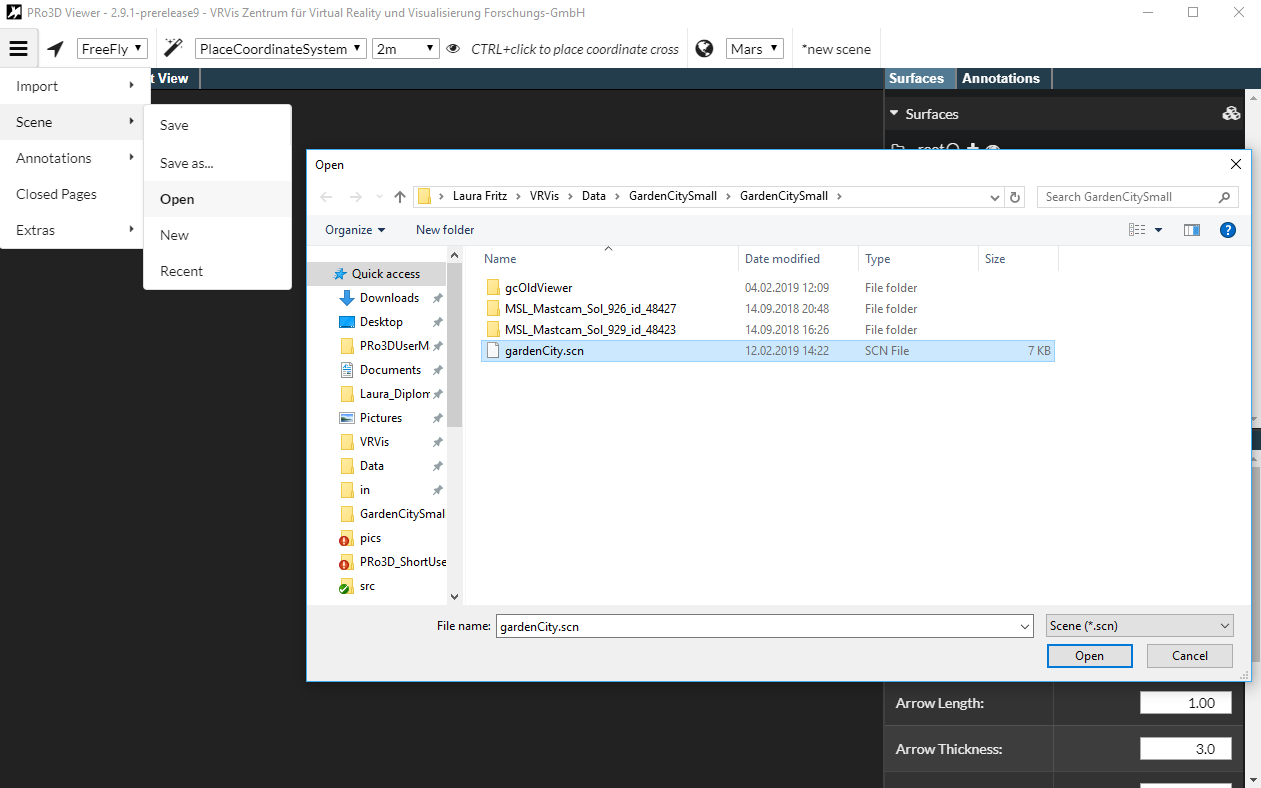
\includegraphics[width=1\textwidth]{pics/OpenScene.png}
    	\caption[Open Scene]{ Open a scene with either the ``Scene -> Open'' or the ``Scene -> Recent'' tab in the scene tab of the menu.}
    	\label{fig:OpenScene}
   \end{figure}
	
You can also load recent scene files with the ``Scenes -> Recent'' tab in the Scene tab of the menu . By hovering with the mouse over the tab,
a list of recent scenes opens. Click on the required scene name to load the scene.

\begin{figure}[h]
    	\centering
    		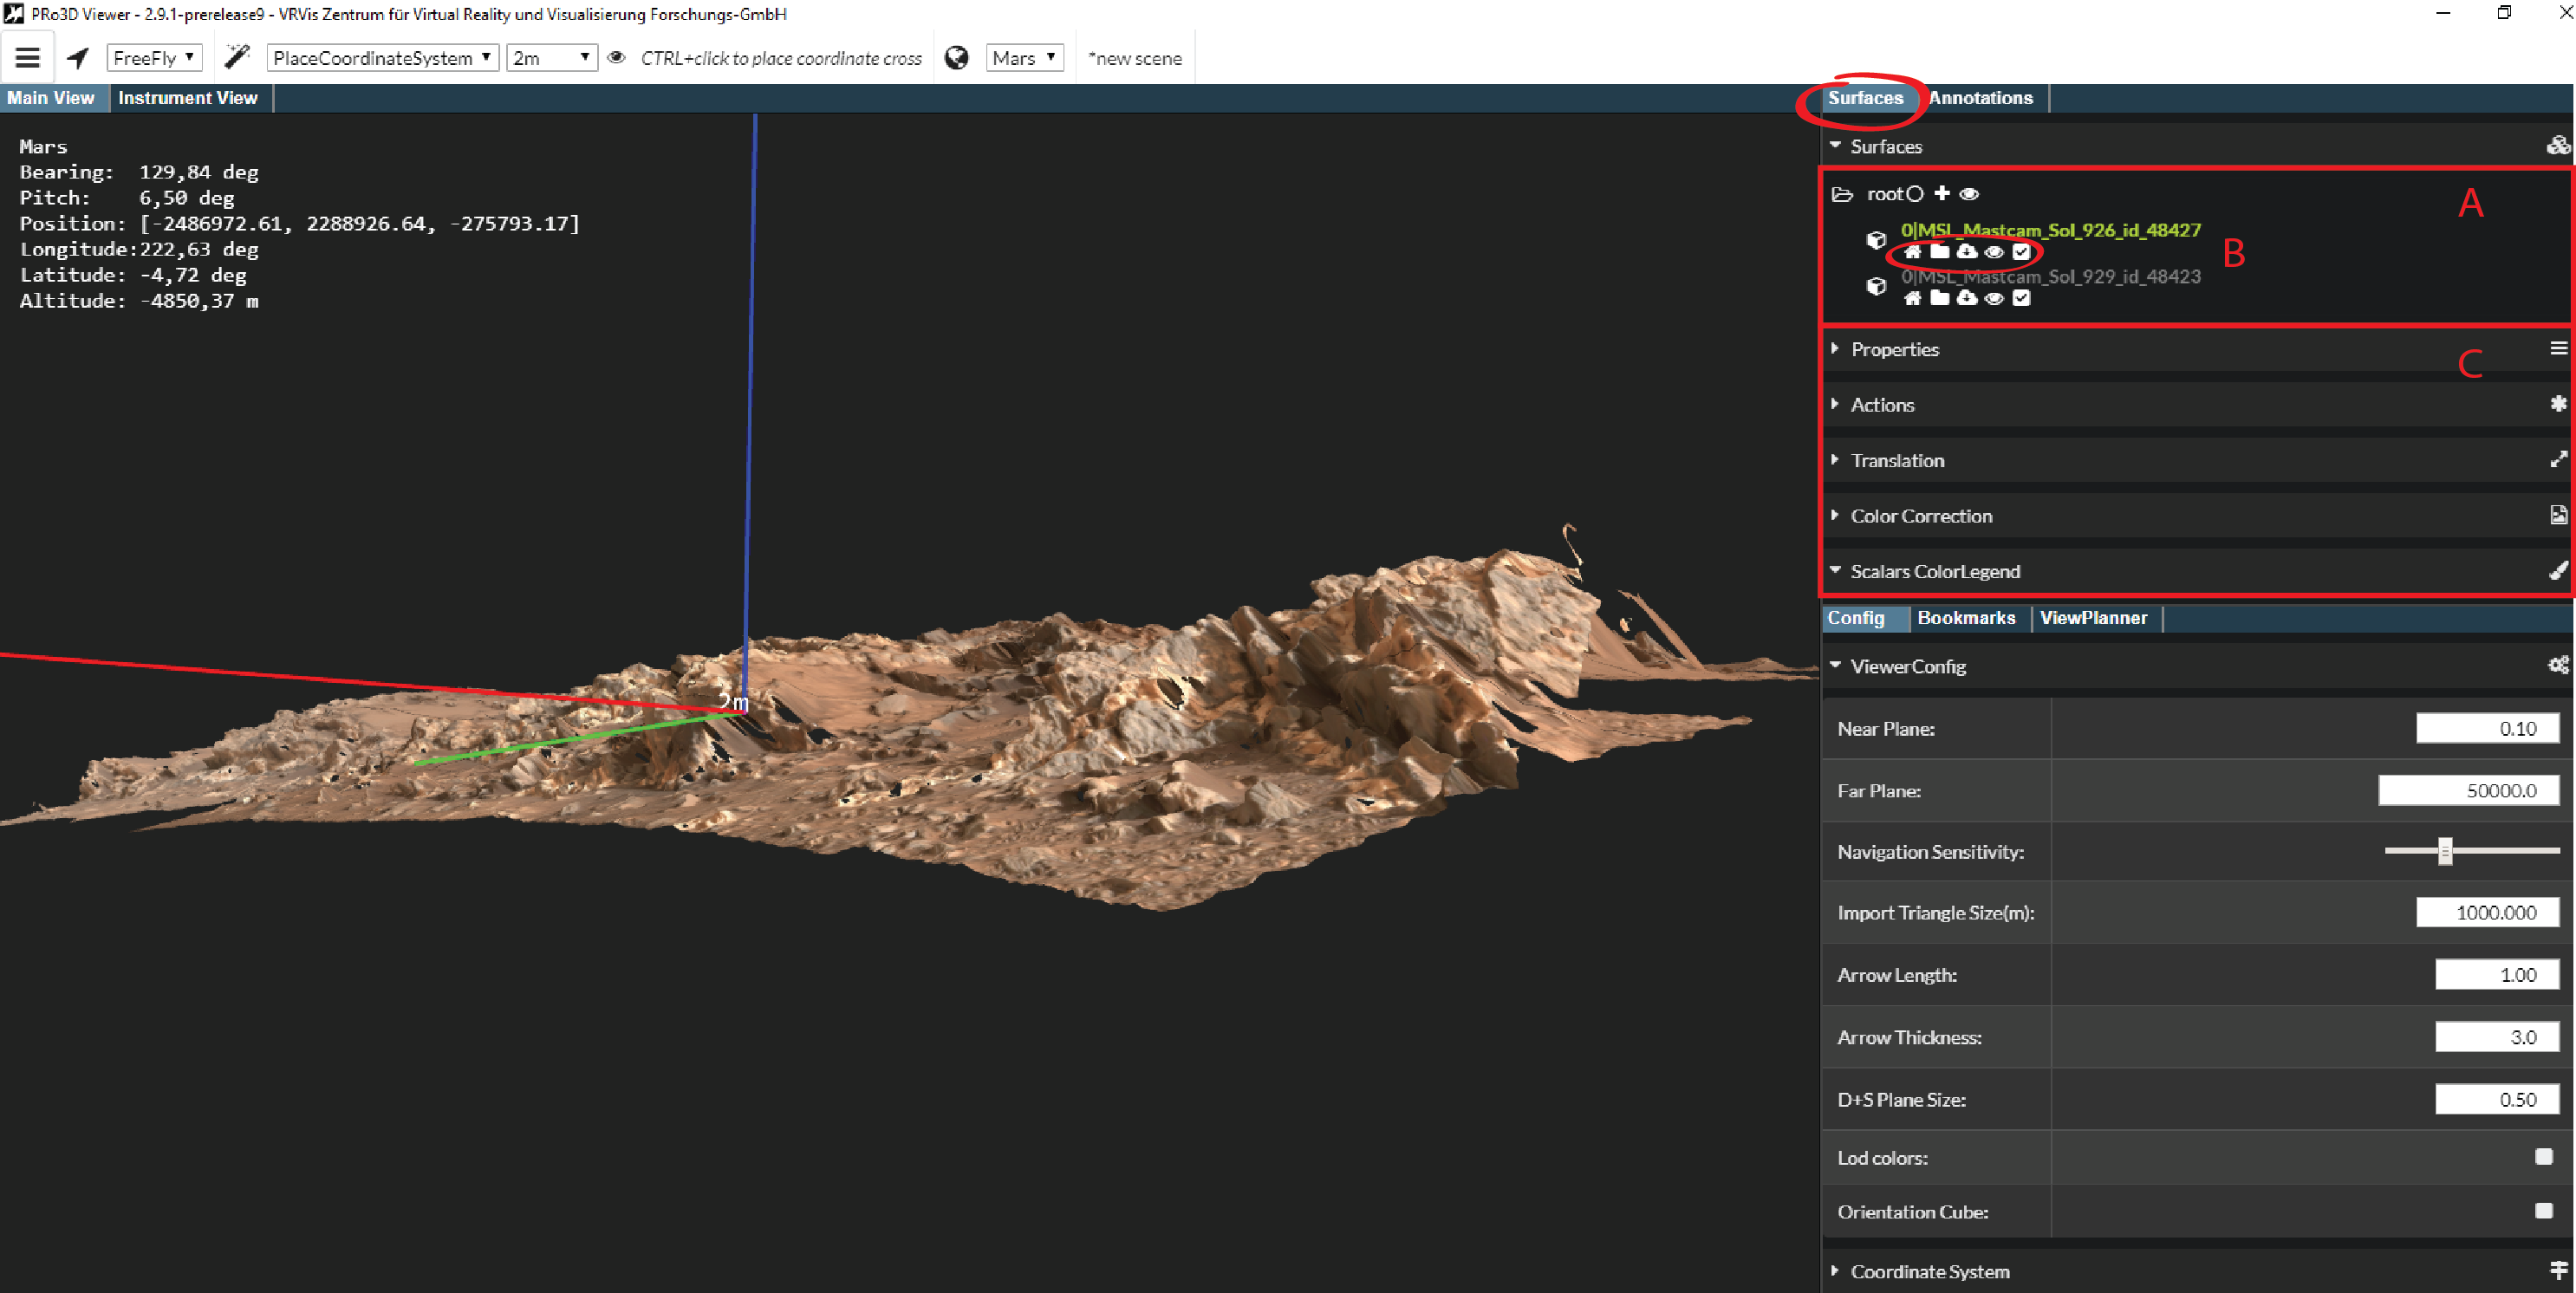
\includegraphics[width=1\textwidth]{pics/NewSurfaceAI.png}
    	\caption[New Surface]{Loaded surface with open surface features (right).}
    	\label{fig:NewSurface}
   \end{figure} 
	
%----------------------------------------------------------------------------------------
%	Section: Viewer Actions
%----------------------------------------------------------------------------------------
%----------------------------------------------------------------------------------------
%	Section: Viewer Actions
%----------------------------------------------------------------------------------------
\section{Viewer Actions}

\begin{figure}[h]
    	\centering
    		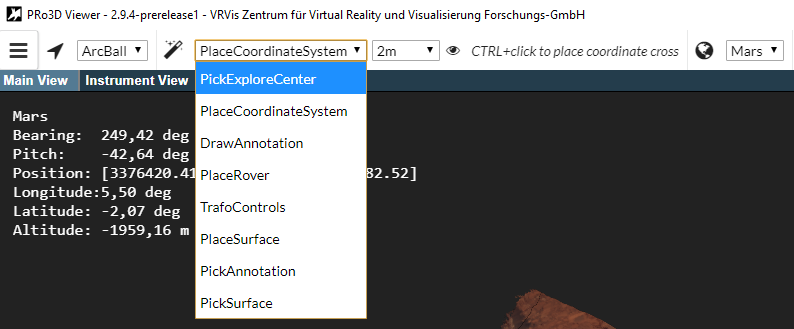
\includegraphics[width=1\textwidth]{pics/Interactions.png}
    	\caption[Interactions]{Viewer Actions.}
    	\label{fig:Interactions}
   \end{figure}

Once the surface is loaded there are different actions to choose (Figure~\ref{fig:Interactions}).
%----------------------------------------------------------------------------------------
%	SubSection: Pick Explore Center
%----------------------------------------------------------------------------------------
\subsection{Pick Explore Center}
\label{sec:pickEC}

The ``PickExploreCenter'' action concerns the \textbf{ArcBall} navigation mode. There are two navigation modes (Figure~\ref{fig:exploreCenter}):
\begin{itemize}
	\item \textbf{FreeFly} and 
	\item \textbf{ArcBall}.
\end{itemize}

\begin{figure}[h]
    	\centering
    		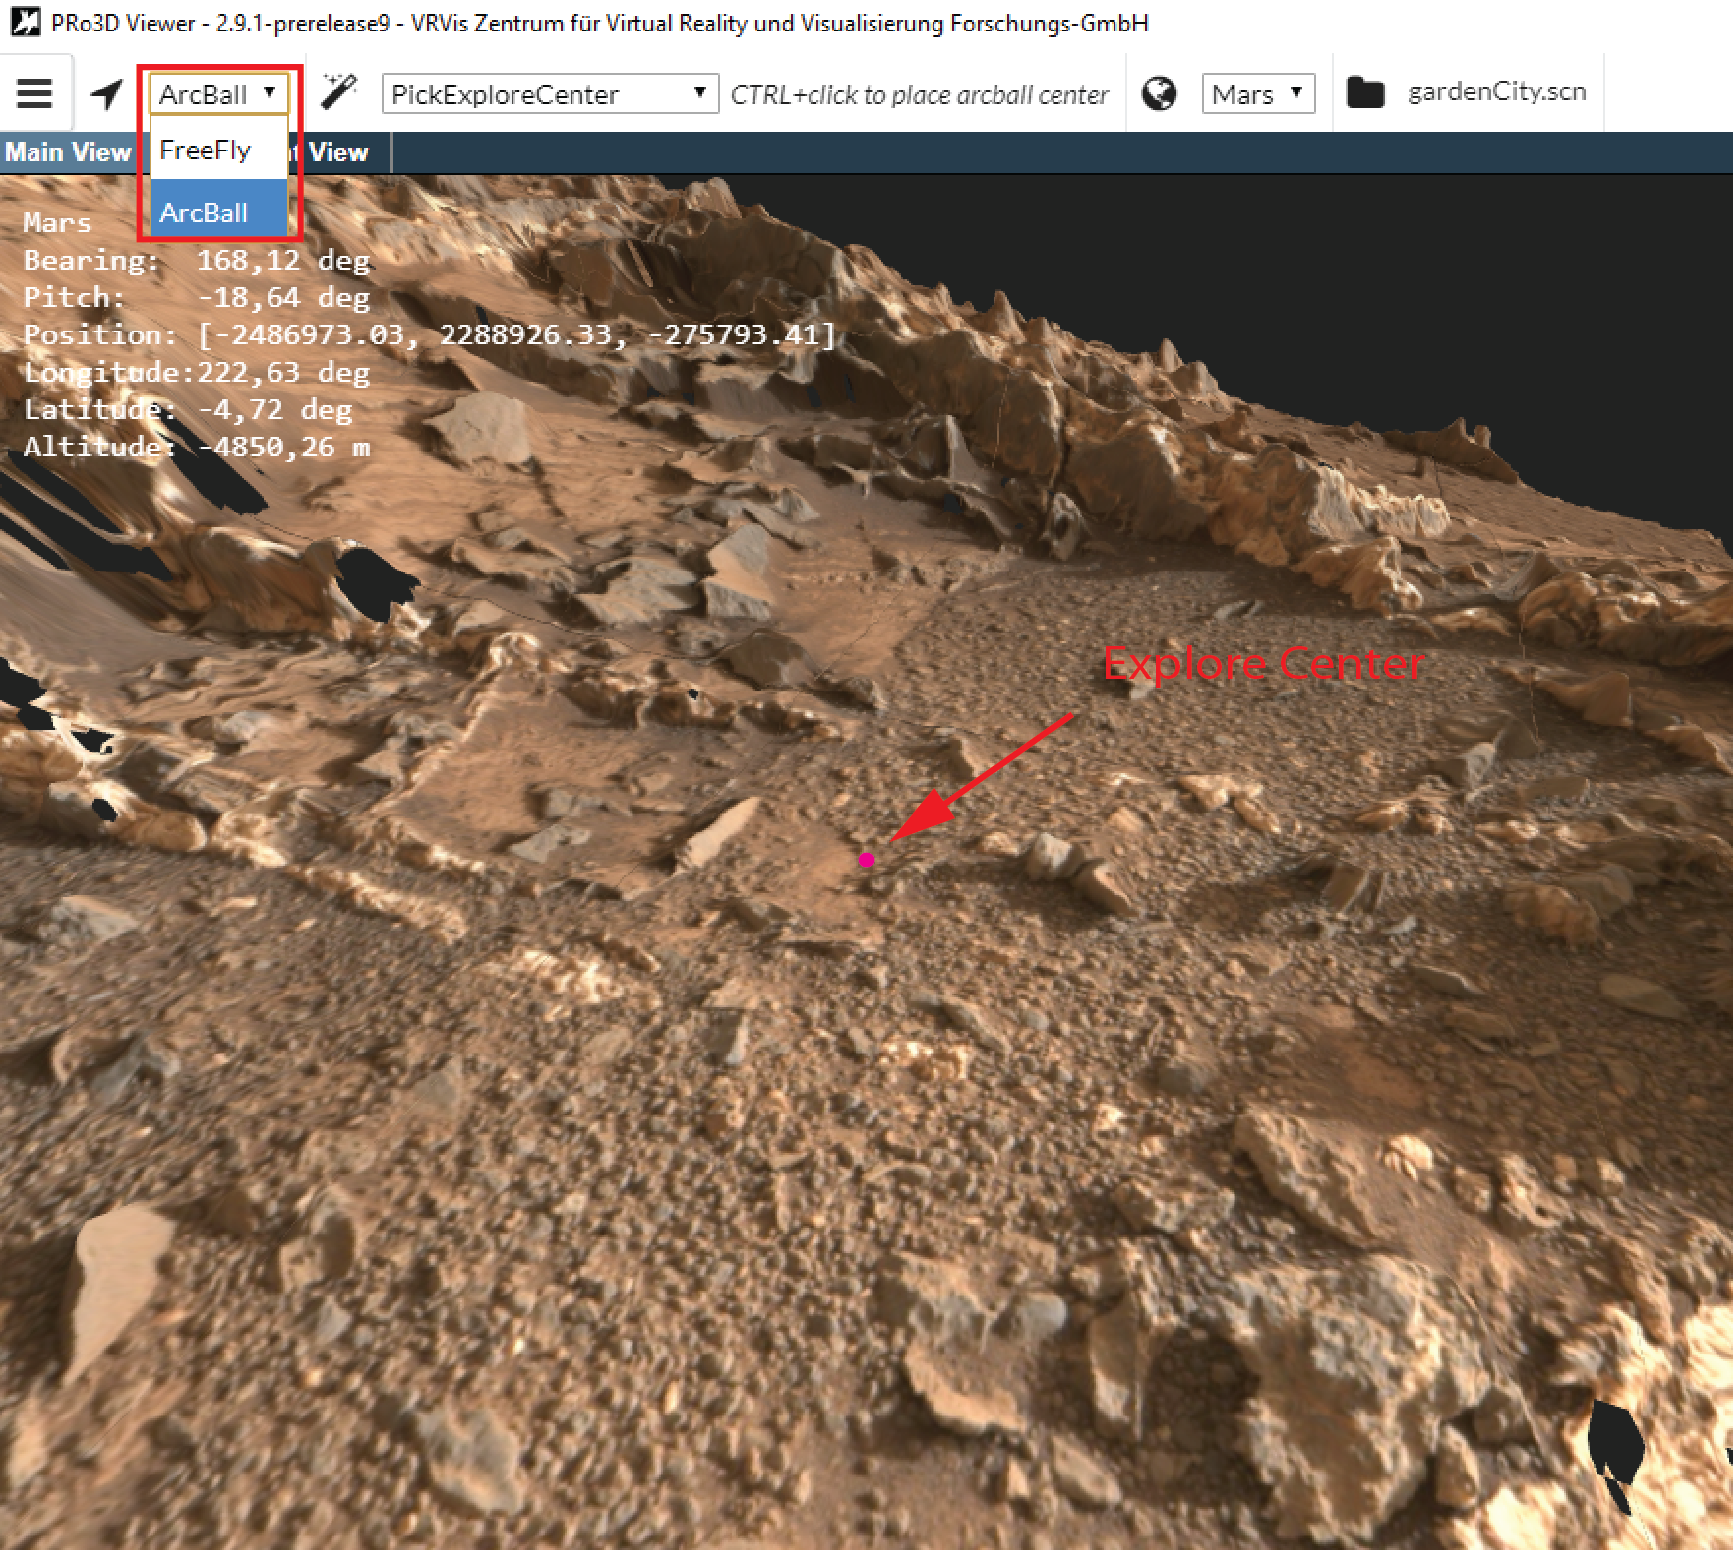
\includegraphics[width=1\textwidth]{pics/exploreCenterAI.png}
    	\caption[ExploreCenter]{ArcBall navigation. Explore center is set with CTRL + LMB and indicated by a pink dot.}
    	\label{fig:exploreCenter}
   \end{figure}

%----------------------------------------------------------------------------------------Free Fly-
\subsubsection{FreeFly}

The Free Fly Mode is the standard 3D fly-through navigation, as for instance, in terrain visualization. WASD controls forward/backward and strafing movement, while the user can change the camera's orientation by holding the LMB (= \textbf{L}eft \textbf{M}ouse \textbf{B}utton). Zooming in and out (forward/backward movement) is performed by turning the mouse-wheel or holding down the RMB (= \textbf{R}ight \textbf{M}ouse \textbf{B}utton). Additionally, the camera can be panned by holding down the middle mouse button.

%----------------------------------------------------------------------------------------Arc Ball-
\subsubsection{ArcBall}

When the viewer is in ArcBall mode the camera can be rotated around the explore center by holding down the LMB. Panning and strafing are possible as described above, but be aware that this moves the explore center (otherwise panning would break the view matrix of the camera). To set a new explore point, make sure the ``PickExploreCenter'' action is active (as shown in Figure~\ref{fig:exploreCenter}) and press CTRL + LMB on the surface. The explore center is indicated by a pink dot. Forward and backward movement is performed either by the keys W/S, rotating the mouse wheel, or clicking the RMB.
%----------------------------------------------------------------------------------------
%	SubSection: Place Coordinate System
%----------------------------------------------------------------------------------------
\subsection{Place Coordinate System}
\label{sec:placeCS}

\begin{figure}[h]
    	\centering
    		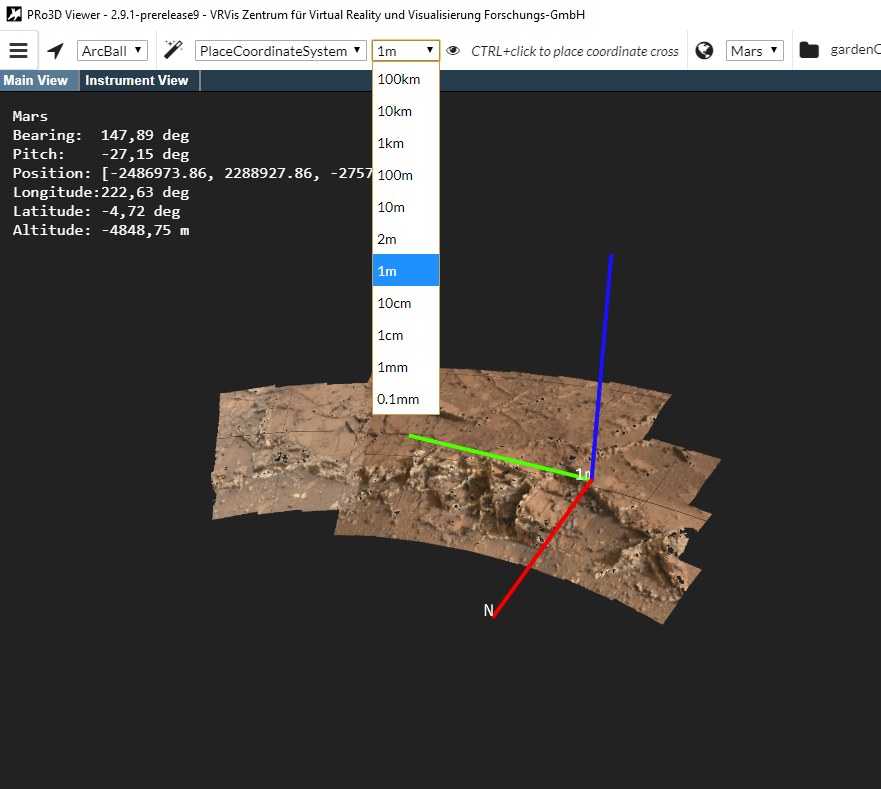
\includegraphics[width=1\textwidth]{pics/CoordinateSystem.png}
    	\caption[Coordinate System]{Coordinate System with scale bar functionality.}
    	\label{fig:coordinateSystem}
   \end{figure}
	
To set the coordinate system pick ``PlaceCoordinateSystem'' in the actions drop down menu, select a unit of measurement and press CTRL+LMB to pick a point on the surface. This marks the position as shown in Figure~\ref{fig:coordinateSystem}.
Initially the up vector's (blue) direction is set in the positive z-direction and the north vector's (red) in the positive y-direction. You can manipulate the north vector manually for different data. The surface can be translated along the three directions of the coordinate system, as described in Section~\ref{sec:surfaces}. The up- and the north vector are used for the projection measurements. The north vector is also relevant for bearing measurements, and the rover placement in the View Planner.
%(see Section~\ref{sec:viewPlanner})
The value for manipulating the north vector is shown in the Viewer Configuration described in Section~\ref{sec:config}.
%----------------------------------------------------------------------------------------
%	SubSection: Draw Annotation
%----------------------------------------------------------------------------------------
\subsection{Draw Annotation}
\label{sec:drawAnnotation}

\begin{figure}[h]
    	\centering
    		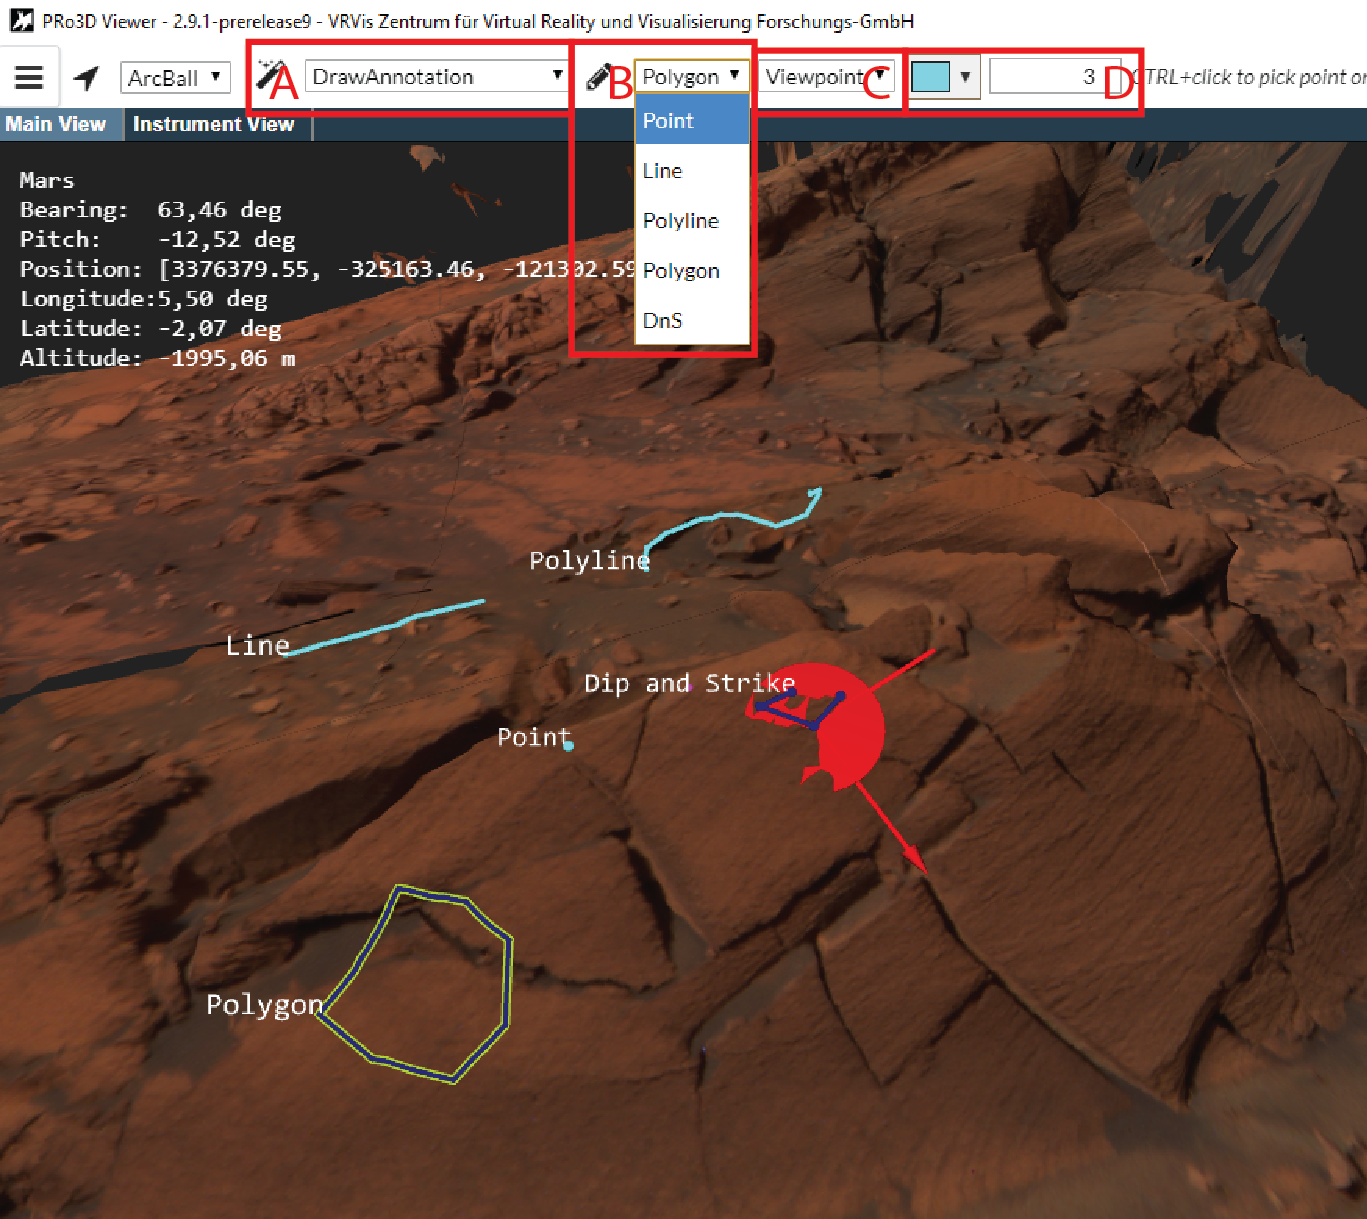
\includegraphics[width=1\textwidth]{pics/drawAnnotationsAI.png}
    	\caption[Draw Annotations]{Annotation settings: \textbf{A}: set viewer action to ``DrawAnnotation. \textbf{B}: select annotation mode. \textbf{C}: select projection. \textbf{D}: choose color and thickness. }
    	\label{fig:drawAnnotations}
   \end{figure}
	
Figure~\ref{fig:drawAnnotations} shows the settings for drawing annotations. First set ``DrawAnnotation'' in the actions menu (A in Figure~\ref{fig:drawAnnotations}). Then you can choose one of the following annotation modes (B in Figure~\ref{fig:drawAnnotations}):
\begin{itemize}
	\item \textit{Point}: A single point measurement on the surface.
	\item \textit{Line}: You can pick two points on the surface. The connecting line depends on the projection mode explained in the table below.
	\item \textit{Polyline}: An arbitrary number of points on the surface can be picked. The connecting line segments depend on the projection mode. The polyline is finished by pressing Enter.
	\item \textit{Polygon}: An arbitrary number of points on the surface can be picked. The connecting line segments depend on the projection mode. The region of interest is closed and finished by pressing Enter.
	\item \textit{DnS}: (\textit{= Dip and Strike}) A polyline onto a surface, e.g. alongside a rock layer can be picked. After clicking Enter, a plane is fitted (least squares) to this polyline (blue), which is then intersected with a horizontal plane, which gives us the so-called strike vector (red). This vector represents the direction within the plane with the least inclination and orthogonal to it is the dip vector (green) which shows the direction of highest inclination as shown in Figure~\ref{fig:drawAnnotations}.
\end{itemize}
To pick an annotation point on the surface press CTRL+LMB.

For all annotations (except Point) you can choose between ``Linear'', ``ViewPoint'' and ``Sky'' projection which determines the direction of the picking ray (C in Figure~\ref{fig:drawAnnotations}):
\begin{itemize}
	\item \textit{Linear}: produces straight line segments as point-to-point connections with linear interpolation between them, no actual projection is performed (Figure~\ref{fig:projection}, blue line). This is useful for line-of-flight distance measurements or measuring the height of a cliff or determining its slope.
	\item \textit{ViewPoint}: between two points we sample the space by shooting additional rays to intersect with the surface, in this case along the view direction (Figure~\ref{fig:projection}, green line). This is helpful to measure details in nooks and crannies of a rough surface and is the typical way to go for geological measurements.
	\item \textit{Sky}: the same sampling happens as for the viewpoint projection but this time the rays are shot along the scene's up-vector (Figure~\ref{fig:projection}, pink line). This mode is useful for geographical measurements to estimate the length of a path through a crater.
\end{itemize}

\begin{figure}[h]
    	\centering
    		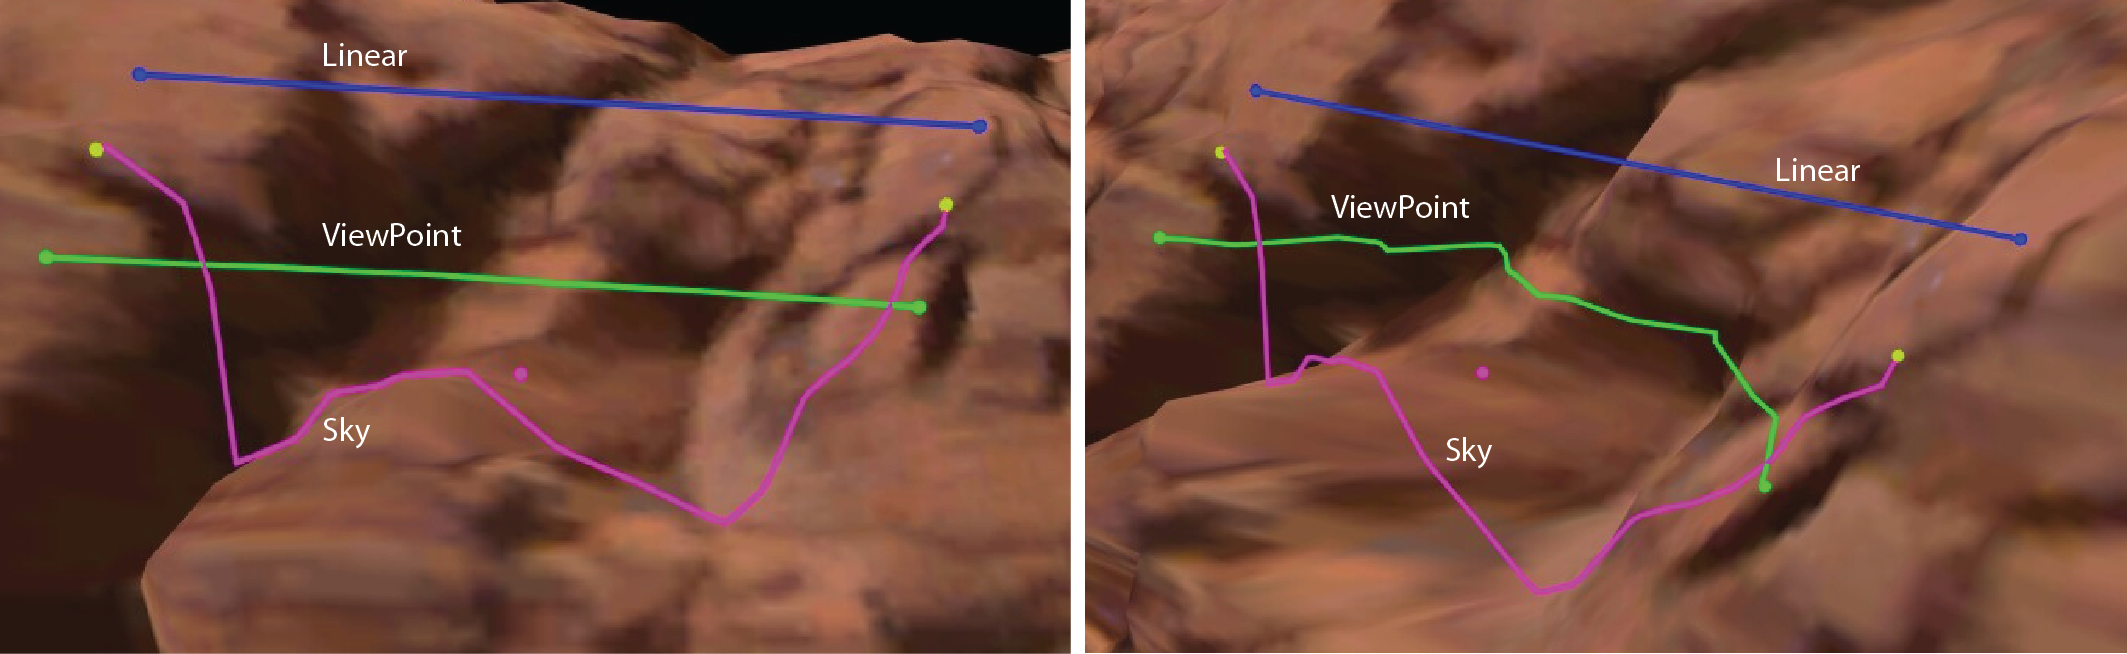
\includegraphics[width=1\textwidth]{pics/projectionAI.png}
    	\caption[Projections]{Three Lines taken from the same camera position (left) with the same camera settings but with different line projections.}
    	\label{fig:projection}
   \end{figure}
	
Finally you can set the color and thickness of the annotation (D in Figure~\ref{fig:drawAnnotations}).
Section~\ref{sec:annotations} shows how to maintain, group and edit existing annotations.

%----------------------------------------------------------------------------------------
%	SubSection: Pick Annotation
%----------------------------------------------------------------------------------------
\subsection{Pick Annotation}
\label{sec:pickAnnotation}

There are two ways to select an annotation:

\begin{enumerate}
	\item You can select an annotation by clicking on the annotation's name in the annotation's listing described in Section~\ref{sec:annotations}.
	\item Or you set ``PickAnnotation'' in the actions menu, press CTRL+LMB and pick the annotation in the main view.
\end{enumerate}
Then the annotation turns its color to green in the listing and gets a green border in the main view as shown in Figure~\ref{fig:drawAnnotations}, where the Polygon is selected. Once selected, you can explore and adjust the annotation's properties (see Section~\ref{sec:annotations}).
%----------------------------------------------------------------------------------------
%	SubSection: Pick Surface
%----------------------------------------------------------------------------------------
\subsection{Pick Surface}
\label{sec:pickSurface}

There are two ways to select a surface:

\begin{enumerate}
	\item You can select a surface by clicking on the surface's name in the surface's listing described in Section~\ref{sec:surfaces}.
	\item Or you set ``PickSurface'' in the actions menu, press CTRL+LMB and pick the surface in the main view.
\end{enumerate}
Then the surface's name turns its color to green in the listing. Once selected, you can explore and adjust the surface's properties (see Section~\ref{sec:surfaces}).

%----------------------------------------------------------------------------------------
%	SubSection: Place Rover
%----------------------------------------------------------------------------------------
%\subsection{Place Rover}
%\label{sec:placeRover}

%----------------------------------------------------------------------------------------
%	SubSection: Trafo Controls
%----------------------------------------------------------------------------------------
%\subsection{Trafo Controls}
%\label{sec:trafoControls}

%----------------------------------------------------------------------------------------
%	SubSection: Align Pick
%----------------------------------------------------------------------------------------
%\subsection{Align Pick}
%\label{sec:alignPick}


%----------------------------------------------------------------------------------------
%	Section: Viewer Features
%----------------------------------------------------------------------------------------
%----------------------------------------------------------------------------------------
%	Section: Viewer Features
%----------------------------------------------------------------------------------------
\section{Viewer Features}

\begin{figure}[h]
    	\centering
    		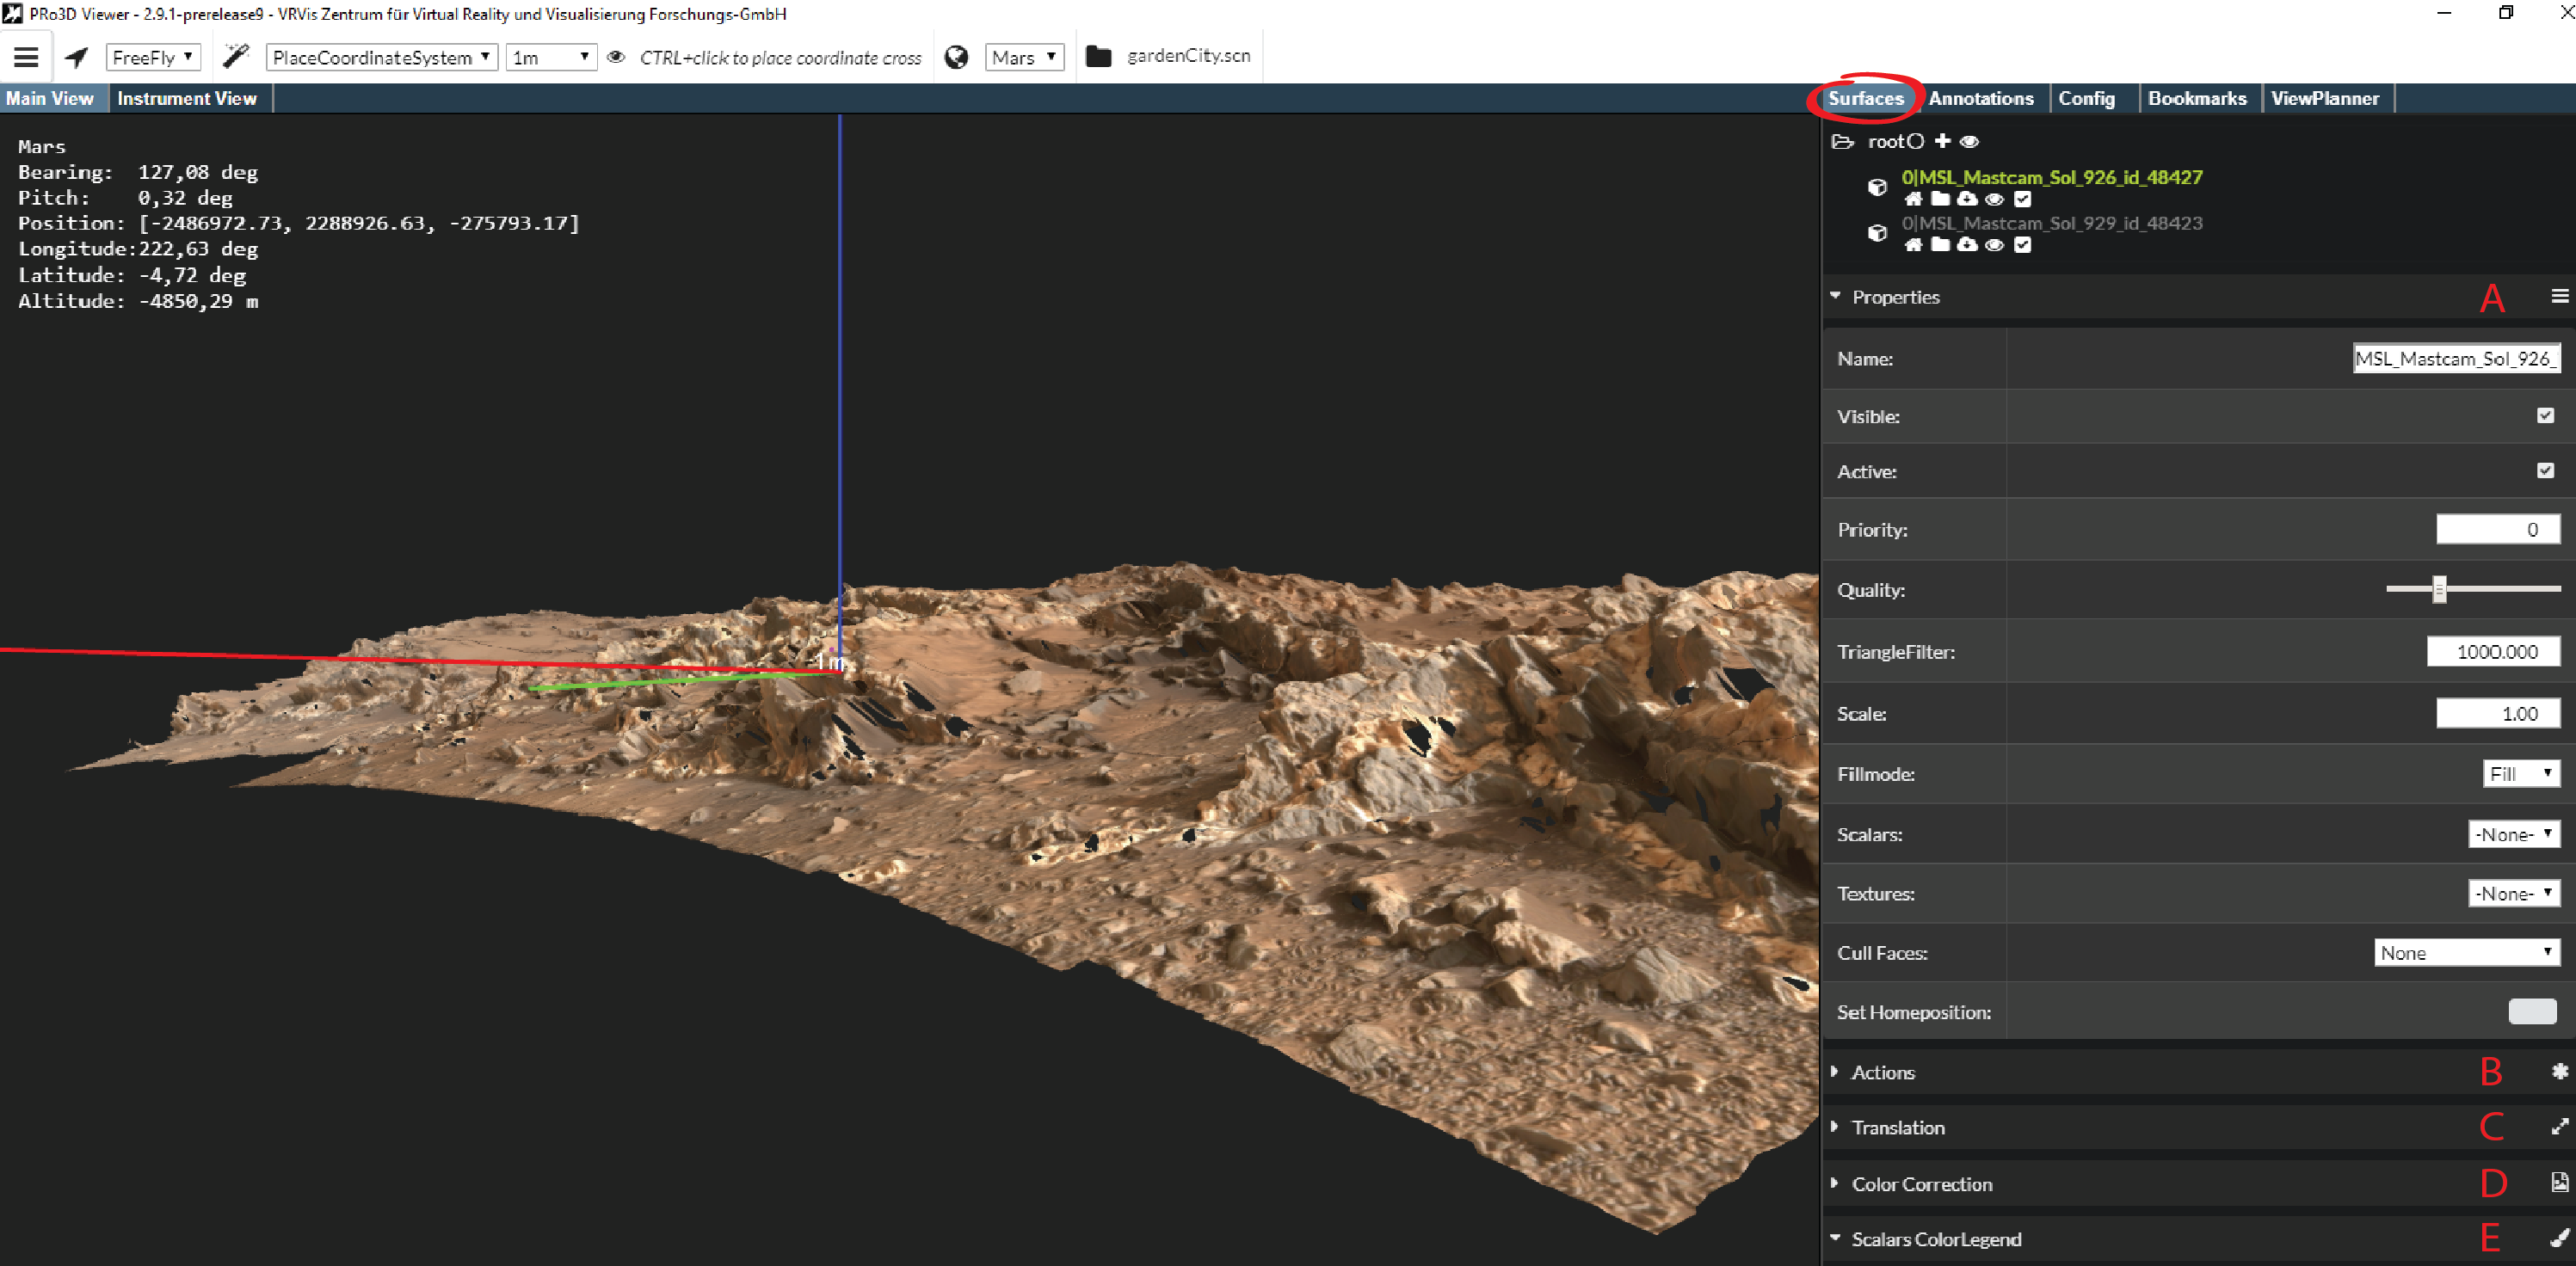
\includegraphics[width=1\textwidth]{pics/SurfacesAI.png}
    	\caption[Viewer Features]{There are pages (right) for each feature in the viewer.}
    	\label{fig:featureMenu}
   \end{figure}
	
The feature pages show a list of the respective features, the properties of the selected feature from this list, and some actions for this feature.
For surfaces, annotations, and bookmarks it is possible to group them, as described in Section~\ref{sec:grouping}.
%----------------------------------------------------------------------------------------
%	SubSection: Surfaces
%----------------------------------------------------------------------------------------
\subsection{Surfaces}
\label{sec:surfaces}

The listing shows all surfaces in the scene. You can classify them in any group and subgroup layers, described in Section~\ref{sec:grouping}.
You can select a surface by clicking on the surface's name, which turns its color to green. Or you can set ``PickSurface'' in the actions menu (Figure~\ref{fig:Interactions}), press CTRL+LMB and pick the surface in the main view. Then you can see the surface's properties in the properties panel and use the actions in the actions panel. 
It is also possible to select multiple surfaces by clicking the square icon in front of each surface. The selected surfaces have a green square in the list. The multiselection is used to move one ore more surfaces from one group to the active group.
Under the surface's name is a little menu:
\begin{itemize}
	\item \textit{FlyTo}: A click on the button triggers a FlyTo animation.
	\item \textit{openFolder}: Opens the folder where the scene file resides.	
	\item \textit{Cloud}: Creates new kd-tree files.	
	%\item \textit{portable}: This creates a folder hierarchy as used in the old viewer version. A scene file is created and the surfaces are
  %copied to the surface folder.
	\item \textit{Toggle Visible}: Toggles the surface visible/invisible.	
	\item \textit{Toggle IsActice}: You can only pick on active surfaces (explore center, annotations, ...).
	
\end{itemize}

\begin{figure}[h]
    	\centering
    		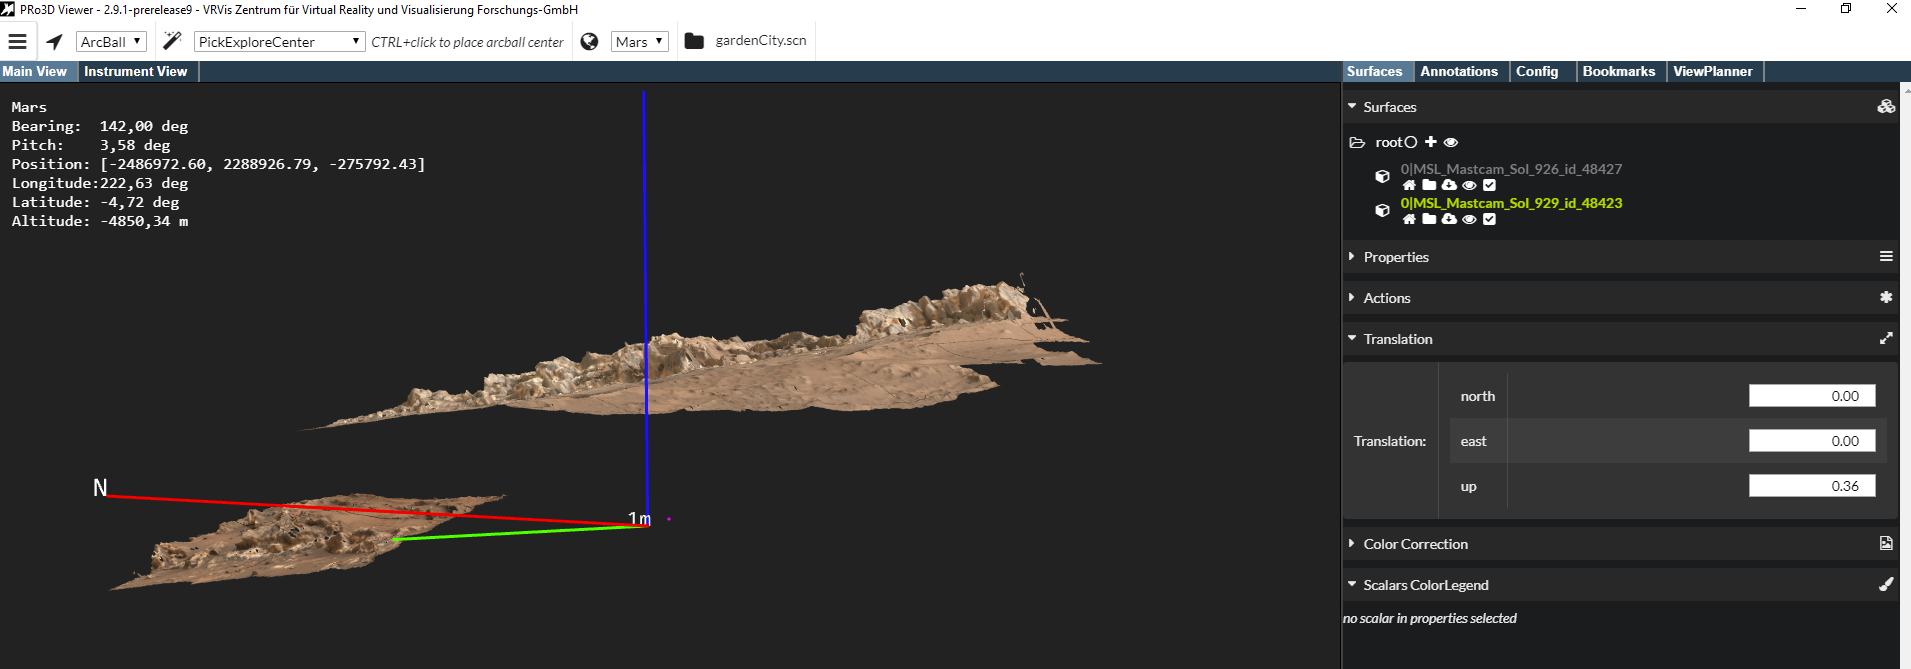
\includegraphics[width=1\textwidth]{pics/SurfaceTranslation.png}
    	\caption[Surface Translation]{Translation of the selected surface along the axes of the coordinate system.}
    	\label{fig:surfaceTranslation}
   \end{figure}

For each selected surface there are several panels as shown in Figure~\ref{fig:featureMenu} A to E. 

In the surface properties panel (Figure~\ref{fig:featureMenu} A) some adjustments are possible:
\begin{itemize}
	\item \textit{Name}: The surface's name. You can change it in the text field and press ``enter''.
	\item \textit{Visible}: The surface is visible (checked) or not (unchecked).
	\item \textit{Active}: The surface is active (checked) or not (unchecked). You can only pick on active surfaces.
	\item \textit{Priority}:  Often multiple surfaces are available for a certain area on the planet surface. These surfaces represent the same piece of ground and typically overlap. This parameter allows you to assign a priority to a surface to tell the graphics card which surface should be rendered in front. Lower numbers mean a higher priority in rendering, with 0 being the highest priority. You can also give the highest priority surface a ranking of, for instance, 0.1 (= 10cm) to make annotations more visible. The priority can be dynamically changed via the surface properties so you can try out what works best.
	\item \textit{Quality}: 
	\item \textit{TriangleFilter}: Excludes triangles with edges bigger than the entered value.
	\item \textit{Scale}: 
	\item \textit{FillMode}: You can switch between solid/ wireframe/ point rendering of the geometry.
	\item \textit{Scalars}: Select an attribute layer.
	\item \textit{Textures}: Select a texture layer.
	\item \textit{Cull Faces}:
	\item \textit{Set Homeposition}: You set a new camera position for FlyTo.
\end{itemize}

The surfaces actions (Figure~\ref{fig:featureMenu} B) are described in Section~\ref{sec:leafActions}. \\


You can translate the surface along the north-, east and up axis of the coordinate system, described in Section~\ref{sec:placeCS}. And you can rotate the surface around the up vector of the coordinate system. The Translation panel is shown in Figure~\ref{fig:featureMenu} B and Figure~\ref{fig:surfaceTranslation}. \\

\begin{center}
\colorbox{red}{\parbox{1.0\textwidth}{NOTE: Translation and Rotation only work for surfaces. Annotations, Rovers, the Coordinate System, etc. will NOT move with the surface. You have to transform the surface first!}}
\end{center}

\begin{figure}[h]
    	\centering
    		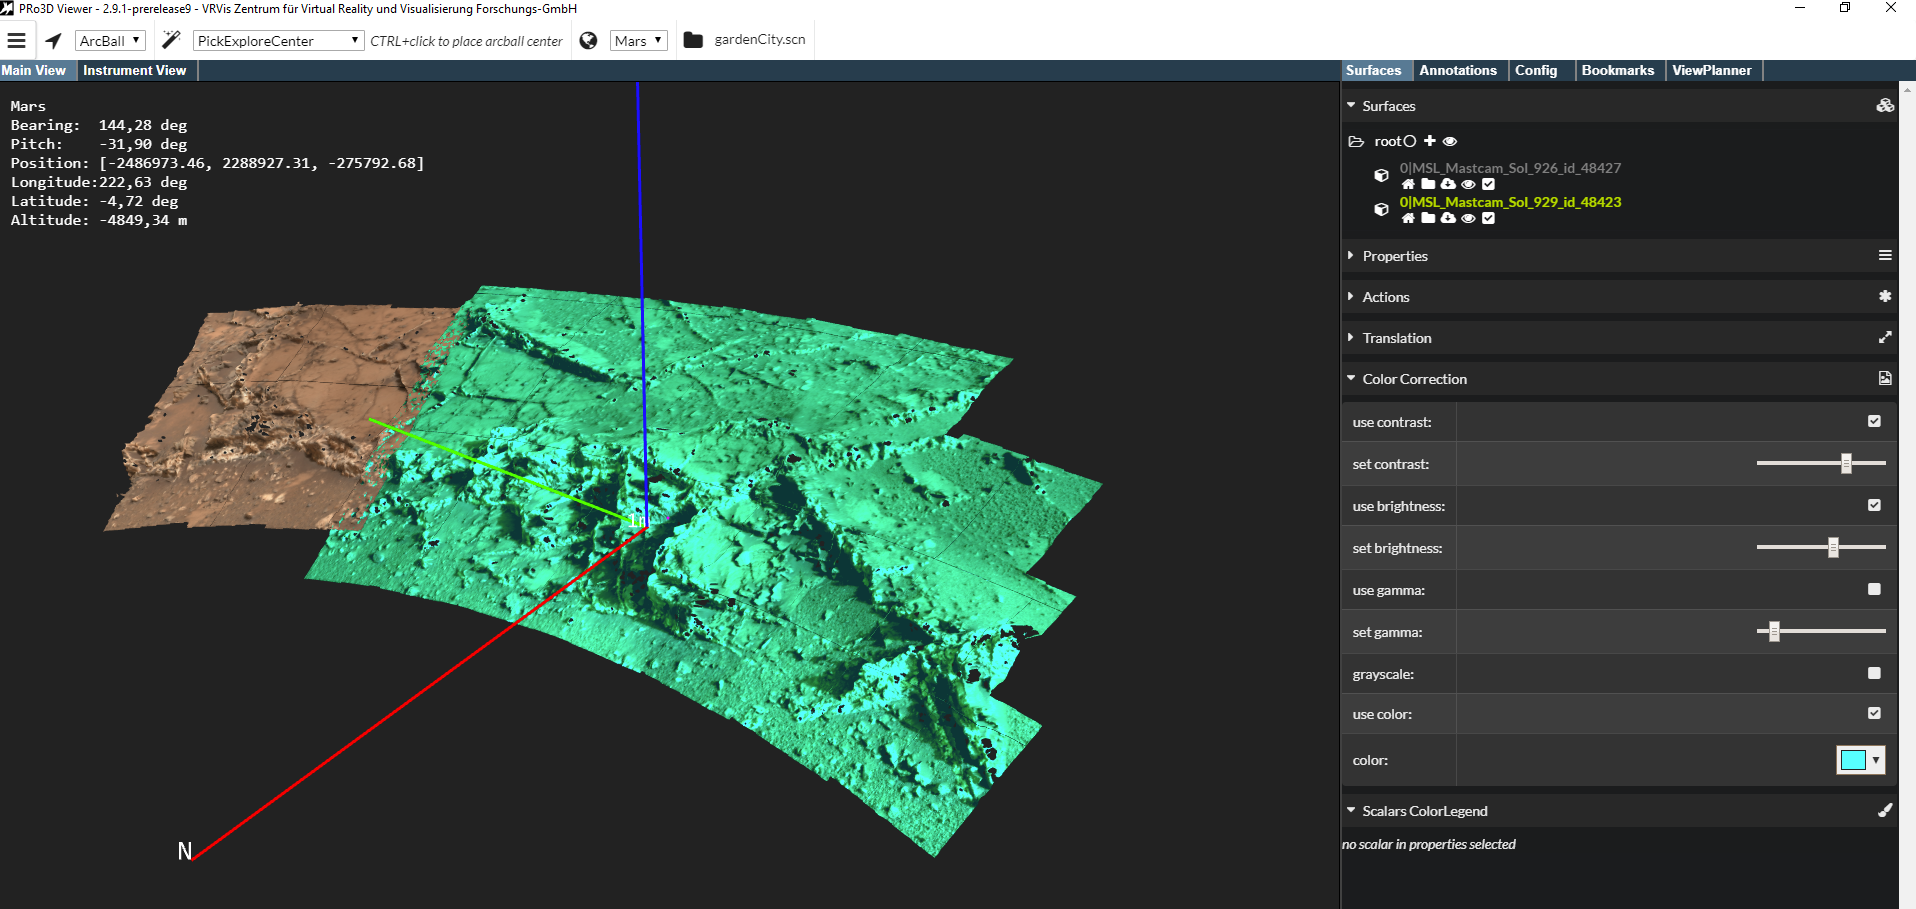
\includegraphics[width=1\textwidth]{pics/SurfaceColorCorrection.png}
    	\caption[Surface Color Correction]{Contrast-, brightness- and color filters applied on the selected surface.}
    	\label{fig:surfaceColorCorrection}
   \end{figure}

You can apply different color correction filters on the selected surface	(Figure~\ref{fig:surfaceColorCorrection}). \\

\begin{figure}[h]
    	\centering
    		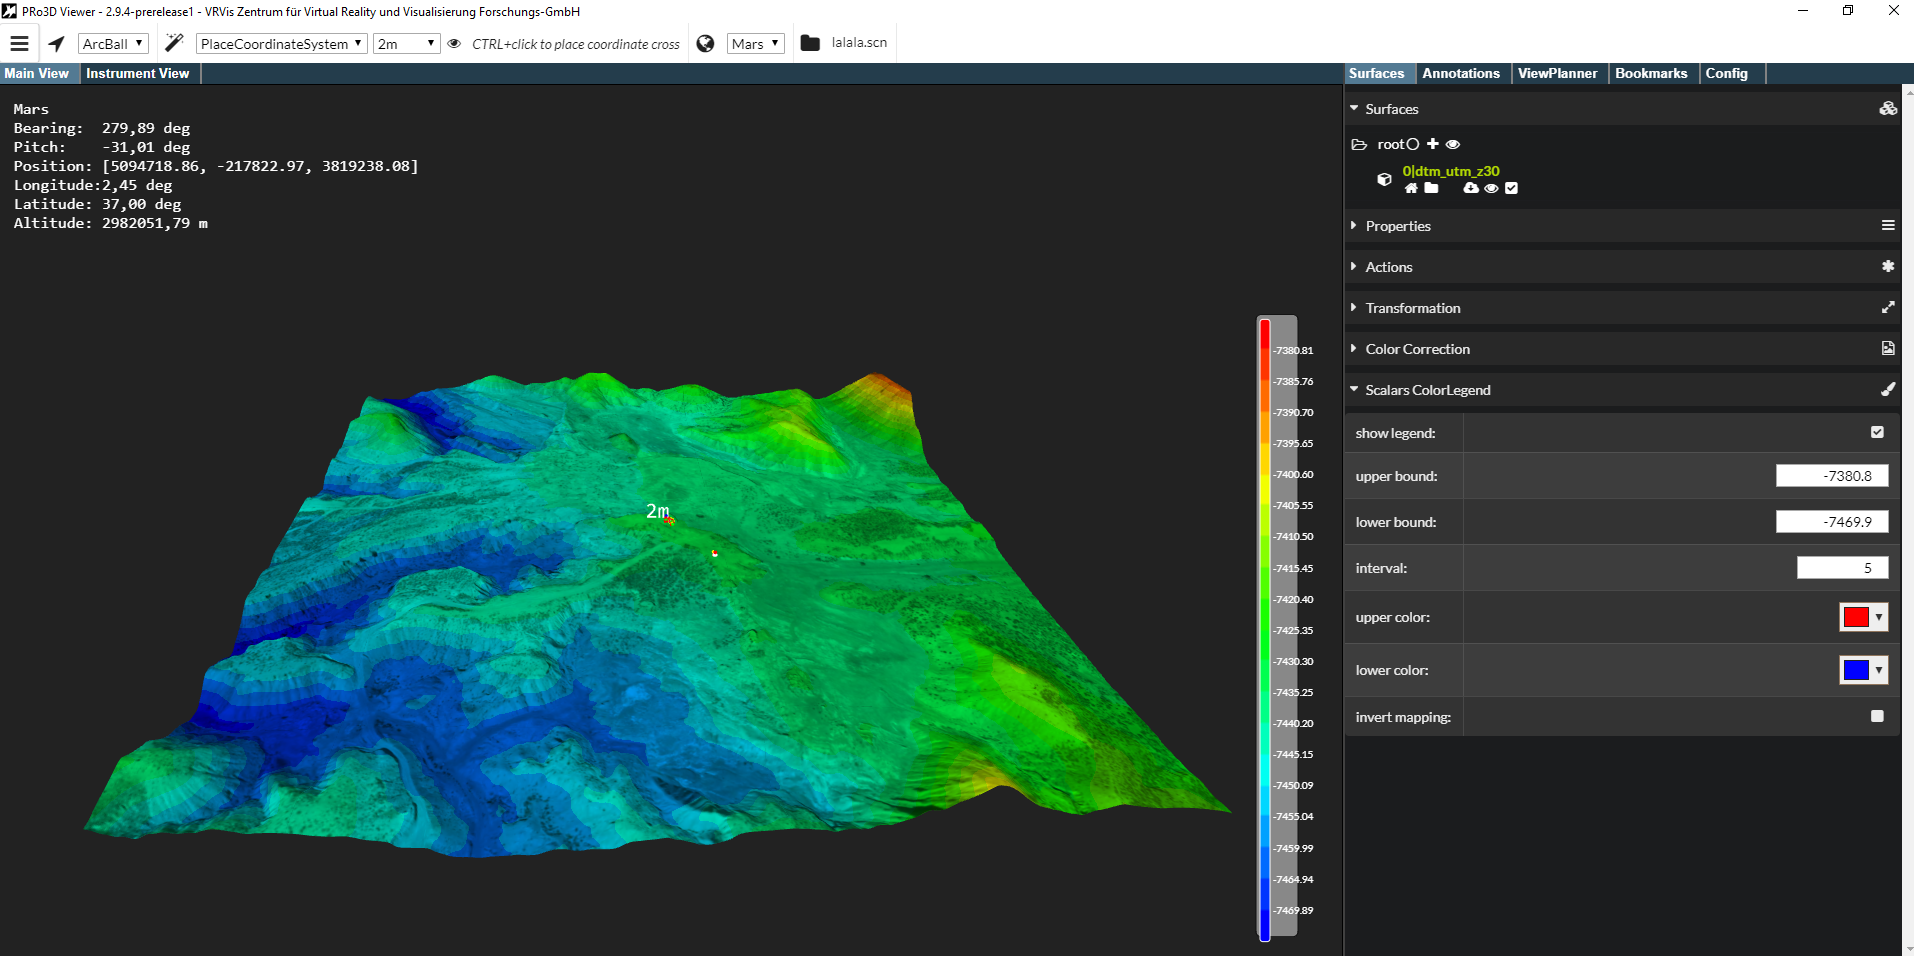
\includegraphics[width=1\textwidth]{pics/SurfaceColorLegend.png}
    	\caption[Surface Color Legend]{A height map visualized by false color mapping.}
    	\label{fig:surfaceColorLegend}
   \end{figure}
	
Within the effort of including more and more meta data for a surface we included the so-called SurfaceAttributes (see Figure~\ref{fig:surfaceColorLegend}),
which are specified in an .opcx file carrying the name of the respective surface.
For now, these surface attributes mainly contain additional layers, which can either be a texture layer or an attribute layer.
Texture layers are just alternative texture maps that can be mapped onto the surface, such as images from different filters or even sensors (spectral image). 
Attribute maps on the other hand present an additional value for each position of a surface. 
If a surface has an .opcx file attached its layers are listed and can be selected in the \textit{Scalars} and the \textit{Textures} combo boxes as part of the surface's property control (Figure~\ref{fig:featureMenu}). 
In the Scalars ColorLegend panel, the color legend can be adjusted (Figure~\ref{fig:surfaceColorLegend}).

%----------------------------------------------------------------------------------------
%	SubSection: Annotations
%----------------------------------------------------------------------------------------
\newpage
\subsection{Annotations}
\label{sec:annotations}

\begin{figure}[h]
    	\centering
    		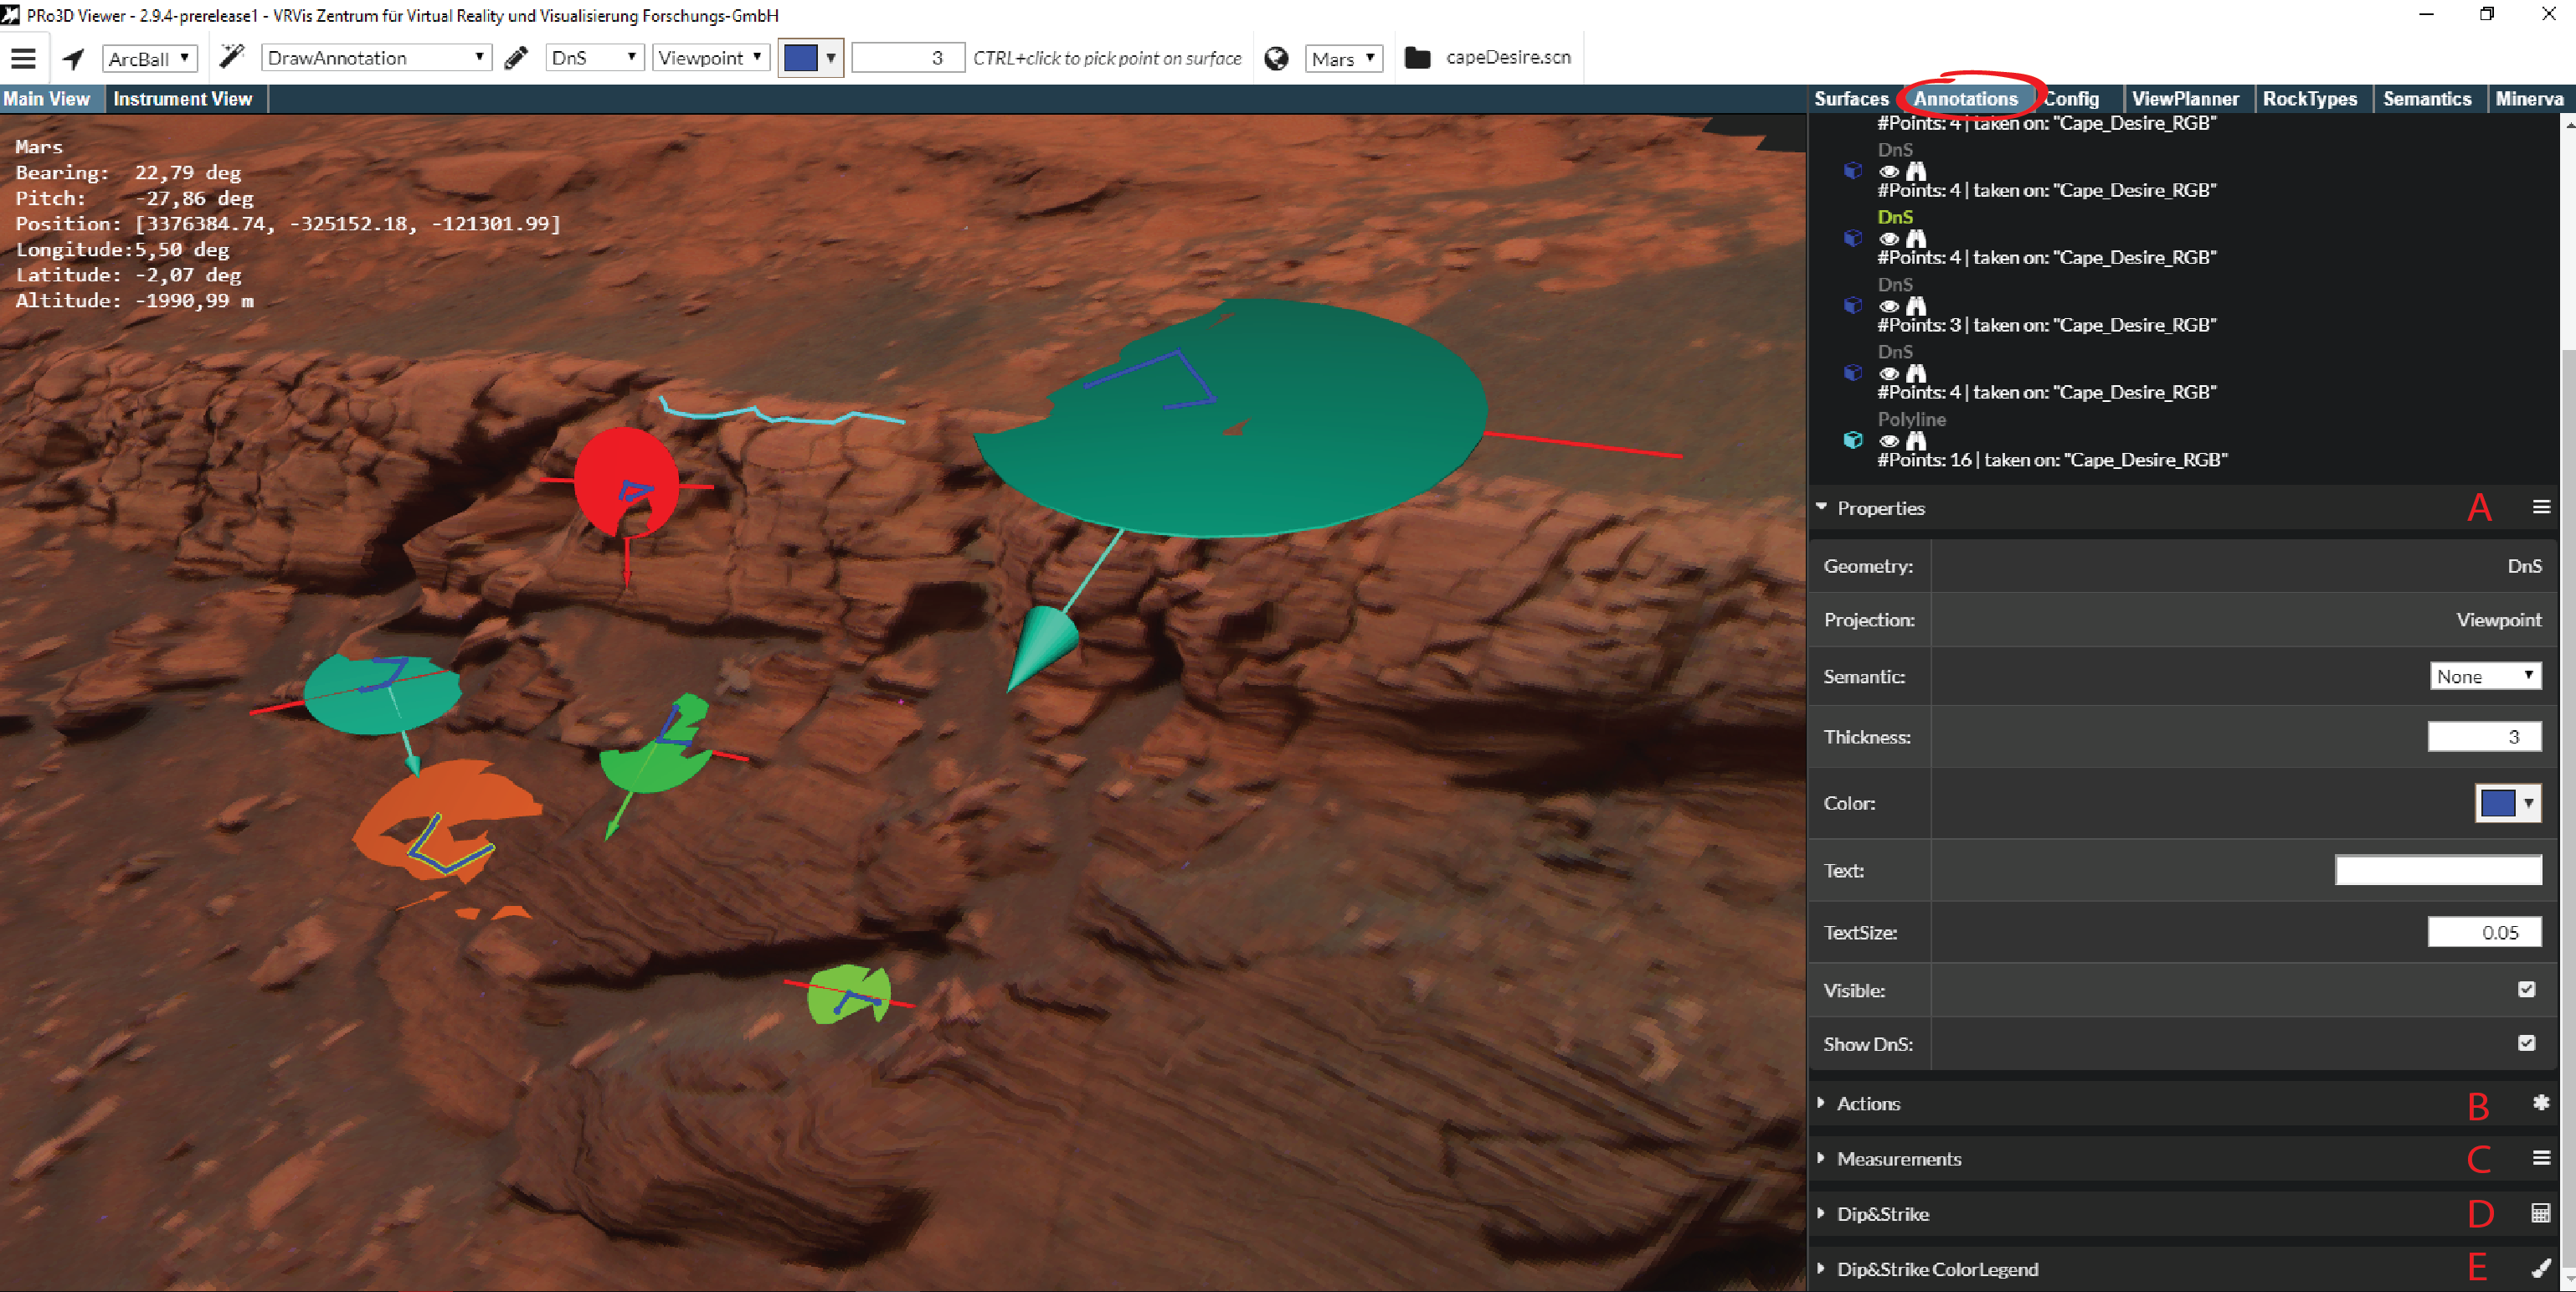
\includegraphics[width=1\textwidth]{pics/AnnotationsAI.png}
    	\caption[Viewer Features Annotations]{The annotations page.}
    	\label{fig:annoProps}
   \end{figure}
	
The listing shows all annotations in the scene. You can classify them in any group and subgroup layers, described in Section~\ref{sec:grouping}.
You can select an annotation by clicking on the annotation's name, which turns its color to green. Or you can set ``PickAnnotation'' in the actions menu (Figure~\ref{fig:Interactions}), press CTRL+LMB and pick the annotation in the main view. Then you can see the annotation's properties in the properties panel and use the actions in the actions panel. 
It is also possible to select multiple annotations by clicking the square icon in front of each annotation. The selected annotations have a green square in the list. The multiselection is used to move one ore more annotations from one group to the active group.\\
Under the annotation's name is a little menu:
\begin{itemize}
  \item \textit{Toggle}: Toggles the annotation visible/invisible.
	\item \textit{FlyTo}: A click on the button triggers a FlyTo animation.
\end{itemize}

For each selected annotation there are several panels as shown in Figure~\ref{fig:annoProps} A to E. 

The properties of the selected annotation (click on annotation's name) are shown in Figure~\ref{fig:annoProps} A. There you can get information and change some of the settings:
\begin{itemize}
	\item \textit{Geometry}: Shows the annotation mode (described in Section~\ref{sec:drawAnnotation}). This is not changeable retrospectively.
	\item \textit{Projection}: Shows the projection which determines the direction of the picking ray (described in Section~\ref{sec:drawAnnotation}, shown in Figure~\ref{fig:projection}). This is not changeable retrospectively.
	\item \textit{Semantic}: 
	\item \textit{Thickness}: You can change the annotation's line thickness.
	\item \textit{Color}: You can change the annotation's color.
	\item \textit{Text}: You can append a note. Write in the text field and press ``Enter''. The note will appear next to the annotation in the viewer. 
	\item \textit{TextSize}: You can change the textsize.
	\item \textit{Visible}: The annotation is visible (checked) or not (unchecked).
	\item \textit{ShowDnS}: For each annotation with more than three picking points Dip and Strike information (Section~\ref{sec:drawAnnotation}) is available. The DnS is visible (checked) or not (unchecked).
\end{itemize}

The annotations actions (Figure~\ref{fig:annoProps} B) are described in Section~\ref{sec:leafActions}.\\

The measurements tab (Figure~\ref{fig:annoProps} C) contains some information:
\begin{itemize}
	\item \textit{Position}: Shows the position (only for point annotations).
	\item \textit{PrintPosition}: Prints the position in the console window.
	\item \textit{Height}:  The height between the annotation's start and end point.
	\item \textit{HeightDelta}: The height difference between the highest and lowest point of the projected line.
	\item \textit{AvgAltitude}: The average altitude.
	\item \textit{Length}: The sum of direct distances between the picking points.
	\item \textit{WayLength}: The sum of projected distances between the picking points.
	\item \textit{Bearing}: The annotation's bearing.
	\item \textit{Slope}: The annotation's slope.
	\item \textit{Vertical Distance}: The vertical distance between the annotation's start and end point in relation to the up vector of the coordinate system.
	\item \textit{Horizontal Distance}: The horizontal distance between the annotation's start and end point in relation to the north- and right vector of the coordinate system.
\end{itemize}

\begin{figure}[h]
    	\centering
    		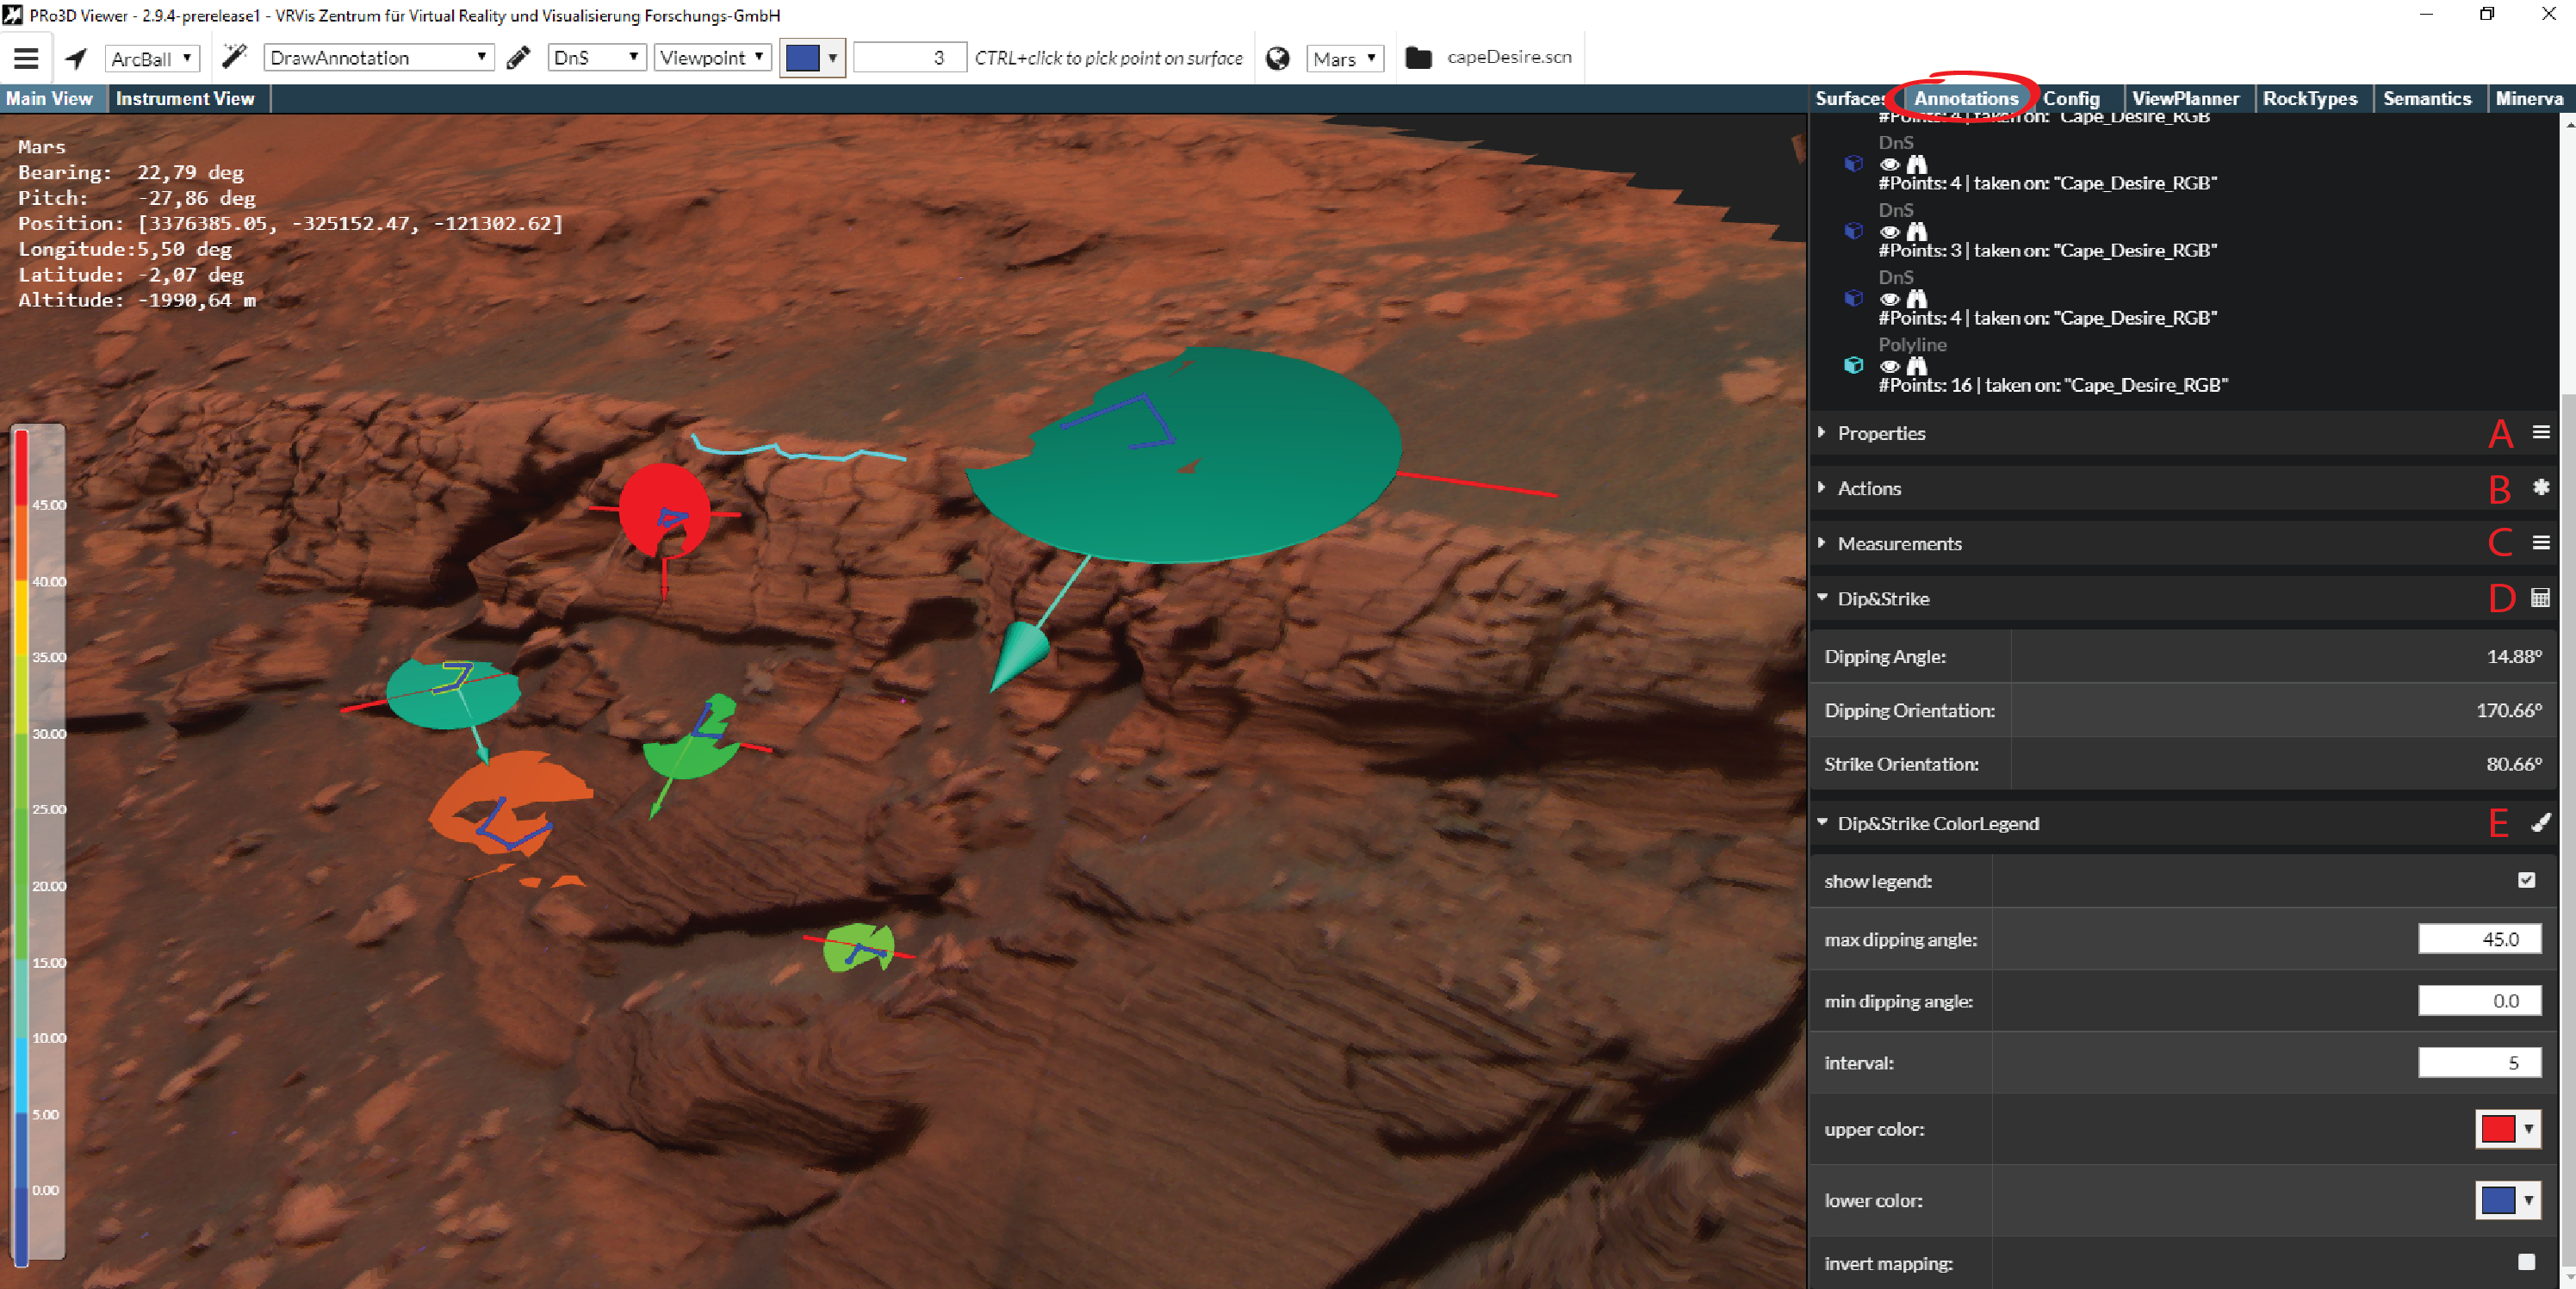
\includegraphics[width=1\textwidth]{pics/DnsAI.png}
    	\caption[Viewer Features DnSColorLegend]{Colorcoding of the Dip\&Strike annotations according to their dipping angles.}
    	\label{fig:dnSColorLegend}
   \end{figure}
	
Measurements for the dip and strike annotations are shown in the Dip\&Strike tab (Figure~\ref{fig:annoProps} D and Figure~\ref{fig:dnSColorLegend} D).\\

The color coding of the DnS annotation's discs and arrows is specified by the dipping angle. The color legend's parameters can be adjusted in the
Dip\&Strike ColorLegend tab shown in Figure~\ref{fig:dnSColorLegend} E.

%----------------------------------------------------------------------------------------Import AnnotationGroups
%\subsubsection{Import Annotations from old viewer versions} 
%
%To import annotations from old scene files click the ``browse'' button in the \textbf{ImportAnnotationGroups} section in the Scene Menu (Figure~\ref{fig:StartMenu}). This opens a folder browser dialog, where you can select an old scene file an click ''Open''.
%The annotations are loaded in the same group hierarchy to the ``root'' group.


%----------------------------------------------------------------------------------------
%	SubSection: ViewPlanner
%----------------------------------------------------------------------------------------
%\subsection{ViewPlanner}
%\label{sec:viewPlanner}

%----------------------------------------------------------------------------------------
%	SubSection: Bookmarks
%----------------------------------------------------------------------------------------
\subsection{Bookmarks}
\label{sec:bookmarks}

%\begin{figure}[h]
    	%\centering
    		%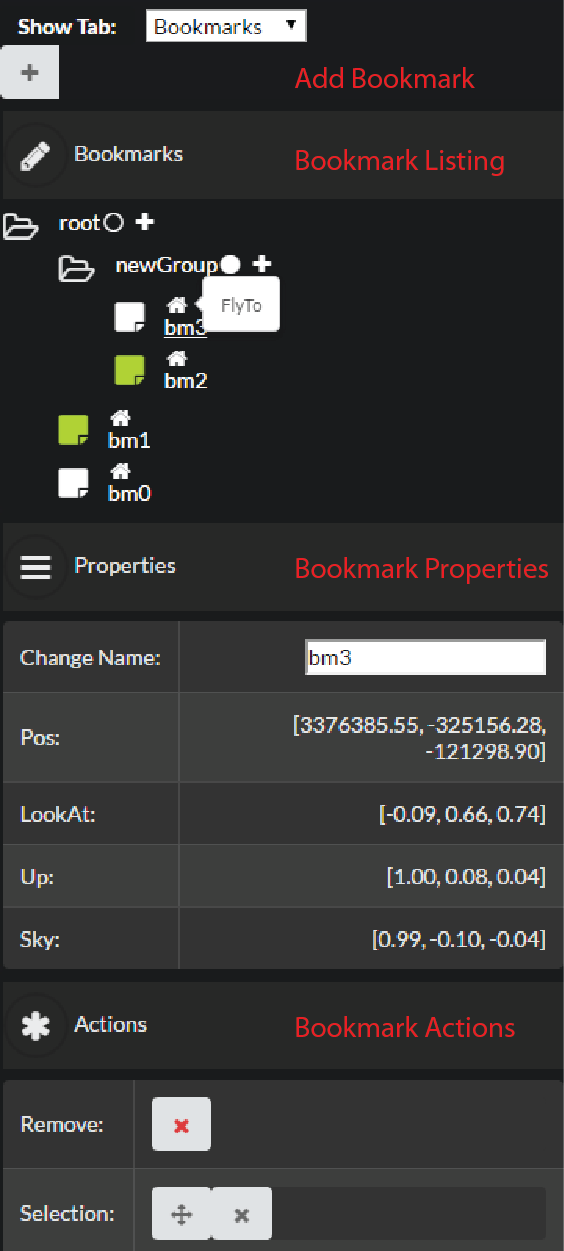
\includegraphics[width=0.5\textwidth]{pics/bookmarks.png}
    	%\caption[Viewer Features Bookmarks]{The bookmarks tab.}
    	%\label{fig:bookmarks}
   %\end{figure}
	
Bookmarks enable the user to record a certain camera viewpoint.
To add a new bookmark click the ``+'' button on top of the page. The new bookmark is added to the active group in the bookmarks listing.
To view the bookmark's properties and actions click on the bookmark's name. Clicking the ``house'' button beside the bookmark's name triggers a FlyTo. For multiselection click on the bookmark's square icons.

%----------------------------------------------------------------------------------------
%	SubSection: Viewer Configuration
%----------------------------------------------------------------------------------------
\subsection{Viewer Configuration}
\label{sec:config}

To edit the viewer properties, select the ``Config'' page.

%----------------------------------------------------------------------------------------Viewer Config
\subsubsection{ViewerConfig} 

A set of major viewer properties can be adjusted:
\begin{itemize}
	\item \textit{Near/Far Plane}: The near- and the far clipping plane are automatically adjusted according to the data to be rendered. The set values are shown in the config panel and can be adjusted afterwards. 
	\item \textit{Navigation Sensitivity}: The navigation sensitivity can also be adjusted by PageUp and PageDown keys. 
	\item \textit{Arrow Length/Thickness}: The arrow length and thickness is set for up- and north vectors, dip and strike vectors and the up- and lookAt vectors in the rover view planner. 
	\item \textit{D+S Plane Size}: The dip and strike measurements plane size, described in Section~\ref{sec:drawAnnotation}
 (Figure~\ref{fig:drawAnnotations}).
	\item \textit{Min/Max Dipping Angle}: The dip and strike measurements dipping angle range. The dipping angle is coded into the color of the disc and arrow of a measurement (Figure~\ref{fig:drawAnnotations}).
	\item \textit{Lod Colors}: The different levels of detail of the surface geometry can be colored in different shades of red.
			This helps to evaluate the export of OPC data.
\end{itemize}

%----------------------------------------------------------------------------------------Coordinate System
\subsubsection{Coordinate System} 

The coordinate system menu shows the position, Up- and North Vector of the coordinate system described in Section~\ref{sec:placeCS}, shown in Figure~\ref{fig:coordinateSystem}.
The Up- and the North Vector are used for the projection measurements (Figure~\ref{fig:drawAnnotations}). Initially the Up Vector's direction is set in the positive z-direction and the North Vector's in the positive y-direction. But you can manipulate the Up Vector manually for different data. Both vectors are computed automatically with picking of a new position for the coordinate system. The north vector is further relevant for bearing measurements. % and the rover placement in the View Planner (see Section 4.6). 

%----------------------------------------------------------------------------------------Camera
\subsubsection{Camera} 

The Camera submenu shows the Location, Forward- and Sky vector of the main camera.
%----------------------------------------------------------------------------------------
%	SubSection: Grouping
%----------------------------------------------------------------------------------------
\subsection{Grouping}
\label{sec:grouping}

%\begin{figure}[h]
    	%\centering
    		%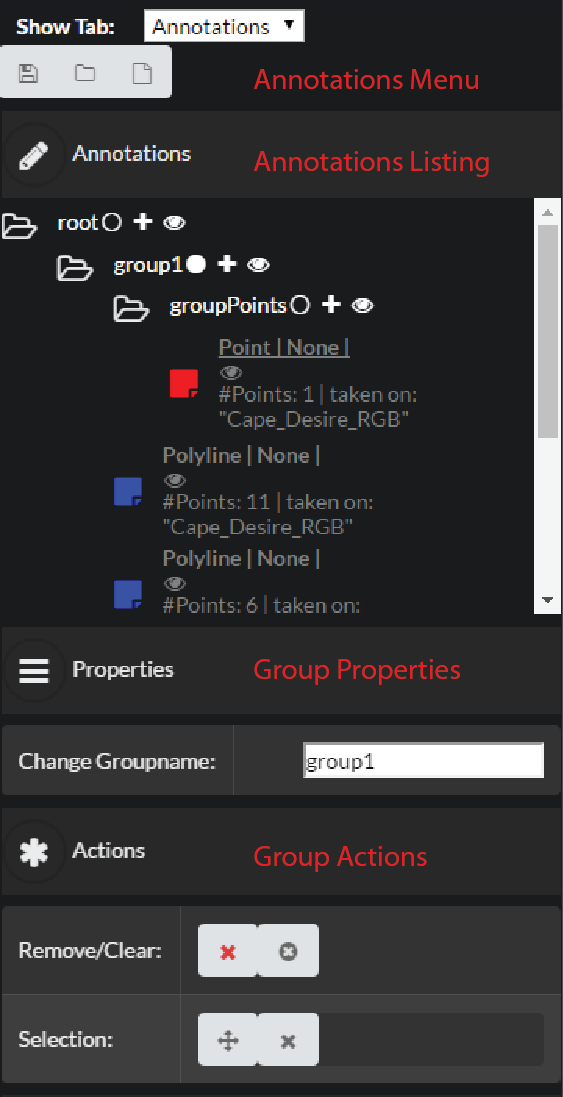
\includegraphics[width=0.5\textwidth]{pics/GroupsProperties.png}
    	%\caption[Viewer Features]{The group properties and actions.}
    	%\label{fig:groupProps}
   %\end{figure}

Grouping is possible for surfaces, annotations and bookmarks.
The ``root'' group is the highest level where you can add leafs and subgroups.
Each group has a context menu:
\begin{itemize}
	\item \textit{Set Active}: The active group gets the new leaf. Per default the ``root'' is active.
	\item \textit{Add Group}: Adds a new and empty subgroup.
	\item \textit{Toggle Group}: Sets all leafs in this group and its subgroups invisible.
\end{itemize}

%----------------------------------------------------------------------------------------Group actions
\subsubsection{Group Actions}
\label{sec:groupActions}

\begin{itemize}
	\item \textit{Remove}: Removes the group with all its leafs and subgroups.
	\item \textit{Clear}: Removes all leafs and subgroups from group but retains the empty group. 
	\item \textit{Selection: Move}: Moves all selected leafs (green squares) to the active group.
	\item \textit{Selection: Clear}: Clears the selection (the leafs were not removed).
\end{itemize}
	
%----------------------------------------------------------------------------------------Leaf actions
\subsubsection{Leaf Actions}
\label{sec:leafActions}

\begin{itemize}
	\item \textit{Remove}: Removes the leaf.
	\item \textit{Selection: Move}: Moves all selected leafs (green squares) to the active group.
	\item \textit{Selection: Clear}: Clears the selection (the leafs were not removed).
\end{itemize}

%----------------------------------------------------------------------------------------
%	SubSection: ViewPlanner
%----------------------------------------------------------------------------------------
\newpage
\subsection{View Planner}
\label{sec:viewplanner}

\begin{figure}[h]
    	\centering
    		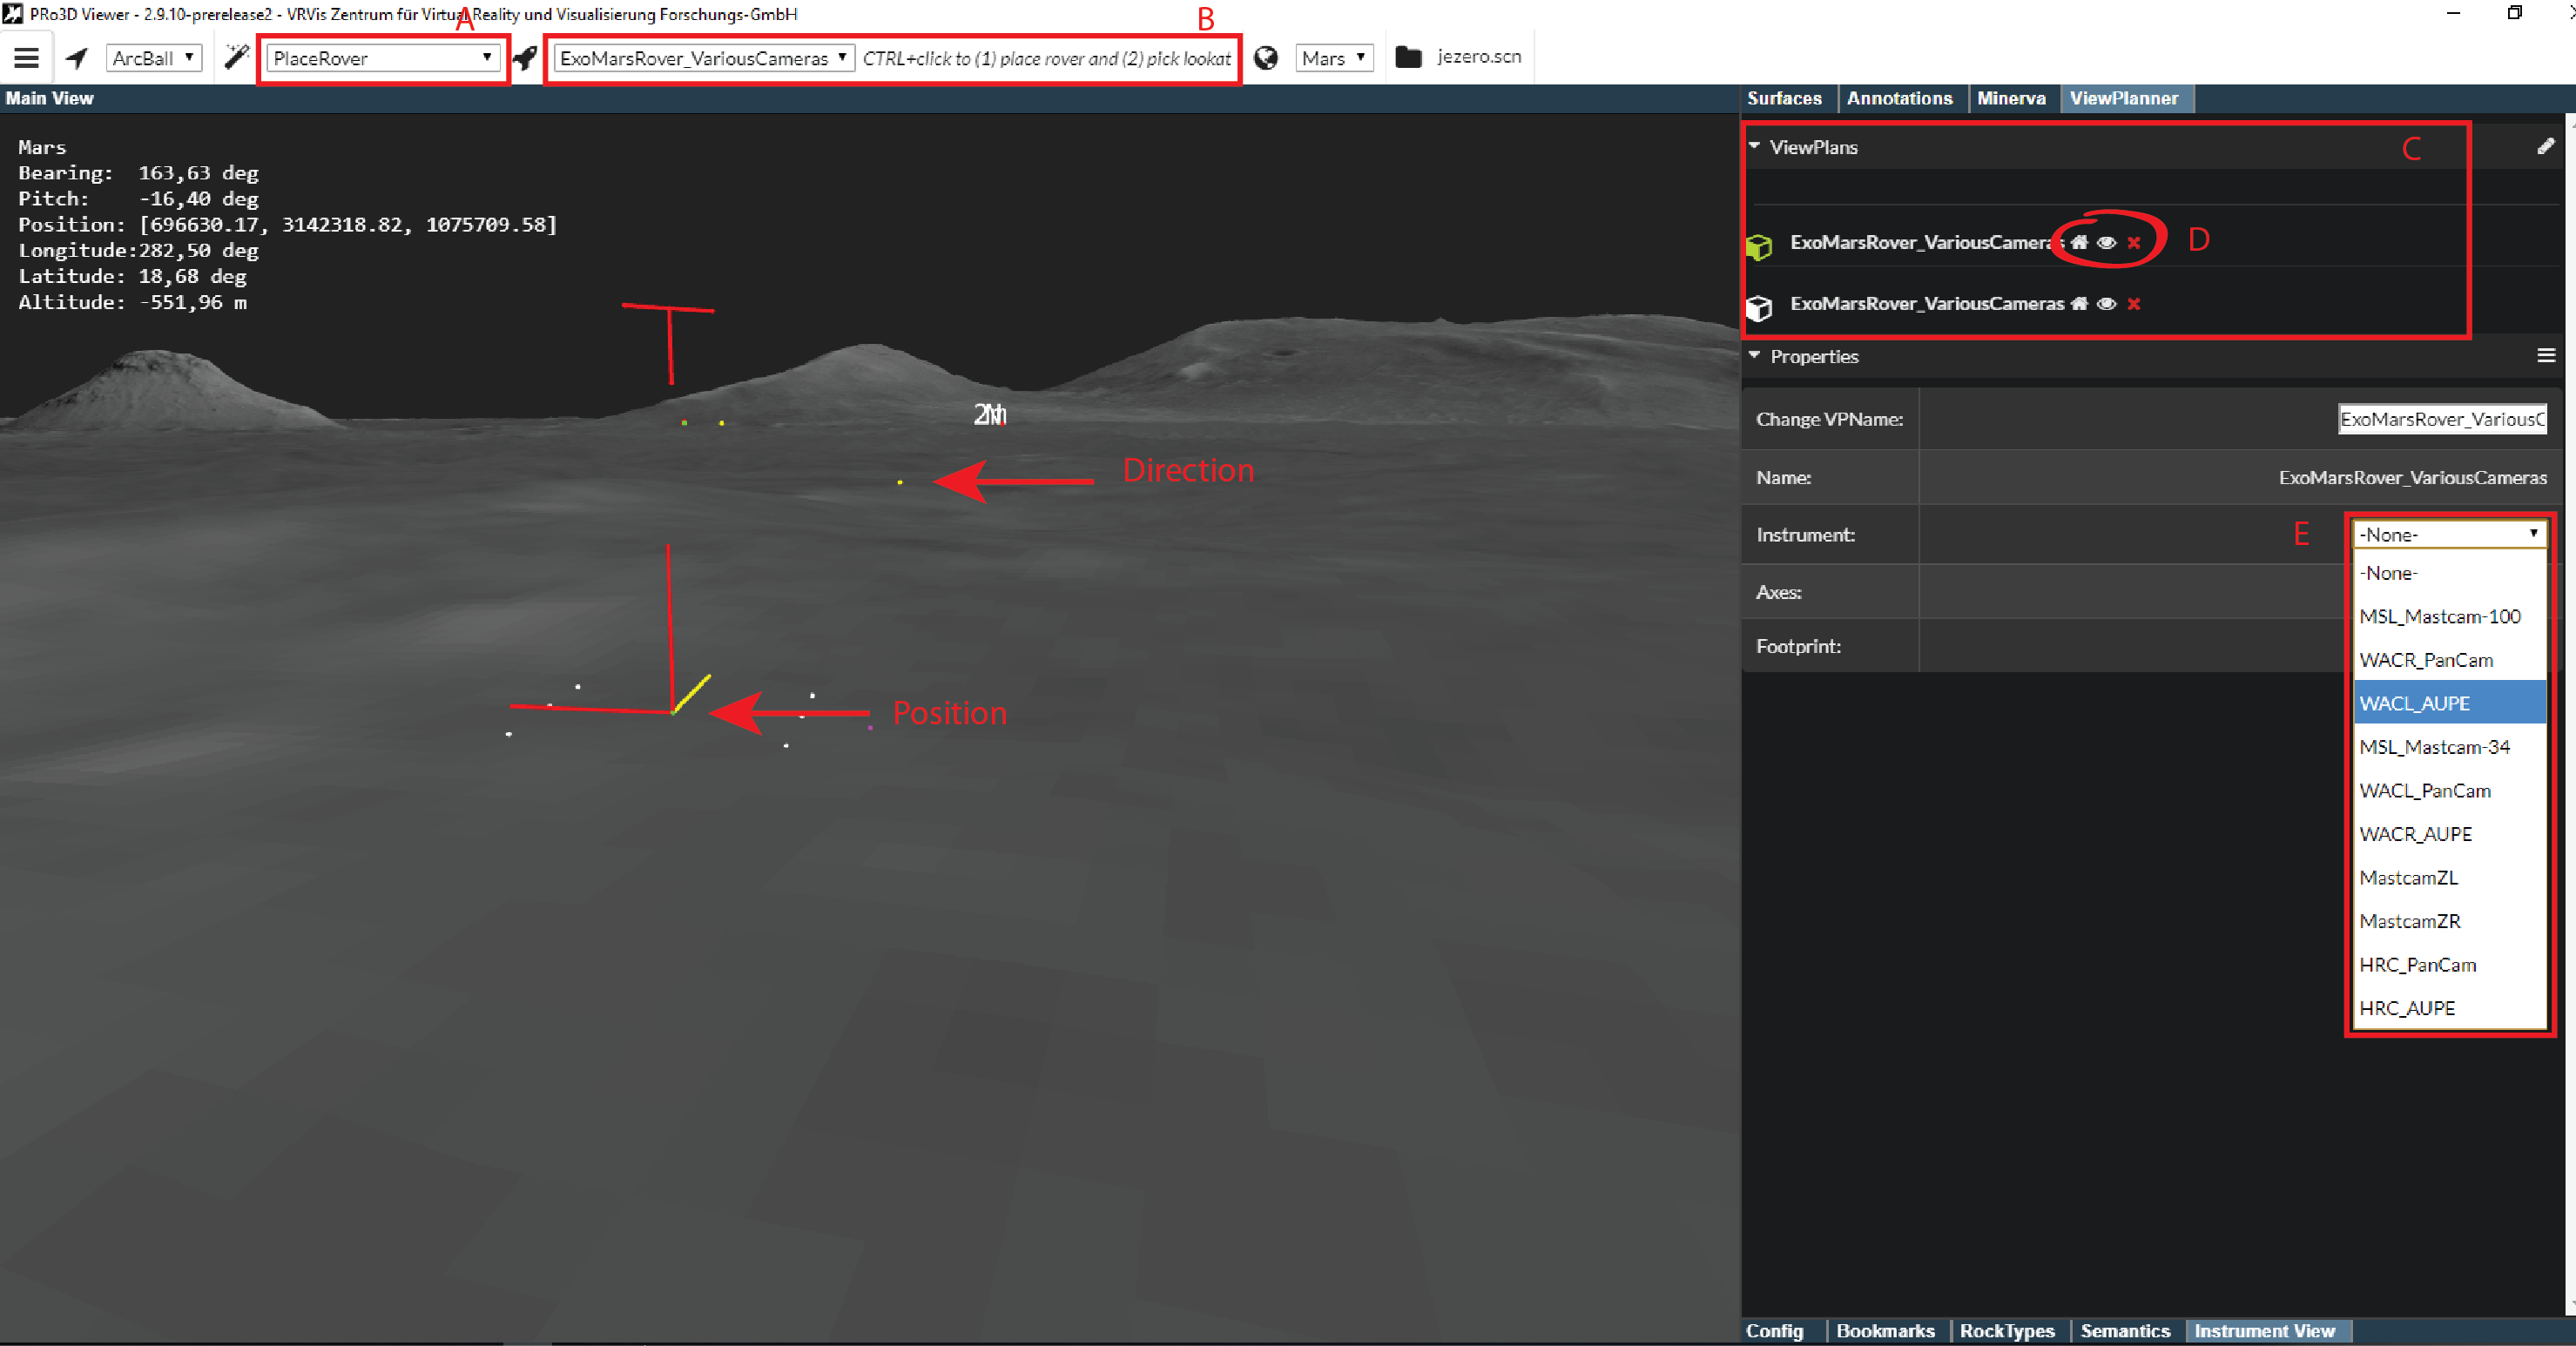
\includegraphics[width=1\textwidth]{pics/ViewPlanner1.png}
    	\caption[View Planner]{The view planner. The rover is placed on the surface in the main view (left). All rovers in the scene are listed in the ViewPlanner tab (right).}
    	\label{fig:viewPlanner}
   \end{figure}
To use the View Planner make sure that a \textbf{rover.xml} file is in the \textbf{\path{Release\InstrumentStuff}} folder. Then you can place one or more rover into your scene.
Therefore set ``PlaceRover'' in the actions menu (Figure~\ref{fig:viewPlanner} A), select a rover model in the rover menu (Figure~\ref{fig:viewPlanner} B), press CTRL+LMB and pick two points on the surface in the main view. The first point (green) is the position and the second point (yellow) the viewing direction of the rover. In the ViewPlanner tab is a listing that shows all ViewPlans in the scene (Figure~\ref{fig:viewPlanner} C). There is a little menu beside each ViewPlan shown in Figure~\ref{fig:viewPlanner} D:
\begin{itemize}
	\item FlyTo: clicking on the ``house button'' triggers an animation to the camera position from where the rover placement happened.
	\item (In)Visible: switch the rover to visible\textbackslash invisible.
	\item Remove: clicking on the red ``x'' removes the View Plan from the list and the view.
\end{itemize}
Select a view plan by clicking on the square icon in front of it to adjust it's properties:
\begin{itemize}
	\item ChangeVPName: change the name and press the enter button.
	\item Name: shows the rover's name.
	\item Instrument: select an instrument (camera) from the list (Figure~\ref{fig:viewPlanner} E).
\end{itemize}
\begin{figure}[h]
    	\centering
    		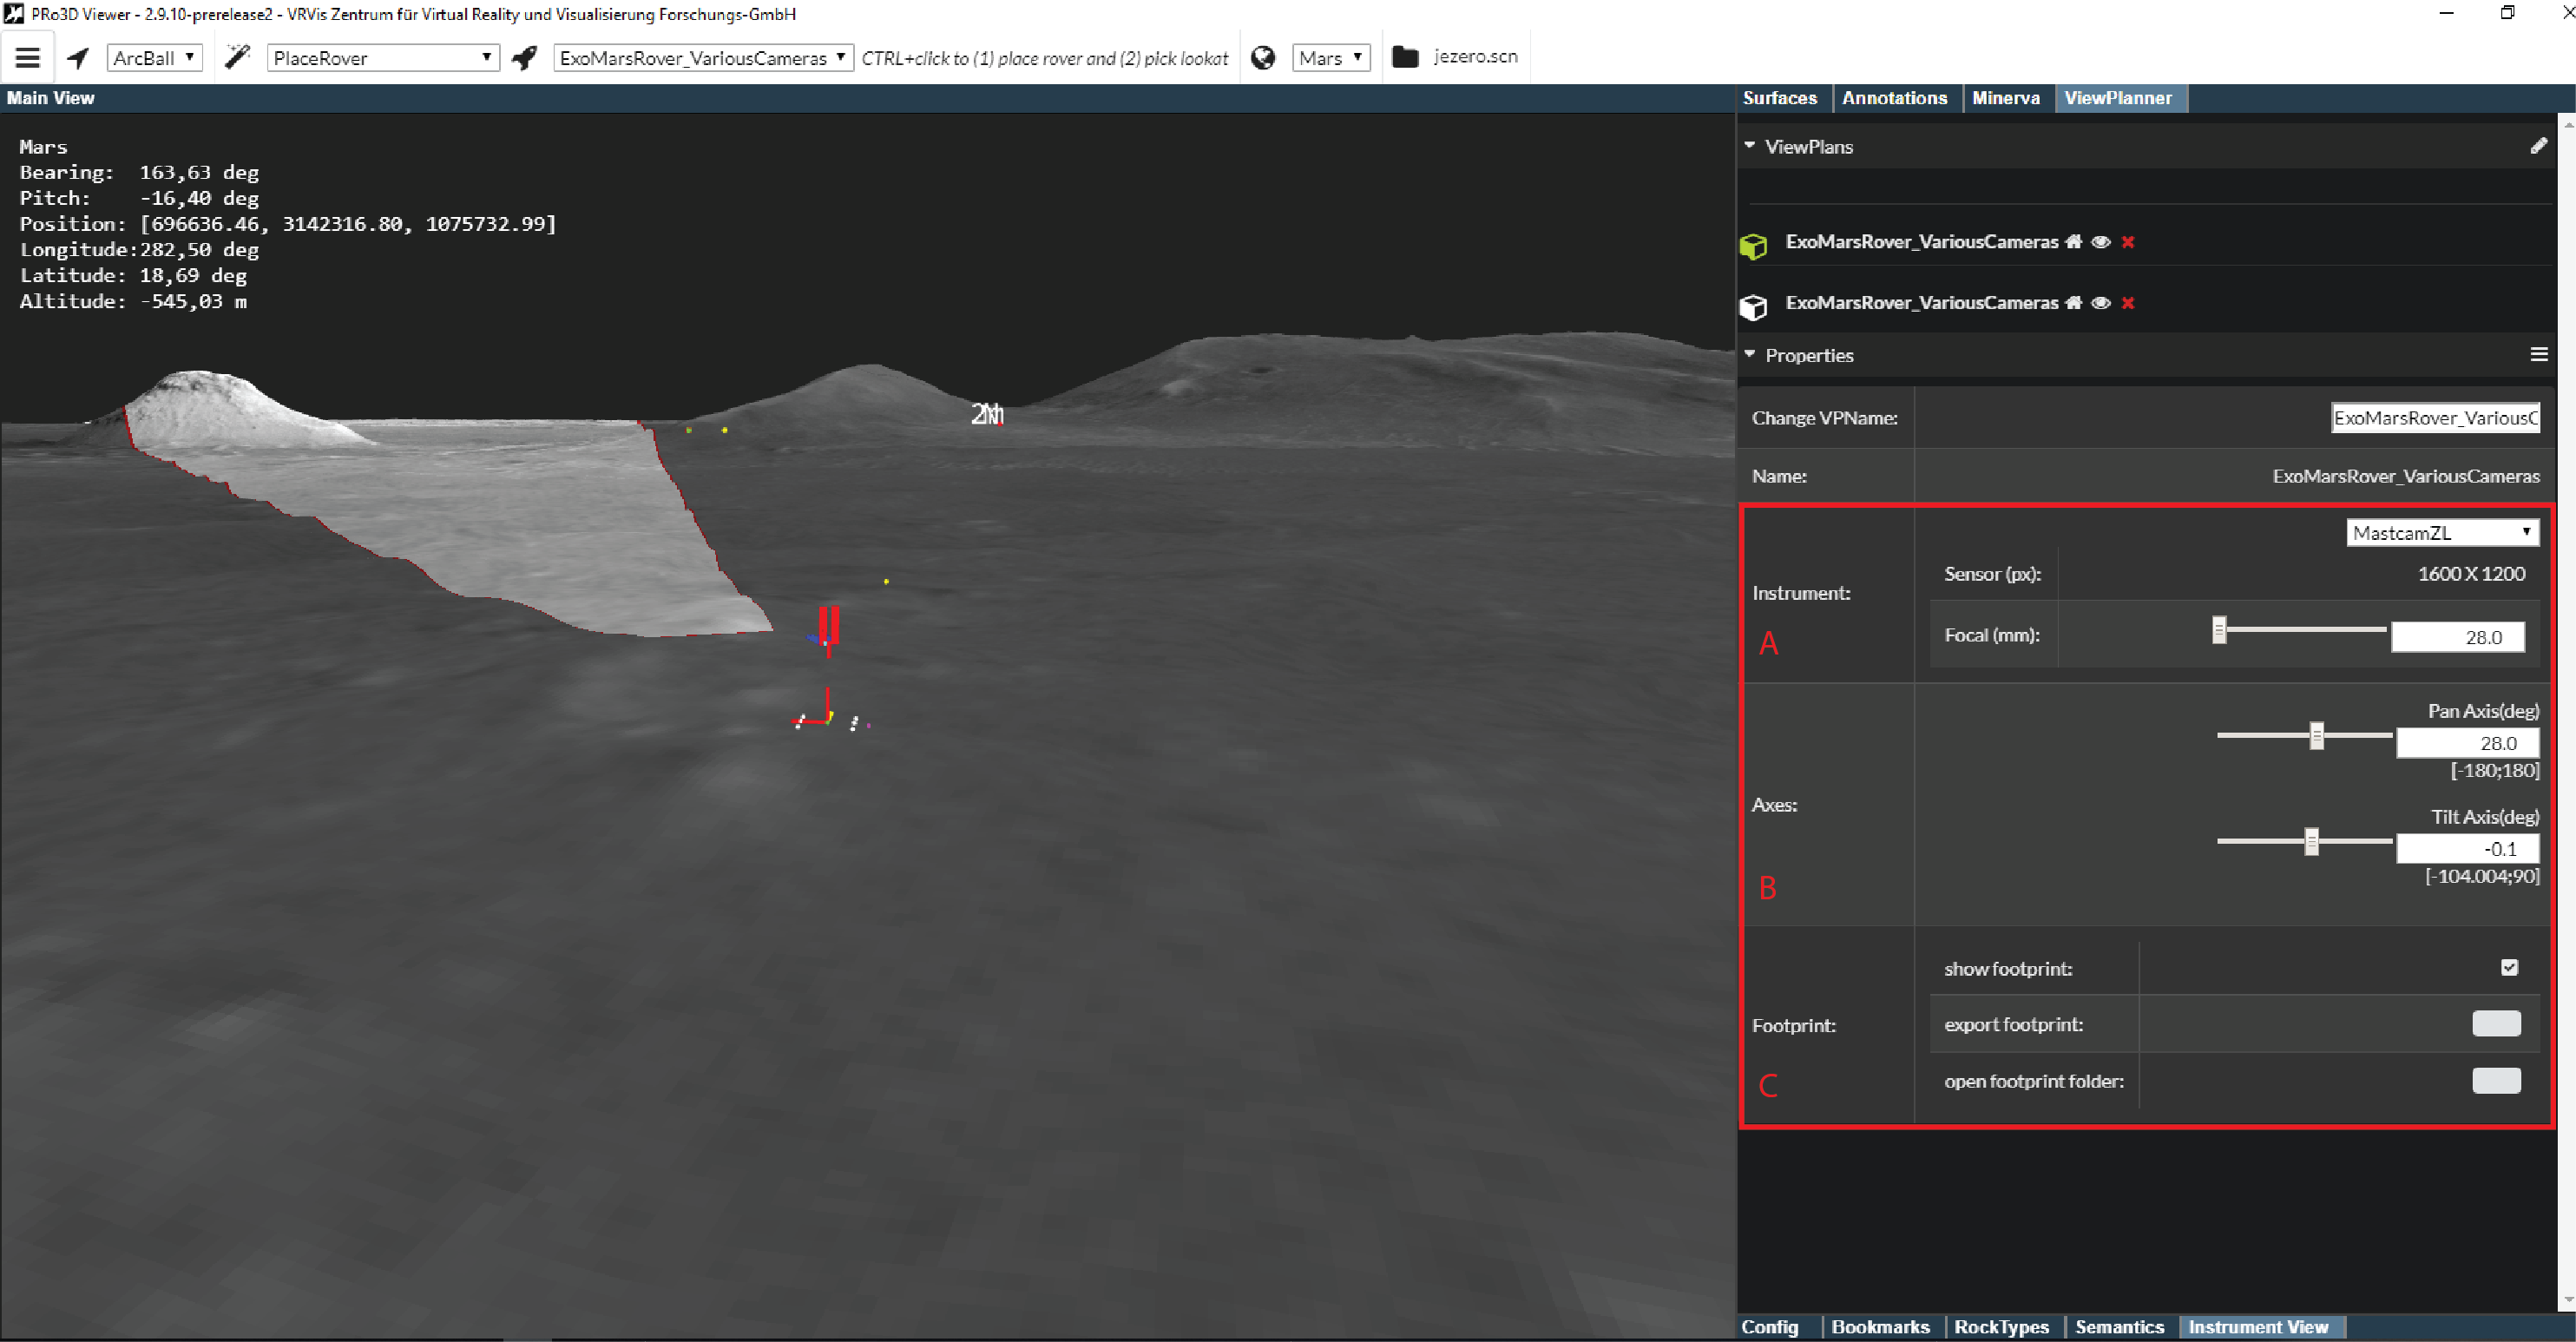
\includegraphics[width=1\textwidth]{pics/ViewPlannerGuiAi.png}
    	\caption[View PlannerGui]{The footprint for the selected camera is shown in light gray on the surface in the main view. In the properties panel (right) you can adjust the rover and camera parameters.}
    	\label{fig:viewPlannerGui}
   \end{figure}
When a camera is selected you can change the instrument parameters as shown in Figure~\ref{fig:viewPlannerGui} A:
\begin{itemize}
	\item Sensor (px): the image size in pixel.
	\item Focal (mm): the focal length of the camera sensor (zoom).
\end{itemize}
You can also change the rover's pan- and tilt axis (in degree) (Figure~\ref{fig:viewPlannerGui} B).
In the main view the footprint of the selected camera is shown in light gray. For the footprint there are following settings:
\begin{itemize}
	\item show footprint: you can enable\textbackslash disable the footprint in the main view.
	\item export footprint: you get one screenshot from the main view, one from the instrument view (Figure~\ref{fig:instView}) and a \textbf{*.svx} file with diverse meta information.
	\item open footprint folder: opens the folder with the screenshots and the meta file.
\end{itemize}
\begin{figure}[h]
    	\centering
    		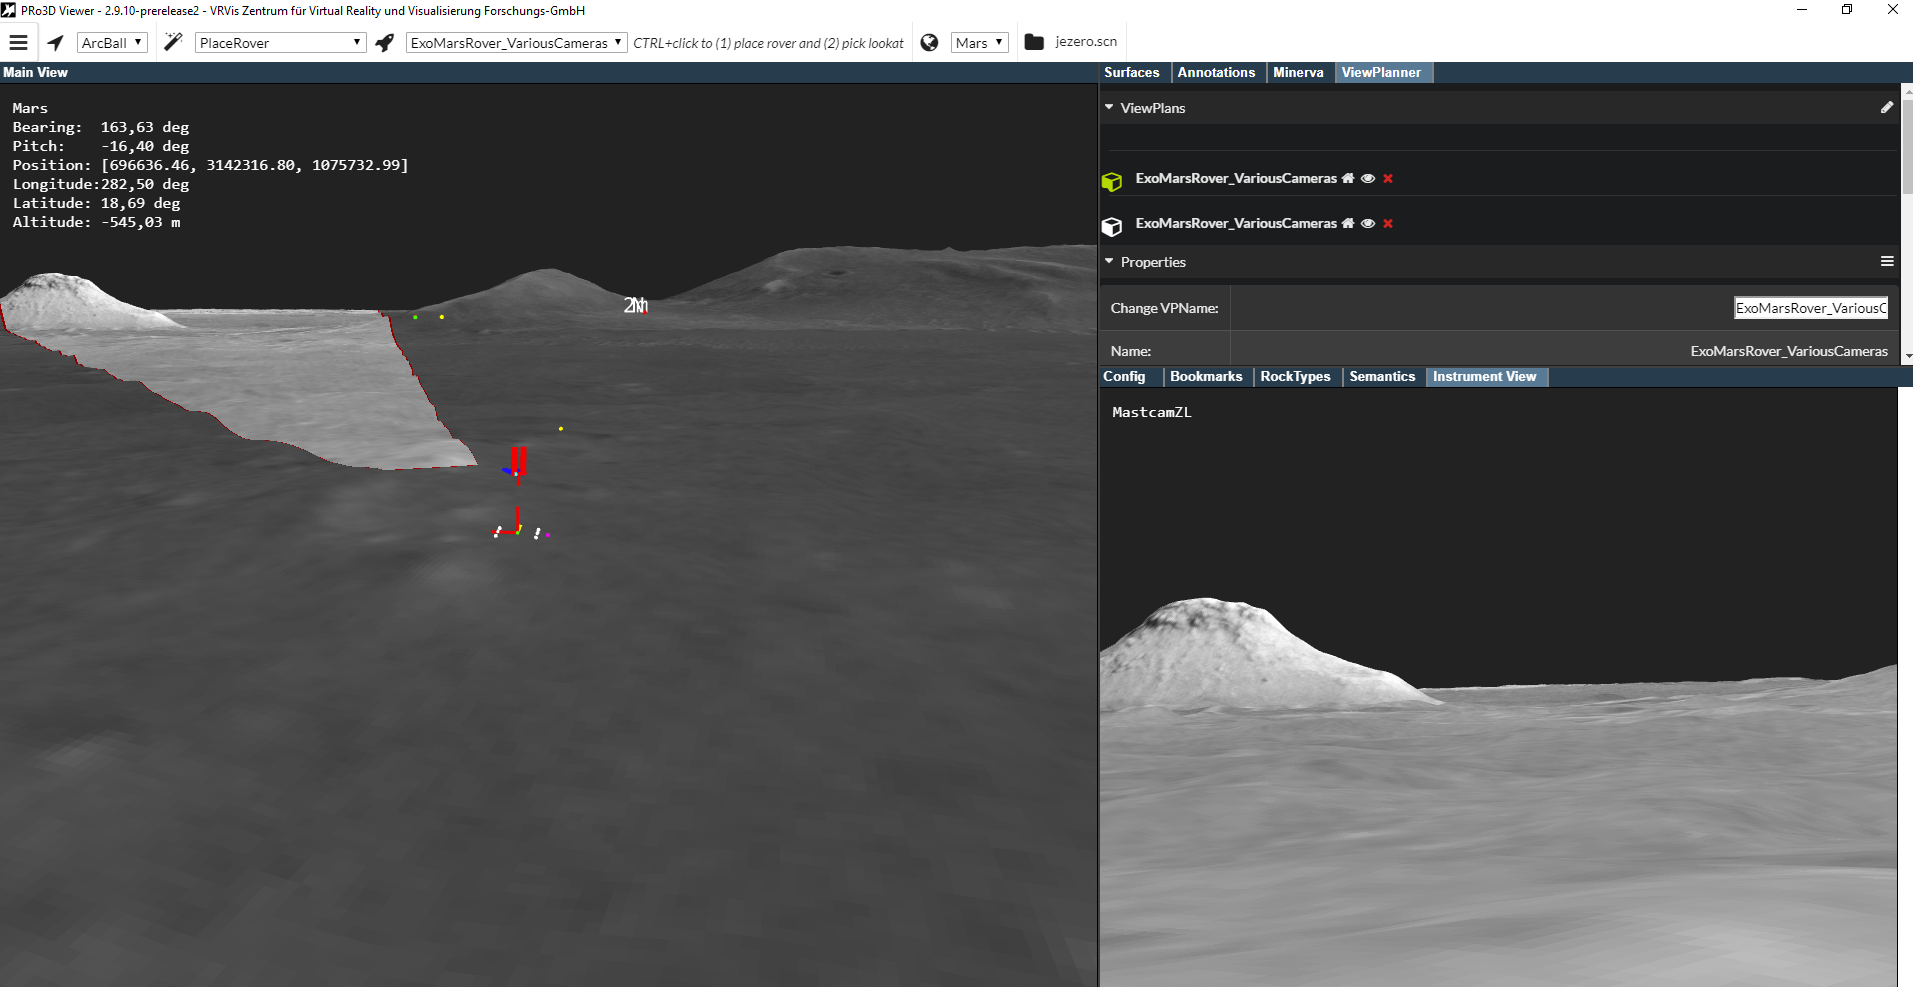
\includegraphics[width=1\textwidth]{pics/InstrumentView.png}
    	\caption[Instrument View]{The instrument view (right) shows the instrument's camera view.}
    	\label{fig:instView}
   \end{figure}
%----------------------------------------------------------------------------------------
%	Section: Minerva
%----------------------------------------------------------------------------------------
%----------------------------------------------------------------------------------------
%	Section: Minerva
%----------------------------------------------------------------------------------------
\section{Minerva}

\begin{figure}[h]
    	\centering
    		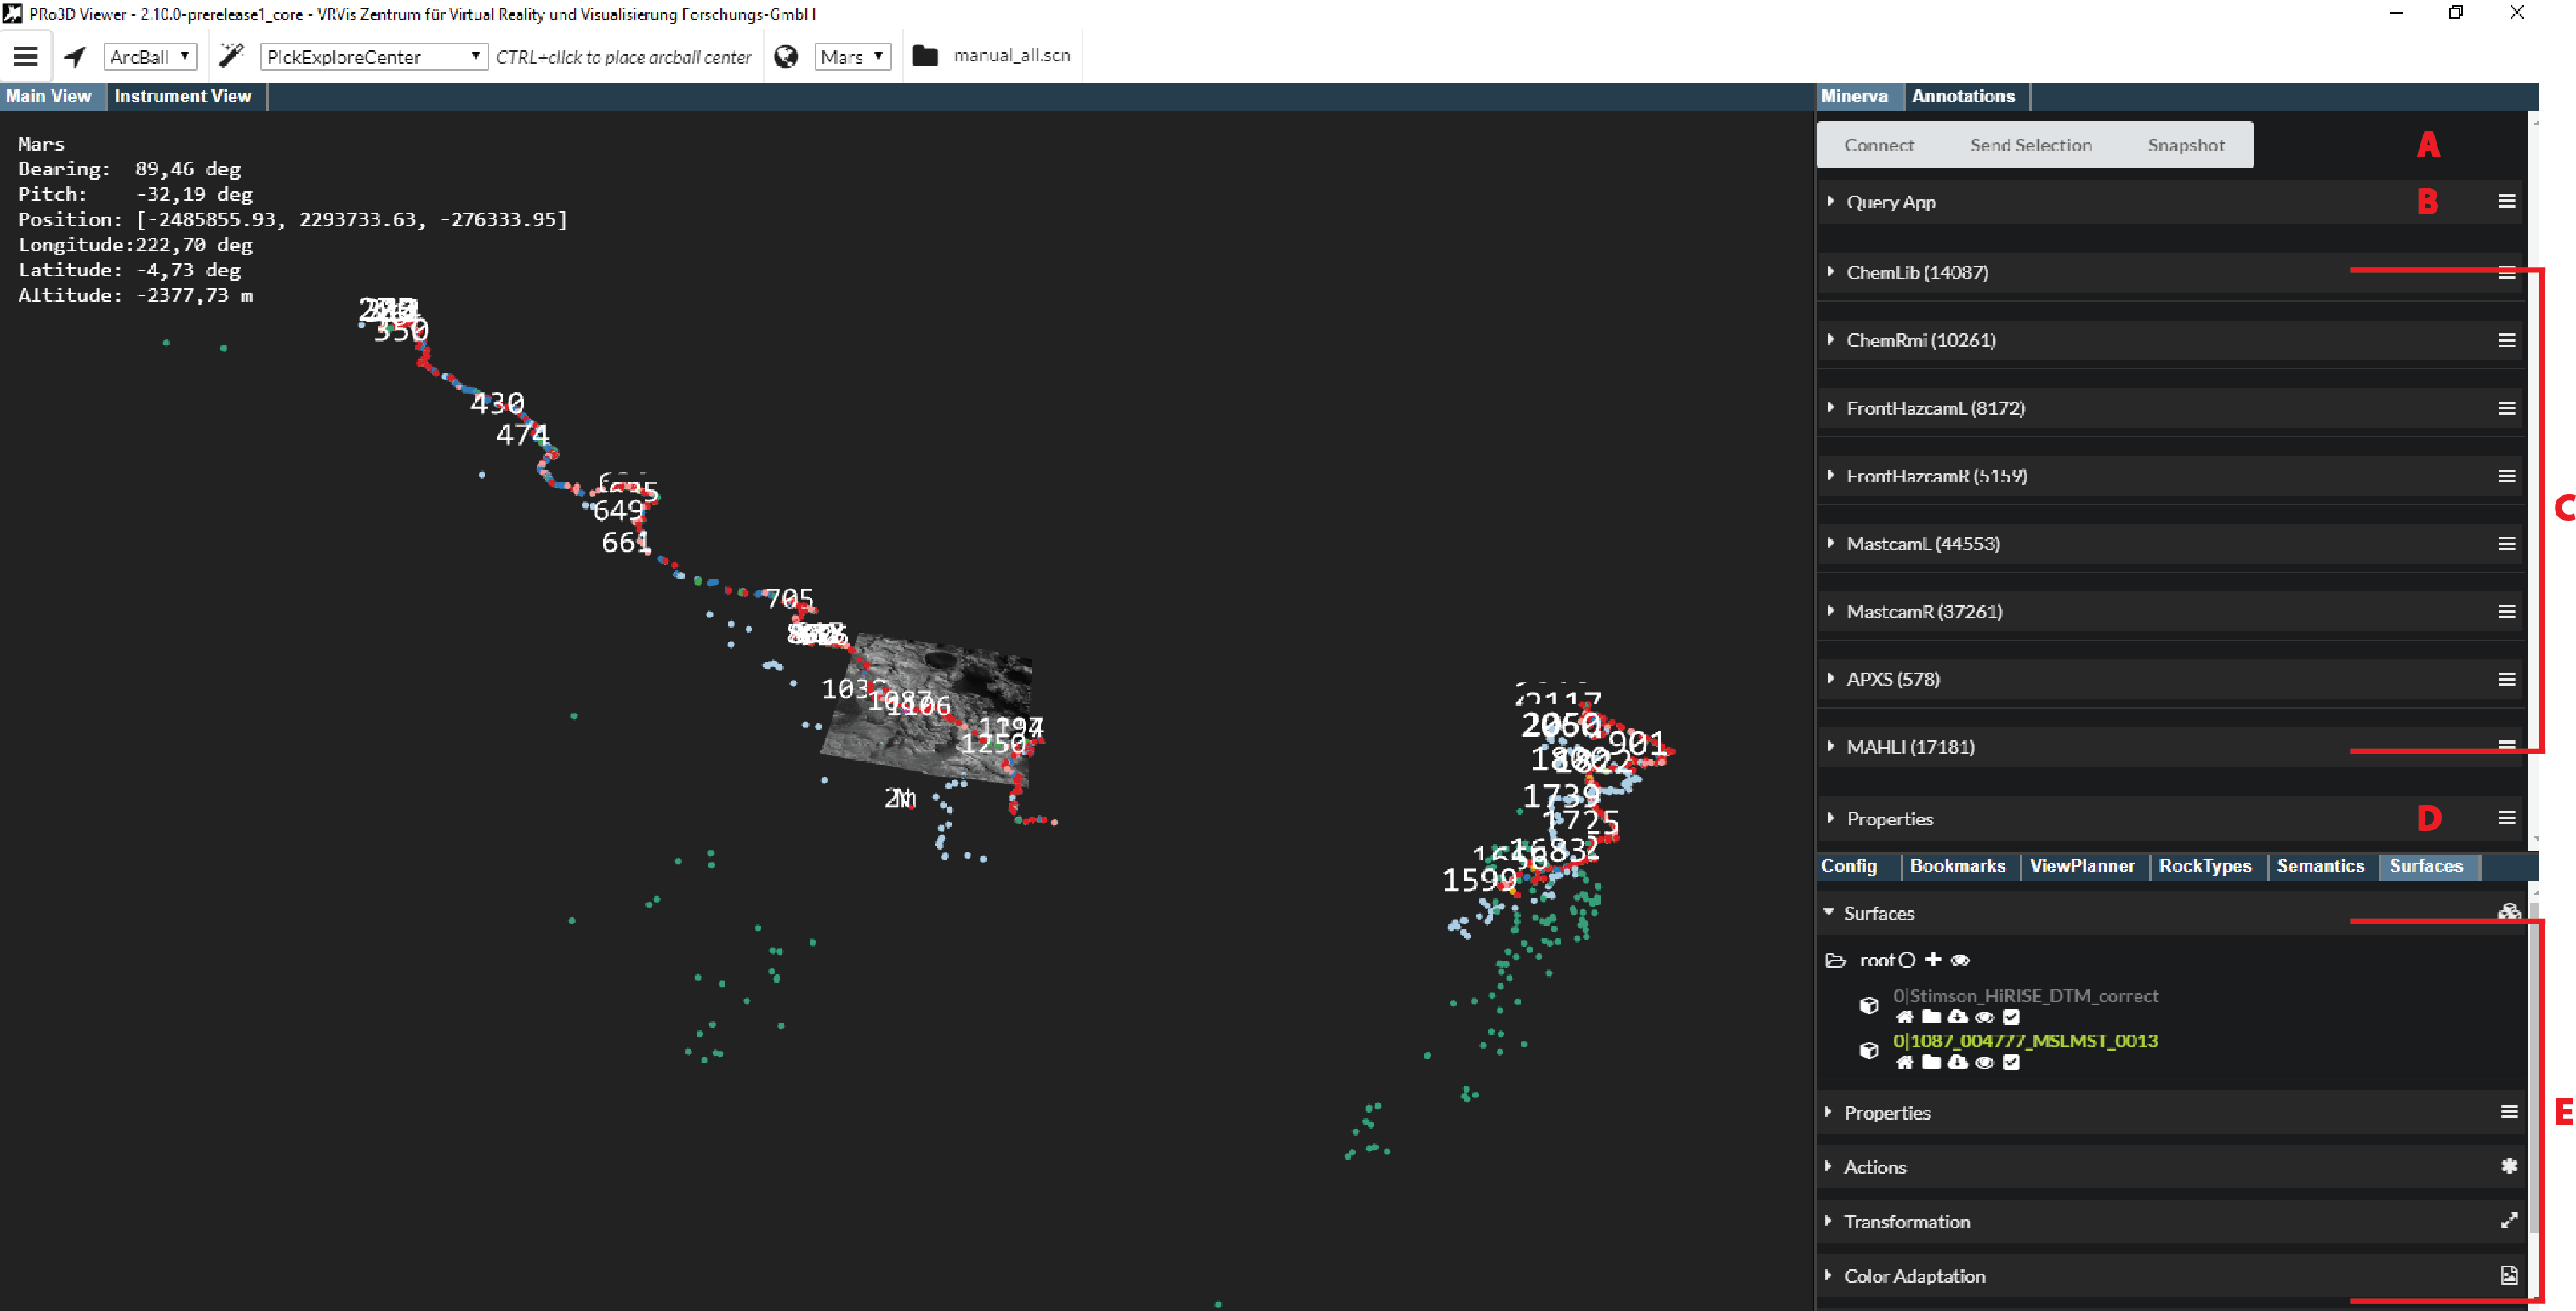
\includegraphics[width=1\textwidth]{pics/MinervaAI.png}
    	\caption[Start Minerva]{The Minerva Application. The Main View (left) shows the surface data with the products. There are different interaction possibilities for the products in the Minerva tab (right). A: Visplore communication, B: Query App to reduce the shown products by the mean of different criteria, C: Product listing, D: Properties of the last selected product, E: Surface tab.  }
    	\label{fig:StartMinerva}
   \end{figure}

%----------------------------------------------------------------------------------------
%	SubSection: Start Minerva
%----------------------------------------------------------------------------------------
\subsection{Start Minerva}
\label{sec:startMinerva}

Before you start the Minerva Application make sure that the \textbf{dump.csv} file is in the \textbf{\path{Release\netcoreapp2.0\MinervaData}} folder.
Then start the viewer by clicking the PRo3D.exe as described in Section~\ref{sec:startViewer}. The Minerva data from the dump.csv file is loaded and the products are listed in the ``Minerva'' tab as shown in Figure~\ref{fig:StartMinerva} C.  Load the surface data as described in Section~\ref{sec:addSurface}.
How to explore and adjust the surfaces is described in Section~\ref{sec:surfaces}.
You can save the scene as described in Section~\ref{sec:addSurface}.

%----------------------------------------------------------------------------------------
%	SubSection: Minerva Features
%----------------------------------------------------------------------------------------
\subsection{Minerva Features}
\label{sec:minervaFatures}

%----------------------------------------------------------------------------------------Visplore
\subsubsection{Visplore}

Visplore is a powerful visual analytics tool that allows the handling of huge and heterogeneous data and provides different perspectives onto the data that help finding causalities and allow an easy examination of the data's plausibility. 
For this project an interface was implemented that allows an interconnected workflow between PRo3D and Visplore.
To communicate with Visplore use the tree buttons shown in Figure~\ref{fig:StartMinerva} A:
\begin{itemize}
	\item \textbf{Connect:} Connect to Visplore.
	\item \textbf{Send Selection:} Send the selected products to Visplore.
	\item \textbf{Snapshot:} Send a snapshot of the MainView to the Visplore MapView.
\end{itemize}
For more information how to use Visplore for Minerva, please refer to the Visplore manual.

%----------------------------------------------------------------------------------------Query App
\subsubsection{QueryApp}
	
	\begin{figure}[h]
    	\centering
    		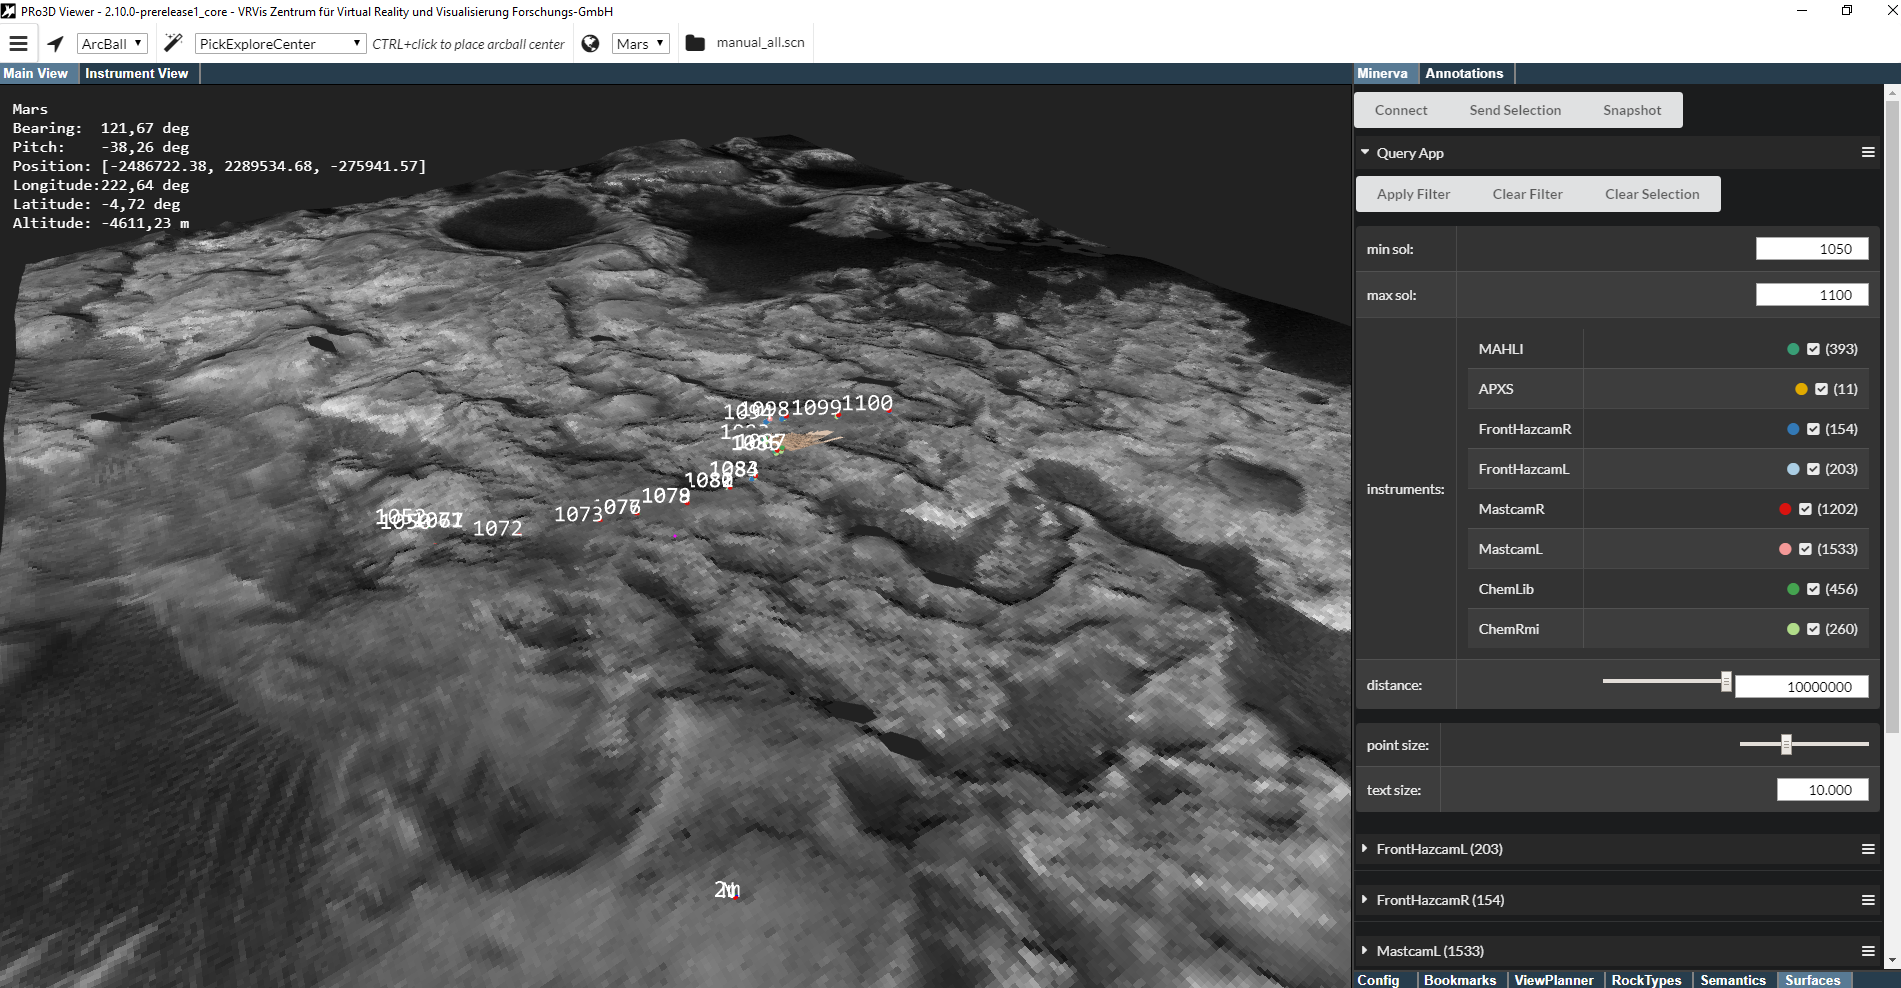
\includegraphics[width=1\textwidth]{pics/QueryApp.png}
    	\caption[Query App]{The Query App (right).}
    	\label{fig:QueryApp}
   \end{figure}

The Query App provides the possibility to cut down the number of shown products by the mean of different criteria. These criteria are:
\begin{itemize}
	\item \textbf{min- and max sol:} All products with sol numbers in the given range are shown.
	\item \textbf{instruments:} Only the products with checked instruments are shown.
	\item \textbf{distance:} The distance between the camera location and the shown products is less than the entered distance value.
\end{itemize}
You can use one ore more criteria and press the \textbf{``ApplyFilter''} button in top of the Query App menu. Now only the filtered products are shown. Change the queries and click ``ApplyFilter'' again to change the shown products. To get all products click the \textbf{``ClearFilter''} button. 
You can also change the \textbf{point size} of the rendered products in the Main View, and the \textbf{text size} of the shown sol numbers.

%----------------------------------------------------------------------------------------Product Listing
\subsubsection{Product Listing and Selection}
\label{sec:selection}

\begin{figure}[h]
				\centering
					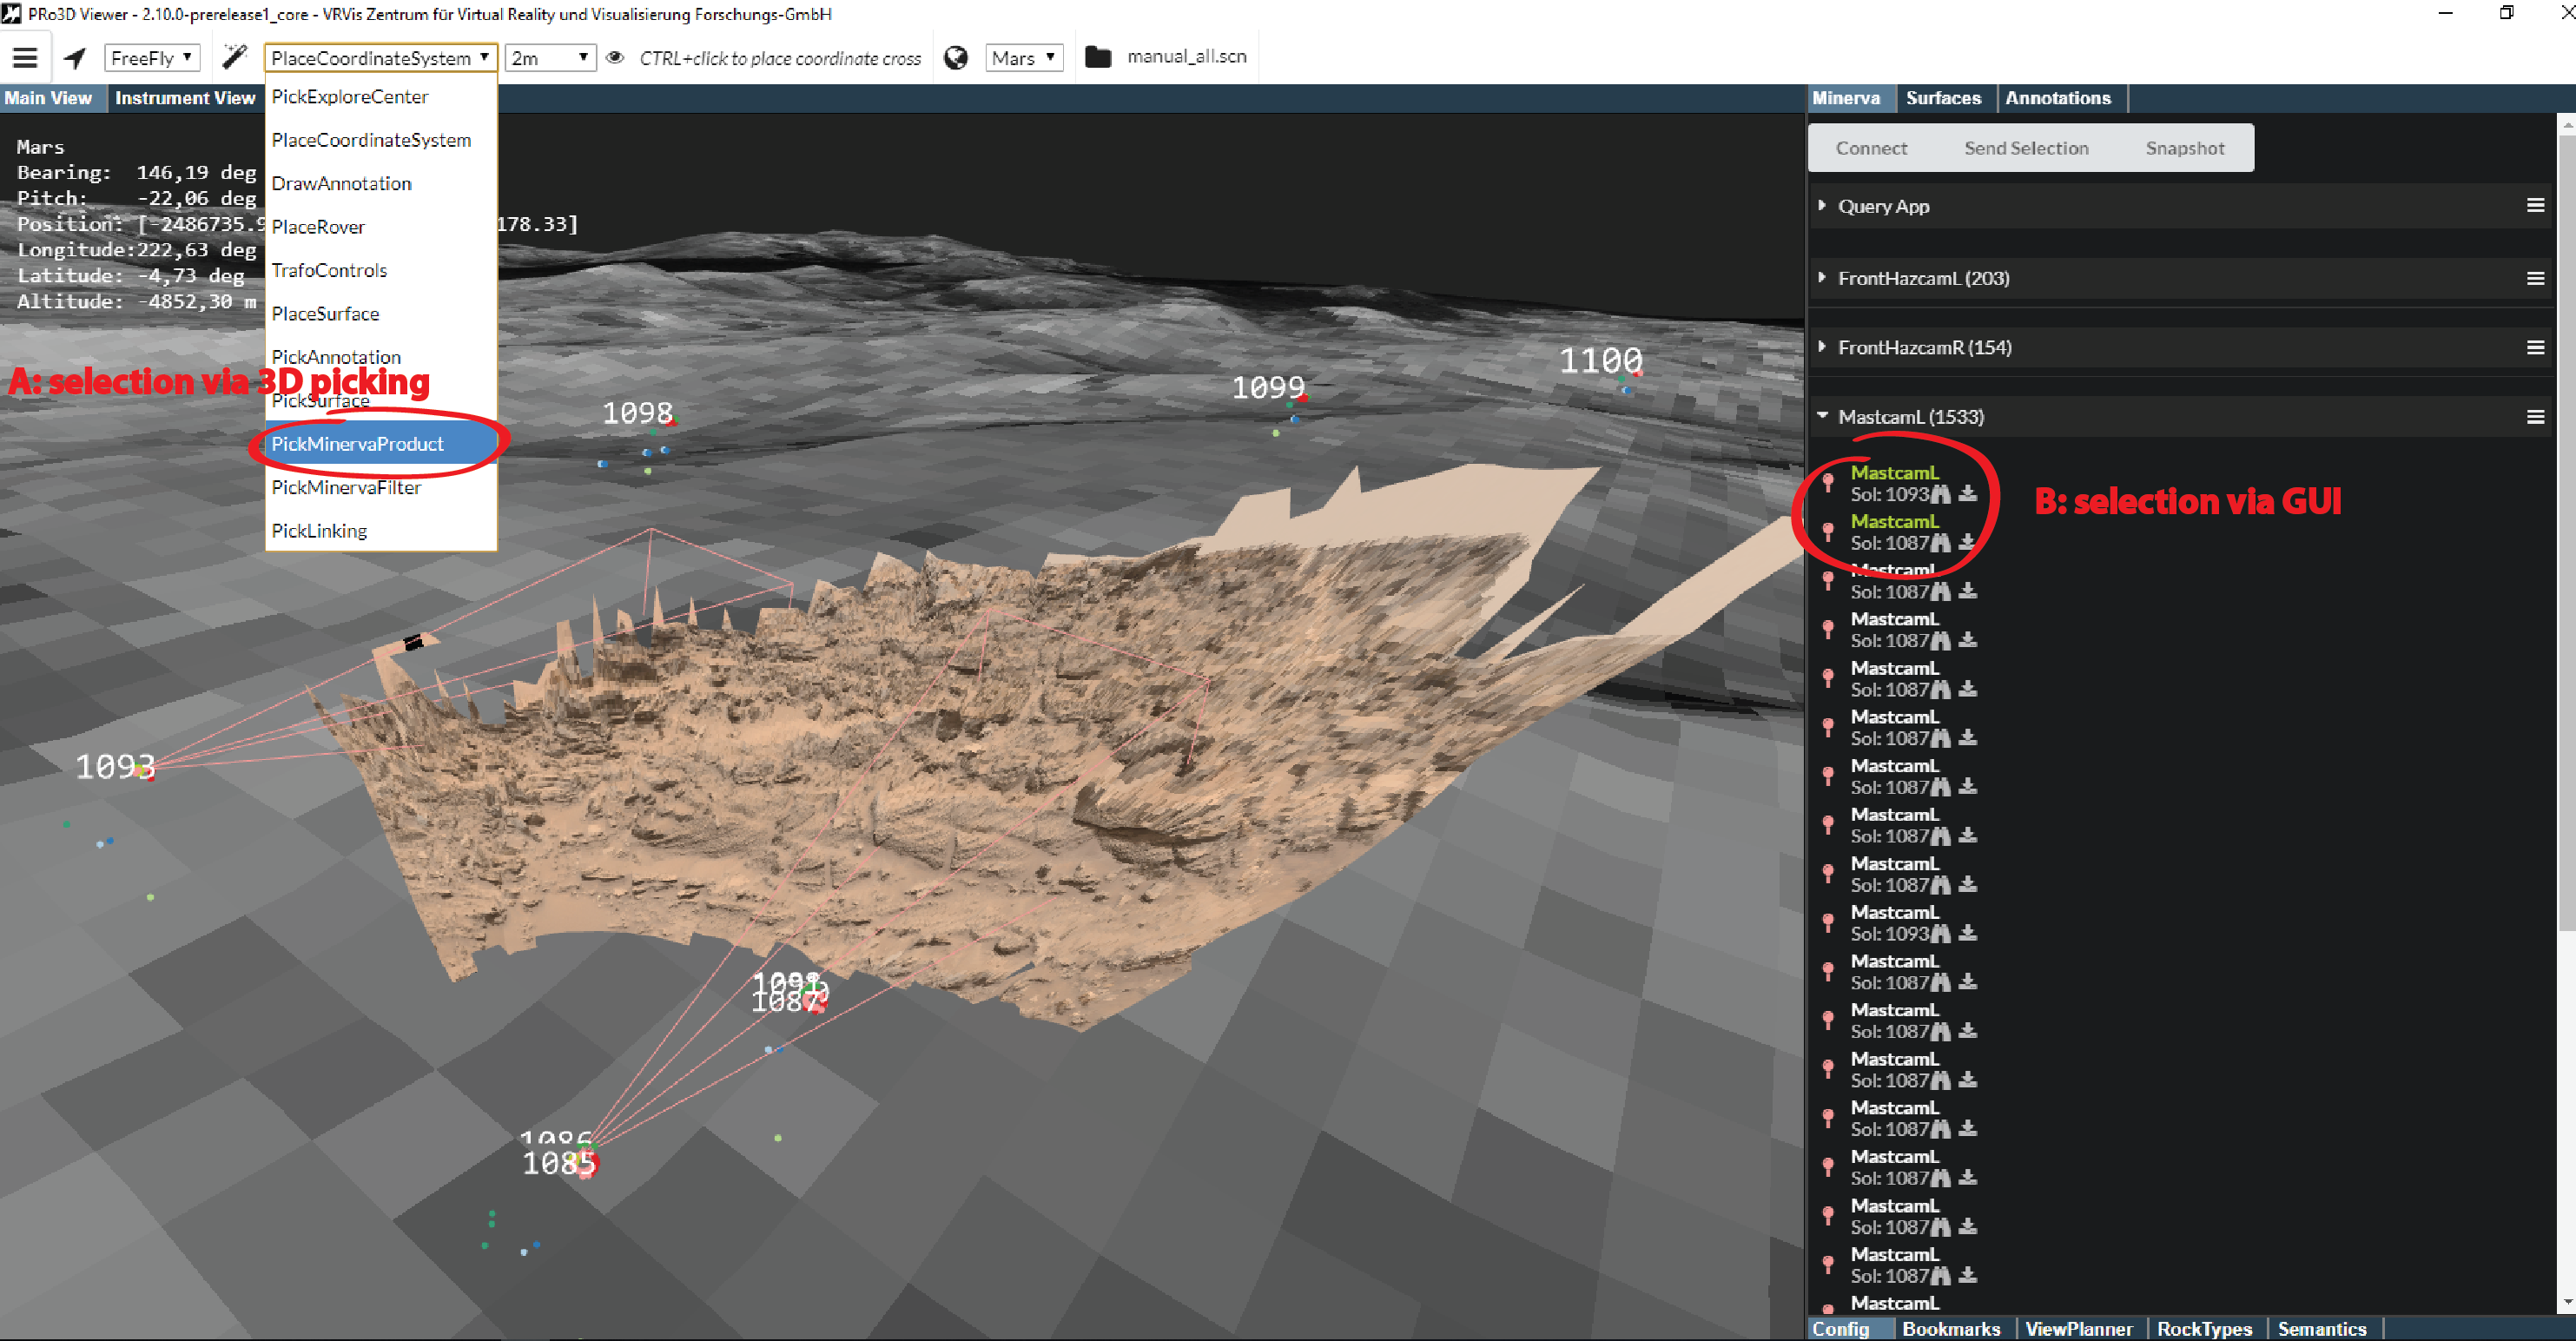
\includegraphics[width=1\textwidth]{pics/ListingAI.png}
				\caption[Product Listing]{The products are grouped by instruments. A product can either be selected in the listing (B) or in the Main View (A). }
				\label{fig:ProductListing}
		 \end{figure}
		
The products are grouped in the gui by their instruments (Figure~\ref{fig:StartMinerva} C) where the first 20 products for each instrument are listed.
You can select single products by clicking on the products's name, which turns its color to green. Or you can set ``PickMinervaProduct'' in the actions menu (Figure~\ref{fig:ProductListing}), press CTRL+LMB and pick the product in the main view. Then you can see the product's properties in the properties panel, described in the next Section~\ref{sec:productProps}. 

\begin{figure}[h]
				\centering
					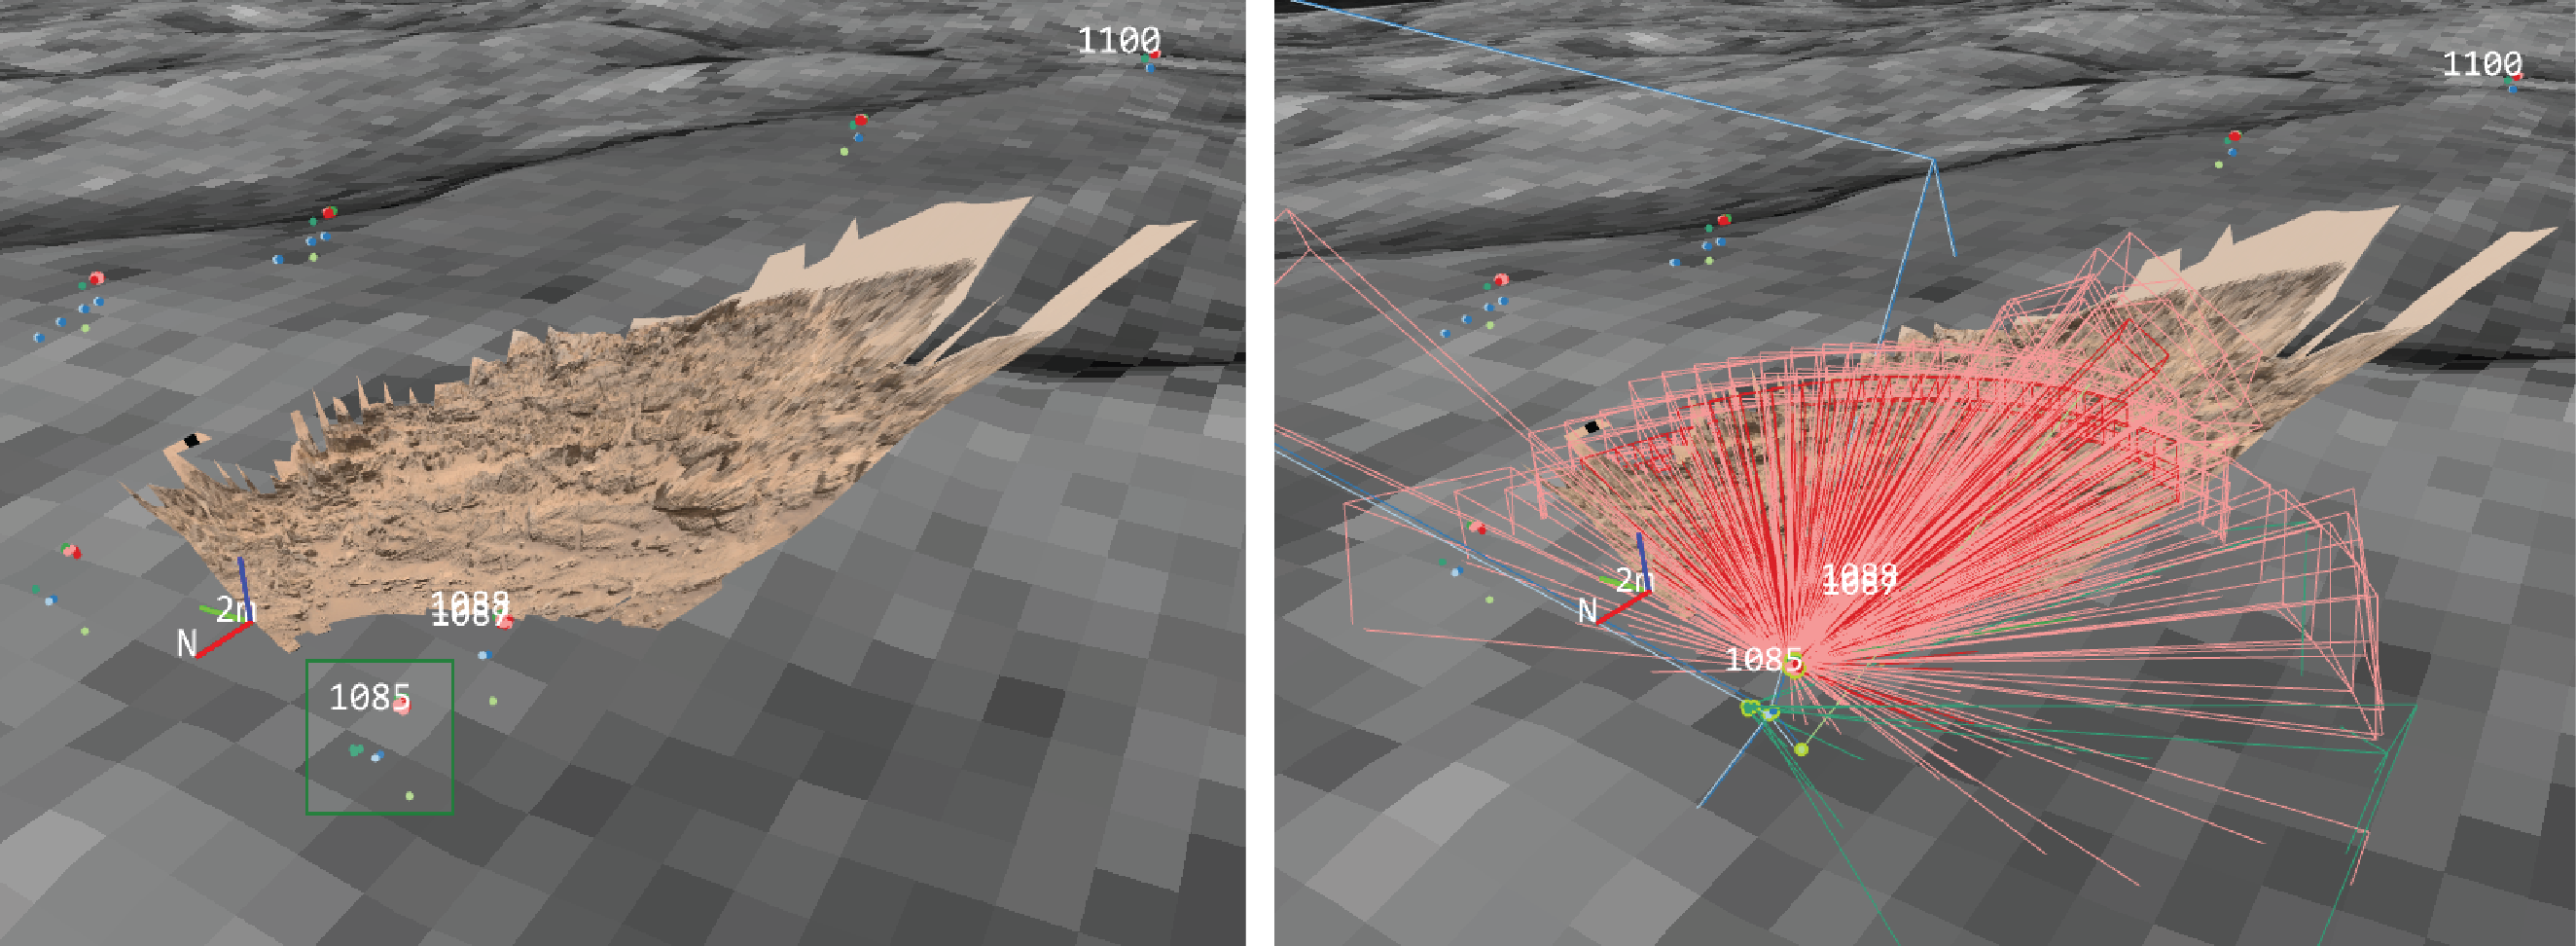
\includegraphics[width=1\textwidth]{pics/MultiSelAI.png}
				\caption[Multi Selection]{A rectangle is spanned over multiple products (left). All products selected by the rectangle (right).}
				\label{fig:MultiSel}
		 \end{figure}
		
It is also possible to select multiple products. Press SHIFT+LMB and drag a rectangle (Figure~\ref{fig:MultiSel} left). When you release the LMB, all products in this area are selected (Figure~\ref{fig:MultiSel} right). \\
Under the products's name is a little menu:
\begin{itemize}
  \item \textbf{The Sol Number}
	\item \textbf{FlyTo}: A click on the button triggers a FlyTo animation.
	\item \textbf{GetTif}: Downloads the product's tif image.
\end{itemize}

	
	
%----------------------------------------------------------------------------------------Product Properties
\subsubsection{Product Properties}
\label{sec:productProps}

\begin{figure}[h]
				\centering
					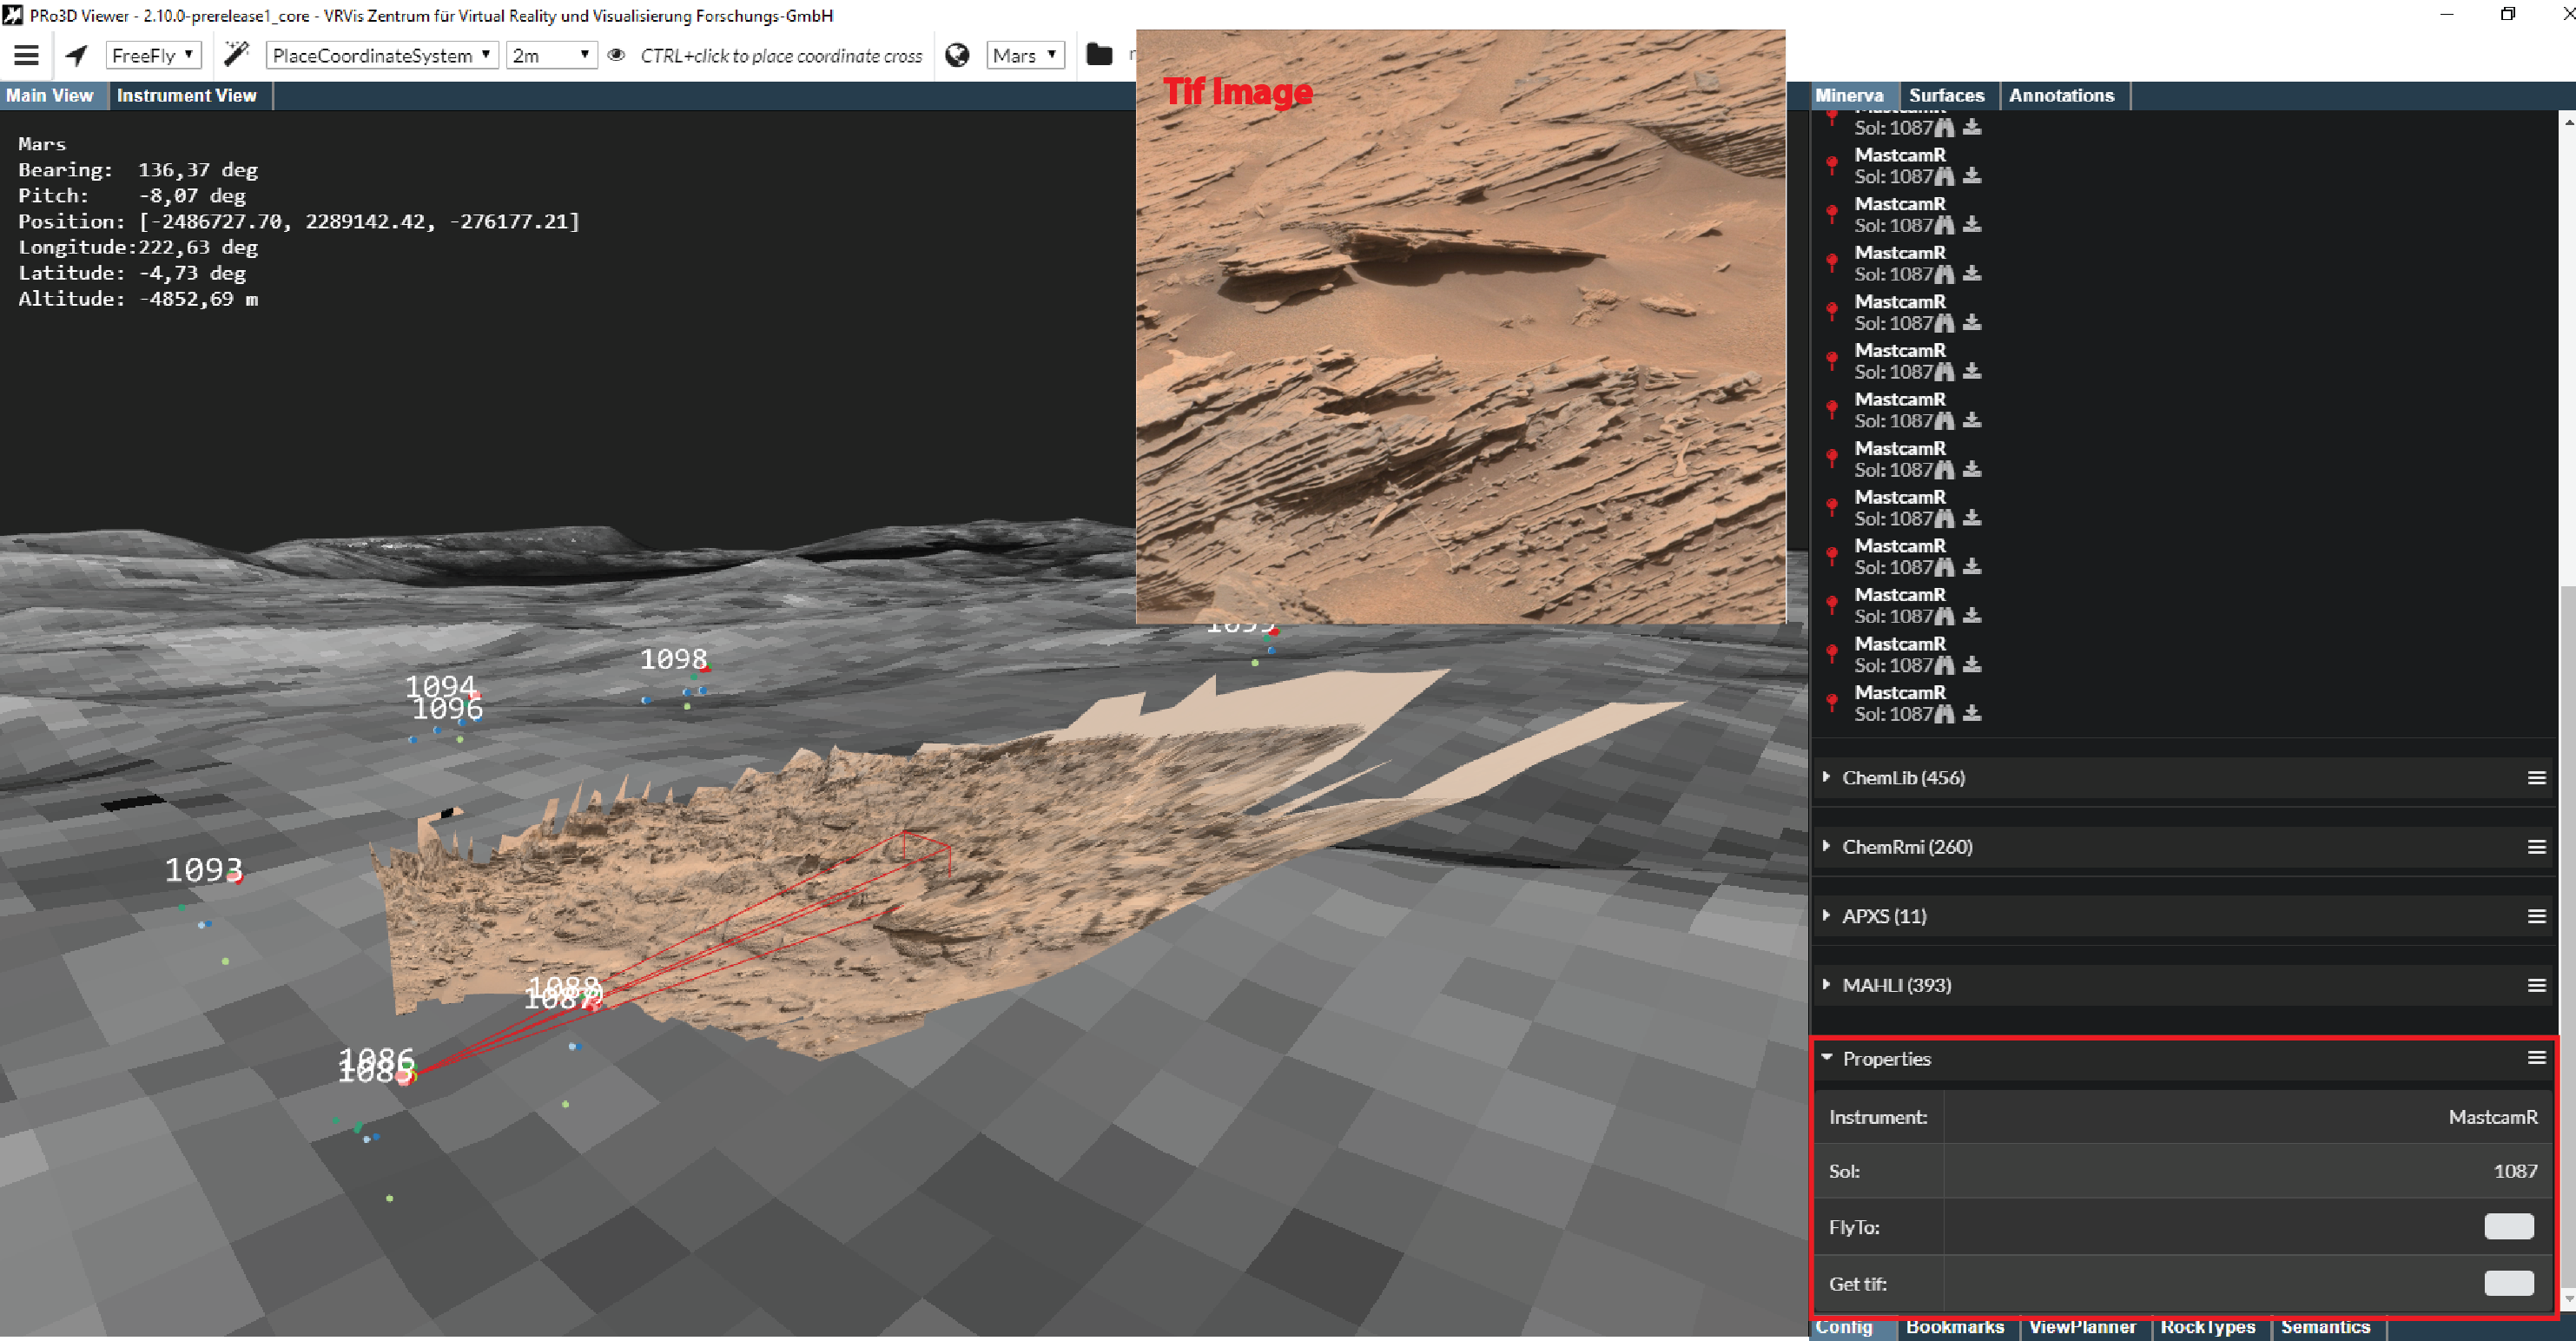
\includegraphics[width=1\textwidth]{pics/PropertiesAI.png}
				\caption[Product Properties]{The properties panel shows the sol number and provides interactions for the last selected product.}
				\label{fig:ProductProperties}
		 \end{figure}
		
The properties panel (Figure~\ref{fig:StartMinerva} D and Figure~\ref{fig:ProductProperties}) shows
\begin{itemize}
  \item \textbf{The Sol Number}
	\item \textbf{FlyTo}: A click on the button triggers a FlyTo animation.
	\item \textbf{GetTif}: Downloads the product's tif image. The image is stored in the \path{Release\netcoreapp2.0\MinervaData} folder.
\end{itemize}
of the last selected product.

%----------------------------------------------------------------------------------------
%	SubSection: Minerva Picking Actions
%----------------------------------------------------------------------------------------
\subsection{Picking Actions}
\label{sec:minervaPicking}

\begin{figure}[h]
				\centering
					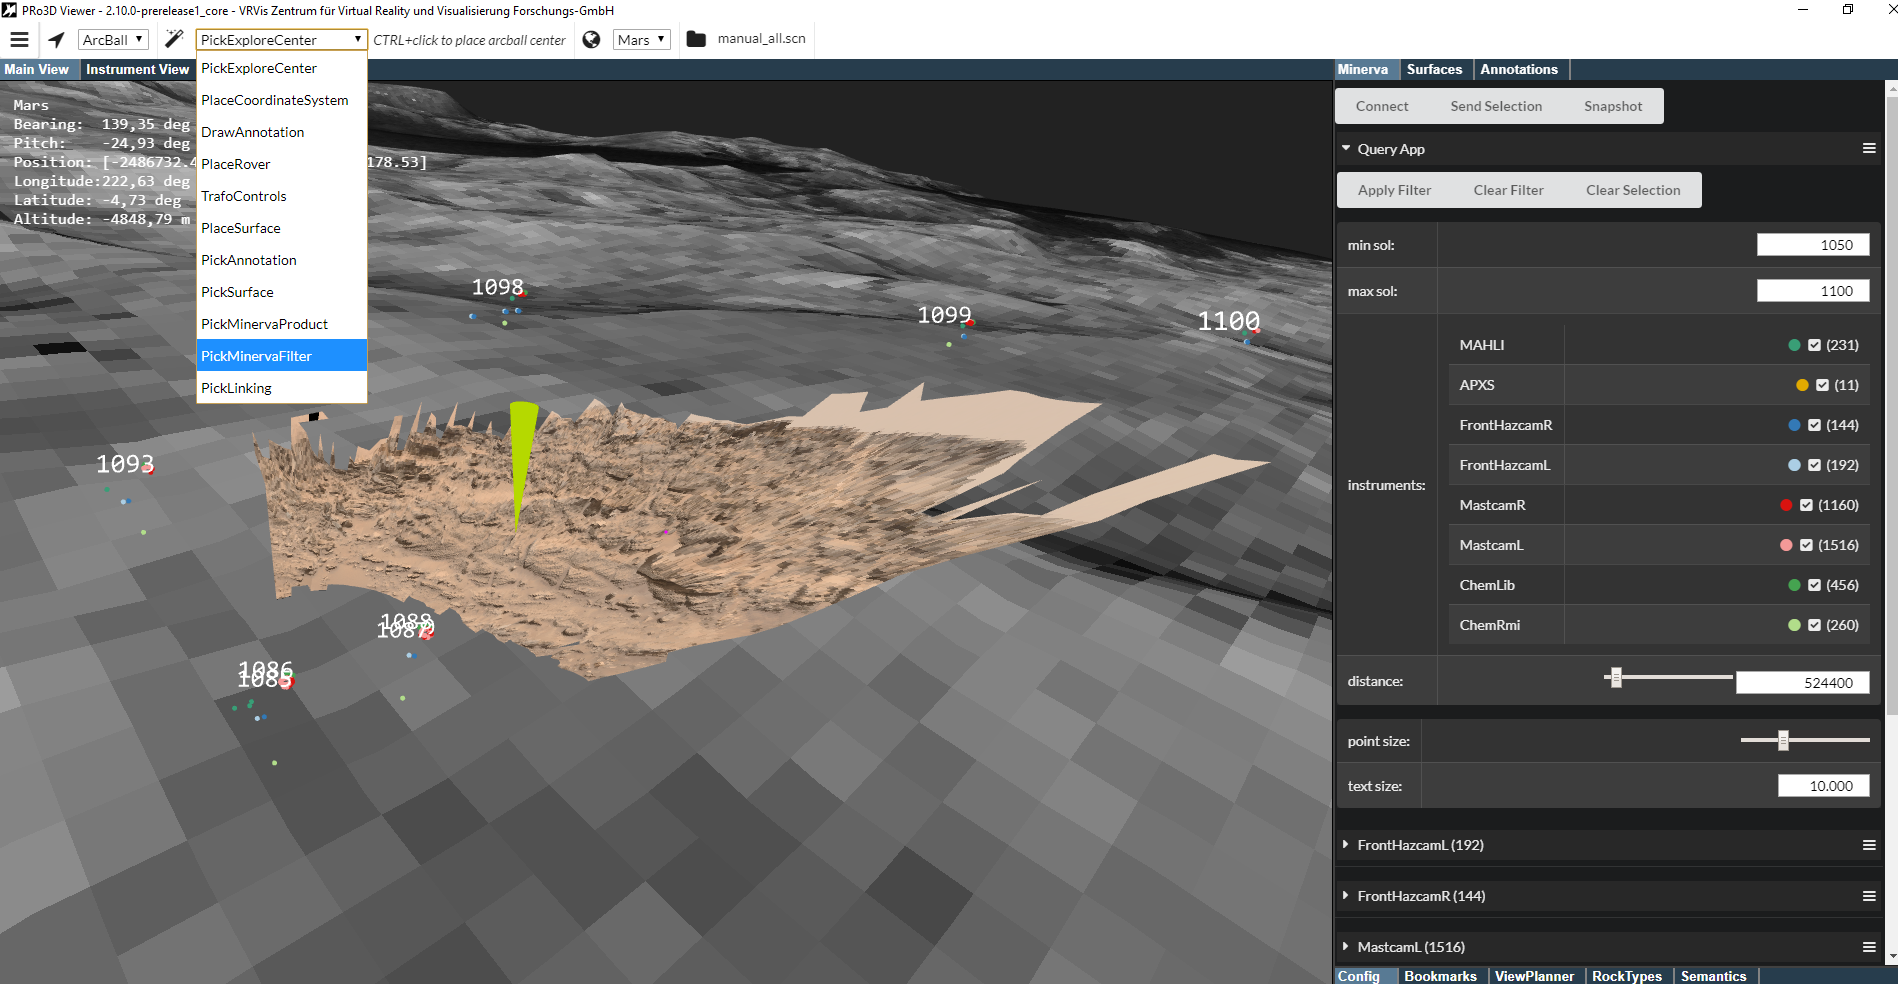
\includegraphics[width=1\textwidth]{pics/PickMinervaFilter.png}
				\caption[Pick Minerva Filter]{PickMinervaFilter}
				\label{fig:PickMinervaFilter}
		 \end{figure}
		
\begin{figure}[h]
				\centering
					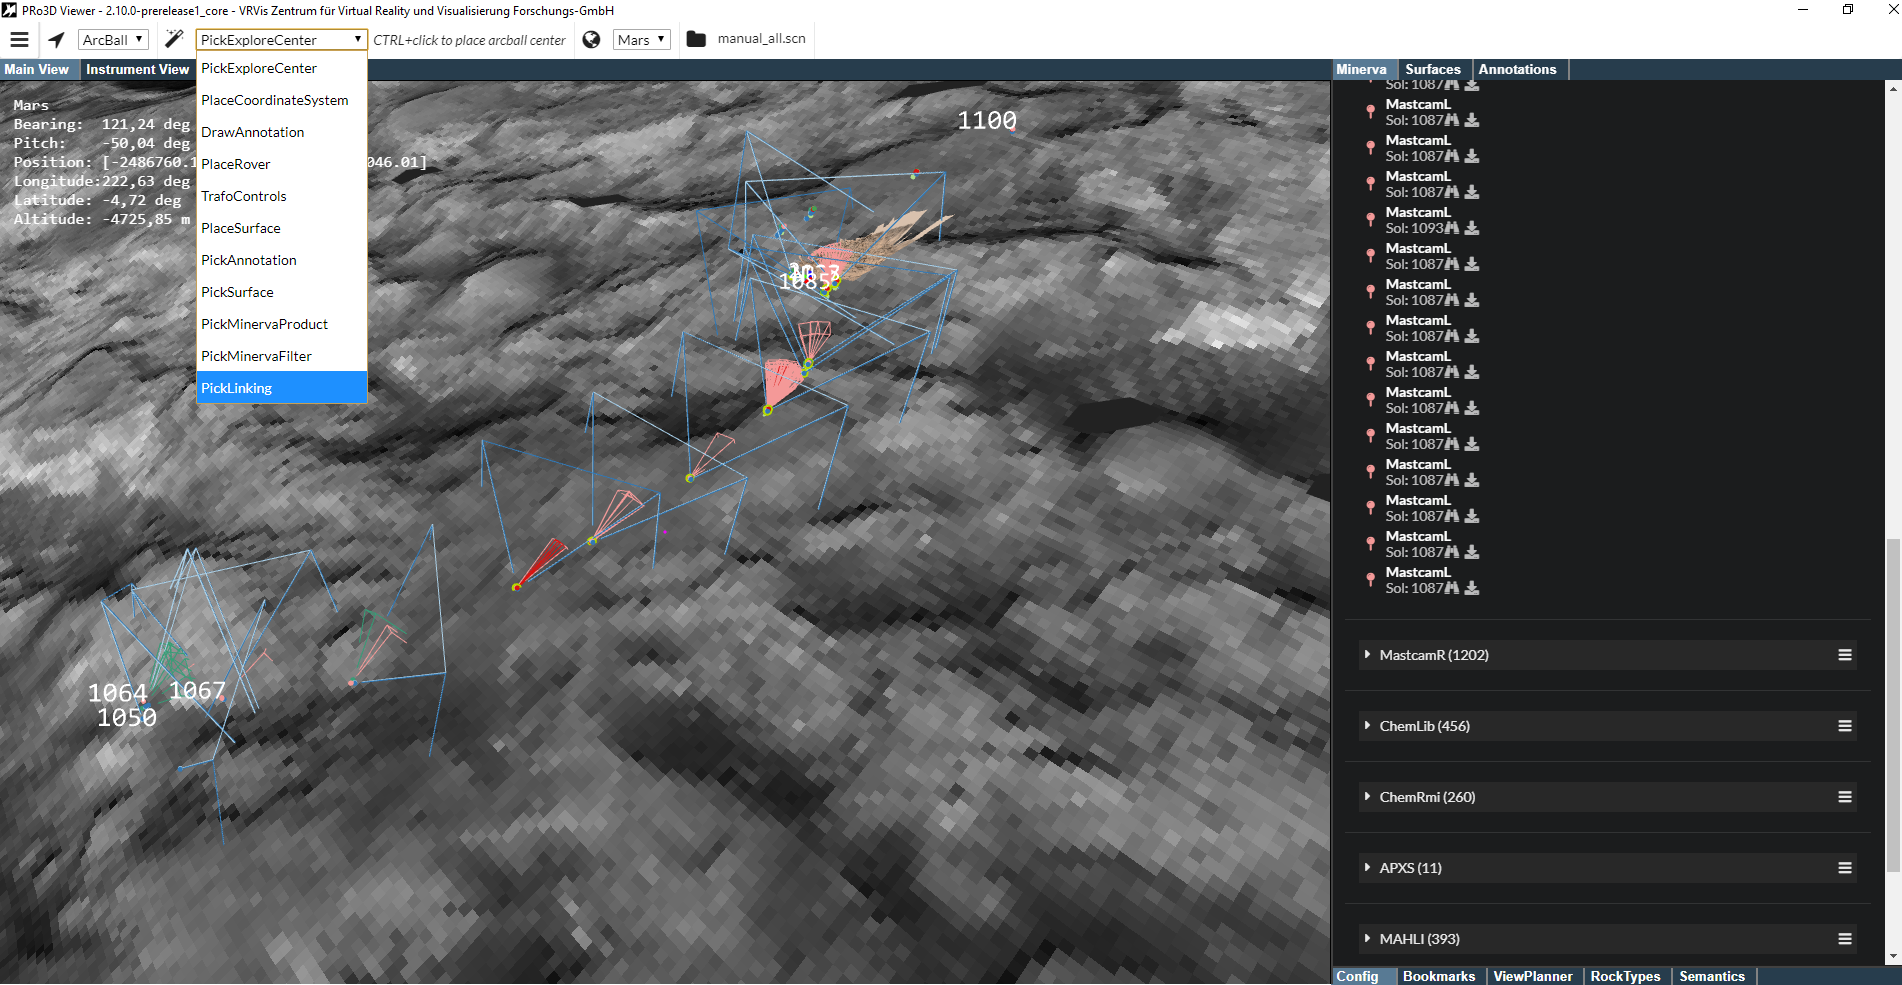
\includegraphics[width=1\textwidth]{pics/PickLinking1.png}
				\caption[Pick Linking]{PickLinking}
				\label{fig:PickLinking}
		 \end{figure}
		

There are three minerva picking actions in the picking actions drop down menu shown in Figure~\ref{fig:PickLinking}.
\\
\begin{itemize}
  \item \textbf{PickMinervaProduct}: You can set ``PickMinervaProduct'' in the actions menu to select a product in the Main View as described in Section~\ref{sec:selection}.
	\item \textbf{PickMinervaFilter}: Select ``PickMinervaFilter'' in the actions menu and press CTRL+LMB to pick a point on the surface. Then set a distance value with the distance slider in the Query App and click the ``ApplyFilter'' button. The products where the distance to the selected point is smaller than the selected distance in the Query App are shown (Figure~\ref{fig:PickMinervaFilter}).
	\item \textbf{PickLinking}: Select ``PickLinking'' in the actions menu and press CTRL+LMB to pick a point on the surface. All camera frustums of the products that captures the selected point are shown (Figure~\ref{fig:PickLinking}).
\end{itemize}


%----------------------------------------------------------------------------------------
%	Section: Command Line Interface
%----------------------------------------------------------------------------------------
%----------------------------------------------------------------------------------------
%	Section: PRo3D Command Line Interface
%----------------------------------------------------------------------------------------
\section{PRo3D Command Line Interface}

PRo3D can produce rendered images in a batch process via the command line. For this process, \emph{snapshot files} are used. They are in the JSON format, and contain transformations for each rendered image. There are two types of snapshot files: One type that only transforms camera parameters, and another that can be used to transform surfaces as well. This section describes the format of these files, and how they can be used with PRo3D to render an arbitrary number of images.

%----------------------------------------------------------------------------------------
%	SubSection: Start Command Line
%----------------------------------------------------------------------------------------
\subsection{PRo3D Snapshot Files}
\label{sec:snapshots}

Snapshot files have the JSON format, and need to follow a distinct scheme to be usable with PRo3D. Examples can be found in section \ref{cl:examples}.

Field of view and resolution of the resulting image are only specified once, at the beginning of the file. The parameter \textit{snapshots} contains one entry for each output image. Table  \ref{table:json} lists all available parameters of the format.

 \begin{center}
	\begin{table}
		\begin{tabular}{p{0.2\linewidth} p{0.12\linewidth} p{0.6\linewidth}}
		\textbf{Parameter}         & 		 & \textbf{Comment} \\
		\midrule
		fieldOfView 	  & required &\\ 
		resolution 		  & required & resolution of the output image\\  
		snapshots 		  & required & each entry in this list will result in one output image\\    
		filename 		  & required & name of the output file\\ 
		view 			  & required & camera parameters \\  
		forward           & required & forward vector of the camera\\
		location          & required & location of the camera\\
		up                & required & up vector of the camera\\
		surfaceUpdates    & optional & \\    		
		opcname 		  & required & name of the surface to be transformed\\    		
		trafo 			  & optional & transformation to be applied to the surface\\    		
		visible 		  & optional & visibility of the surface \\  			
		\specialrule{\lightrulewidth}{1.0pt}{4.0pt}				
	\end{tabular} 
	\label{table:json}
	\caption{Available parameters for a PRo3D Snapshot file}
	\end{table}
\end{center}



%----------------------------------------------------------------------------------------
%	SubSection: Minerva Features
%----------------------------------------------------------------------------------------
\subsection{Arguments and Features}
\label{sec:clArgs}

The \texttt{--help} flag will provide you with a full list of possible command line arguments for PRo3D. Table \ref{table:args} lists all available arguments.

\begin{lstlisting}
PRo3D.Viewer.exe --help
\end{lstlisting}

The simplest way to start the rendering process is to start PRo3D from the command line with only the path to the OPC file(s) and the snapshot file:

\begin{lstlisting}
PRo3D.Viewer.exe --opcs MyOPCs\firstOpc\;MyOPCs\secondOpc\ --asnap snapshots.JSON
\end{lstlisting}

The \texttt{--opcs} flag is followed by multiple paths to folders containing OPC surfaces separated with a semi colon. The \texttt{--asnap} flag is followed by the path to a snapshot file in the format described above, and as the examples in section \ref{cl:examples}. Make sure you are in the same directory as the \emph{PRo3D.Viewer.exe} file or specify the path to that file in the command. Paths can be either absolute or relative. The root of relative paths is the directory in which PRo3D.Viewer.exe is located. The flag \texttt{--snap} is used for legacy files which do not contain surface updates, and do not group the view parameters under a \emph{view} entry.\\

To specify an output folder use the \texttt{--out} flag:

\begin{lstlisting}
PRo3D.Viewer.exe --opcs MyOPCs\firstOpc\;MyOPCs\secondOpc\ --asnap snapshots.JSON --out MyImages\Renderd
\end{lstlisting}

If no output folder is specified, the images will be placed in the folder in which PRo3D.Viewer.exe is located. 

 \begin{center}
 	\begin{table}
		\begin{tabular}{p{0.3\linewidth} p{0.65\linewidth} }
			\textbf{Argument}          		 & \textbf{Description} \\
			\midrule
			--help                            &  show help\\
			--obj [path];[path];[path];[...]  &  load OBJ(s) from one or more paths\\
			--opc [path];[path];[path];[...]  &  load OPC(s) from one or more paths\\
			--asnap [path\textbackslash snapshot.json]      &  path to a snapshot file, refer to PRo3D User Manual for the correct format\\
			--out [path]                      &  path to a folder where output images will be saved; if the folder does not exist it will be created\\
			--renderDepth         &              render the depth map as well and save it as an additional image file\\
			--exitOnFinish                    &  quit PRo3D once all screenshots have been saved\\
			--verbose                         &  use verbose mode\\
			--excentre                        &  show exploration centre\\
			--refsystem                       &  show reference system\\
			--noMagFilter                     &  turn off linear texture magnification filtering\\
			--snap [path\textbackslash snapshot.json]       &  path to a snapshot file containing camera views (old format)\\
			\specialrule{\lightrulewidth}{1.0pt}{4.0pt}
		\end{tabular}    
	
	\caption{All arguments available for PRo3D's command line interface} 
	
	\label{table:args} 
	\end{table}
\end{center}

\subsection{Examples} \label{cl:examples}
 The examples listed below will result in two rendered images. By adding more blocks describing snapshots (beginning with curly brackets "filename", and ending with the corresponding closing curly bracket), any number of images can be produced. 

\lstinputlisting[language=json, caption={Snapshot file example with camera- and surface transformations.}, label=lst:json1]{snapshot.JSON}

\lstinputlisting[language=json, caption={Snapshot file example with camera transformations.}, label=lst:json2]{snapshot2.JSON}

\lstinputlisting[language=json, caption={Snapshot file example with surface transformations and visibility of the surfaces.}, label=lst:json3]{snapshot3.JSON}


%----------------------------------------------------------------------------------------
%	Section: Keyboard Shortcuts
%----------------------------------------------------------------------------------------
%----------------------------------------------------------------------------------------
%	Section: PRo3D Command Line Interface
%----------------------------------------------------------------------------------------
\section{PRo3D Keyboard Shortcuts}


\begin{center}
	\begin{table}[h!]
		\begin{tabular}{p{0.25\linewidth} p{0.7\linewidth} }
			\textbf{Shortcut}          		 & \textbf{Description} \\
			\midrule
			f           			&  toggle linear texture magnification filtering\\
			p						&  show/hide exploration point \\
			page up/down	    	&  raise/lower navigation sensitivity\\
			ctrl s					&  save existing scene (use the menu to save a new scene) \\
			ctrl c					&  print current camera parameters in snapshot format on the command line \\
			space					&  save waypoint \\
			F1  					&  Interaction: Pick Explore Center \\
			F2 					    &  Interaction: Draw Annotation \\
			F3 						&  Interaction: Pick Annotation \\
			F4						&  Interaction: Place Coordinate System \\
			\specialrule{\lightrulewidth}{1.0pt}{4.0pt}
		\end{tabular}    
		
		\caption{A List of keyboard shortcuts in PRo3D} 
		
		\label{table:args} 
	\end{table}
\end{center}

%----------------------------------------------------------------------------------------
%	END OF DOCUMENT
%----------------------------------------------------------------------------------------
\end{document}

